% ***************************************************
% A Classic Thesis Style
% An Homage to The Elements of Typographic Style
%
% Copyright (C) 2012 Andr\'e Miede http://www.miede.de
%
% If you like the style then I would appreciate a postcard. My
% address can be found in the file ClassicThesis.pdf. A collection
% of the postcards I received so far is available online at 
% http://postcards.miede.de
%
% License:
% This program is free software; you can redistribute it and/or
% modify it under the terms of the GNU General Public License as
% published by the Free Software Foundation; either version 2 of
% the License, or (at your option) any later version.
%
% This program is distributed in the hope that it will be useful,
% but WITHOUT ANY WARRANTY; without even the implied warranty of
% MERCHANTABILITY or FITNESS FOR A PARTICULAR PURPOSE.  See the
% GNU General Public License for more details.
%
% You should have received a copy of the GNU General Public
% License along with this program; see the file COPYING.  If not,
% write to the Free Software Foundation, Inc., 59 Temple Place -
% Suite 330, Boston, MA 02111-1307, USA.
%
% ***************************************************************
% Note:
%    * You must not use "u etc. in strings/commands that will be spaced out (use \"u or real umlauts instead)
%    * New enumeration (small caps): \begin{aenumerate} \end{aenumerate}
%    * For margin notes: \marginpar or \graffito{}
%    * Do not use bold fonts in this style, it is designed around them
%    * Use tables as in the examples
%    * See classicthesis-preamble.sty for useful commands
% ****************************************************************

\documentclass[ twoside, 
			openright,
			% letterpaper a4paper
			titlepage, 
			numbers=noenddot,
			headinclude, %1headlines
            		footinclude=true, 
			cleardoublepage=empty,
			abstractoff, % <--- obsolete, remove (todo)
			BCOR=5mm,
			paper=a4, 
			fontsize=11pt, %11pt,
			]{scrreprt}

%*****************************************************************
% Note: Make all your adjustments in here
%*****************************************************************
% \usepackage[backref, backend=biber]{biblatex}
\usepackage[backref,
		backend=bibtex,
            	maxbibnames=99,
            	natbib=true,
            	firstinits=false,
            	style=authoryear-comp,
            	sortcites=false,
            	doi=false,
            	url=false]{biblatex}
\bibliography{Bibliography}	

% ****************************************************************
% classicthesis-config.tex 
% formerly known as loadpackages.sty, classicthesis-ldpkg.sty, and
% classicthesis-preamble.sty Use it at the beginning of your
% ClassicThesis.tex, or as a LaTeX Preamble in your
% ClassicThesis.{tex,lyx} with % ****************************************************************
% classicthesis-config.tex 
% formerly known as loadpackages.sty, classicthesis-ldpkg.sty, and
% classicthesis-preamble.sty Use it at the beginning of your
% ClassicThesis.tex, or as a LaTeX Preamble in your
% ClassicThesis.{tex,lyx} with % ****************************************************************
% classicthesis-config.tex 
% formerly known as loadpackages.sty, classicthesis-ldpkg.sty, and
% classicthesis-preamble.sty Use it at the beginning of your
% ClassicThesis.tex, or as a LaTeX Preamble in your
% ClassicThesis.{tex,lyx} with \input{classicthesis-config}
% ****************************************************************
% If you like the classicthesis, then I would appreciate a
% postcard. My address can be found in the file
% ClassicThesis.pdf. A collection of the postcards I received so
% far is available online at http://postcards.miede.de
% ****************************************************************

% ****************************************************************
% 1. Configure classicthesis for your needs here, e.g., remove
% "drafting" below in order to deactivate the time-stamp on the
% pages
% ****************************************************************
\PassOptionsToPackage{eulerchapternumbers,
					listings,
					%drafting,
				 	pdfspacing,
					floatperchapter,
					%linedheaders,
				 	subfig,
					beramono,
					eulermath,
					parts}{classicthesis}										

% ****************************************************************
% Triggers for this config
% **************************************************************** 
\usepackage{ifthen}
\newboolean{enable-backrefs} % enable backrefs in the bibliography
\setboolean{enable-backrefs}{false} % true false
% TODO backref is incompatible?
% ****************************************************************
%*********************************************************************************
% 2.a Math
%*********************************************************************************
\PassOptionsToPackage{fleqn}{amsmath} % math environments and more by the AMS 
\usepackage{amsmath,amssymb}

\usepackage{amsthm}
\usepackage{amssymb}
\renewcommand\qedsymbol{$\blacksquare$}

\theoremstyle{definition}
\newtheorem{definition}{Definition}[chapter]
\newtheorem{theorem}{Theorem}[chapter]

\theoremstyle{plain}
\newtheorem{observation}[definition]{Observation}
\newtheorem{corollary}[theorem]{Corollary}
\newtheorem{lemma}[theorem]{Lemma}
\newtheorem{assumption}[theorem]{Assumption}
% **********************************************************************



% ****************************************************************
% 3. Personal data and user ad-hoc commands
% ****************************************************************
\newcommand{\myTitle}{Stochastic Variance Reduced Policy Gradient\xspace}
\newcommand{\myTitleIT}{Stochastic Variance Reduced Policy Gradient \xspace}
\newcommand{\myFirstAuthorName}{Damiano Binaghi\xspace}
\newcommand{\myMatrFirstAuthor}{858458\xspace}
\newcommand{\mySecondAuthorName}{Giuseppe Canonaco\xspace}
\newcommand{\myMatrSecondAuthor}{852749\xspace}
\newcommand{\mySupervisor}{Marcello Restelli\xspace} % relatore
\newcommand{\myOtherSupervisor}{Matteo Papini\xspace} % co relatori
\newcommand{\myOtherOtherSupervisor}{Matteo Pirotta\xspace}
\newcommand{\myCoExaminer}{\xspace} % contro-relatore
\newcommand{\myFaculty}{Facolt\`a di Ingegneria\xspace}
\newcommand{\mySchool}{Scuola di Ingegneria Industriale e dell\textquotesingle Informazione\xspace}
\newcommand{\myDepartment}{Dipartimento di Elettronica, Informazione e Bioingegneria\xspace}
\newcommand{\myCourseFirstPart}{Master of Science in\xspace}
\newcommand{\myCourseFirstPartIT}{Corso di Laurea Magistrale in\xspace}
\newcommand{\myCourseSecondPart}{Computer Science and Engineering\xspace}
\newcommand{\myCourseSecondPartIT}{Ingegneria Informatica\xspace}
\newcommand{\myUni}{Politecnico di Milano\xspace}
\newcommand{\myLocation}{Milan\xspace}
\newcommand{\myTime}{April 2018\xspace}
\newcommand{\myVersion}{version 1.0\xspace}
\newcommand{\myAcademicYear}{Academic Year 2017-2018\xspace}
\newcommand{\myAcademicYearIT}{Anno Accademico 2017-2018\xspace}




% ********************************************************************
% Setup, fine tuning, and useful commands
% ********************************************************************
\newcounter{dummy} % necessary for correct hyperlinks (to index, bib, etc.)
\newlength{\abcd} % for ab..z string length calculation
\providecommand{\mLyX}{L\kern-.1667em\lower.25em\hbox{Y}\kern-.125emX\@}
% from here till the end of the section, you can modify whatever you want
\newcommand{\ie}{i.\,e.\ }
\newcommand{\Ie}{I.\,e.\ }
\newcommand{\eg}{e.\,g.\ }
\newcommand{\Eg}{E.\,g.\ }
% referencing commands
\newcommand{\myEq}[1]{equation \eqref{#1}}
\newcommand{\MyEq}[1]{Equation \eqref{#1}}
\newcommand{\myFig}[1]{figure \ref{#1}}
\newcommand{\MyFig}[1]{Figure \ref{#1}}
\newcommand{\myTab}[1]{table \ref{#1}}
\newcommand{\MyTab}[1]{Table \ref{#1}}
\newcommand{\mySubsec}[1]{subsection \ref{#1}}
\newcommand{\MySubsec}[1]{Subsection \ref{#1}}
\newcommand{\mySec}[1]{section \ref{#1}}
\newcommand{\MySec}[1]{Section \ref{#1}}
\newcommand{\myChap}[1]{chapter \ref{#1}}
\newcommand{\MyChap}[1]{Chapter \ref{#1}}
\newcommand{\myAppendix}[1]{appendix \ref{#1}}
\newcommand{\MyAppendix}[1]{Appendix \ref{#1}}
\newcommand{\myEmph}[1]{\textsc{#1}}

% **********************************************************************
%%%CUSTOM COMMANDS%%%
%***********************************************************************
%Math
\newcommand{\realspace}{\mathbb R}      % realspace
\newcommand{\transpose}[1]{{#1}^\texttt{T}}
\DeclareMathOperator*{\argmax}{arg\,max}
\DeclareMathOperator*{\argmin}{arg\,min}
\DeclareMathOperator*{\EV}{\mathbb{E}}
\DeclareMathOperator{\Tr}{Tr}
\DeclareMathOperator*{\Cov}{\mathbb{C}ov}
\DeclareMathOperator*{\Var}{\mathbb{V}ar}
\newcommand{\EVV}[2][\ppvect \in \ppspace]{\EV_{#1}\left[{#2}\right]}
\newcommand{\norm}[2][\infty]{\left\|#2\right\|_{#1}}
\newcommand{\Dij}[2]{\frac{\partial^{2}{#1}}{\partial{#2}_i\partial{#2}_j}}
\newcommand{\de}{\,\mathrm{d}}
\newcommand{\dotprod}[2]{\left\langle#1,#2\right\rangle}
\newcommand{\dnabla}{\nabla\!\!\!\!\nabla}
%RL
\newcommand{\vtheta}{\boldsymbol{\theta}}
\newcommand{\Aspace}{\mathcal{A}}
\newcommand{\Sspace}{\mathcal{S}}
\newcommand{\Tspace}{\mathcal{T}}
\newcommand{\Transition}{\mathcal{P}}
\newcommand{\Reward}{\mathcal{R}}
\newcommand{\stationary}{d_{\rho}^{\pi_{\vtheta}}(s)}
\newcommand{\policy}{\pi_{\vtheta}(a \vert s)}
\newcommand{\pol}{\pi_{\vtheta}}
\newcommand{\trajdistr}{\pi_{\vtheta}(\tau)}
\newcommand{\score}[2]{\nabla\log p_{#1}(#2)}
\newcommand{\Qfun}{Q^{\pi_{\vtheta}}(s,a)}
\newcommand{\Vfun}{V^{\pi_{\vtheta}}(s)}
\newcommand{\vTheta}{\boldsymbol{\Theta}}
\newcommand{\vphi}{\boldsymbol{\phi}}
\newcommand{\gradJ}[1]{\nabla J(#1)}
\newcommand{\gradApp}[2]{\widehat{\nabla}_{#2}J(#1)}
\newcommand{\eqdef}{\mathrel{\mathop:}=}
\newcommand{\Dataset}{\mathcal{D}}
%Specific
\newcommand{\Ets}[2][t]{\mathbb{E}_{#1\vert s}\left[#2\right]}
\newcommand{\Es}[1]{\mathbb{E}_{s}\left[#1\right]}
\newcommand{\Covts}[3][t]{{\mathbb{C}\text{ov}}_{#1\vert s}\left(#2,#3\right)}
\newcommand{\Covs}[2]{{\mathbb{C}\text{ov}}_{s}\left(#1,#2\right)}
\newcommand{\Varts}[2][t]{{\mathbb{V}\text{ar}}_{#1\vert s}\left[#2\right]}
\newcommand{\Vars}[1]{{\mathbb{V}\text{ar}}_{s}\left[#1\right]}
\newcommand{\gradBlack}[1]{\blacktriangledown J(#1)}
\newcommand{\gradIdeal}[1]{\dnabla J(#1)}
\newcommand{\VARRF}{V}
\newcommand{\GRADLOG}{G}
\newcommand{\VARIS}{W}
\newcommand{\HESSLOG}{F}
% short forms 
\newcommand{\wt}[1]{\widetilde{#1}}
\newcommand{\wh}[1]{\widehat{#1}}
\newcommand{\wo}[1]{\overline{#1}}
\newcommand{\wb}[1]{\overline{#1}}
%%%%%%


% **********************************************************************
% 3. Loading some handy packages
% **********************************************************************
\PassOptionsToPackage{fleqn}{amsmath} % math environments and more by the AMS 
\usepackage{amsmath}
\usepackage{algorithm}
\usepackage{algorithmic}
\usepackage{amsthm}
\usepackage{amssymb}
\usepackage{geometry}
\renewcommand\qedsymbol{$\blacksquare$}		

\PassOptionsToPackage{autostyle,italian=guillemets,threshold=2}{csquotes}
 	\usepackage{csquotes}

\PassOptionsToPackage{american,italian}{babel}
	 \usepackage{babel}

 \usepackage{textcomp} % fix warning with missing font shapes
\usepackage{scrhack} % fix warnings when using KOMA with listings package          
\usepackage{xspace} % to get the spacing after macros right  
\usepackage{mparhack} % get marginpar right
\usepackage{fixltx2e} % fixes some LaTeX stuff
\usepackage{microtype}
\usepackage[normalem]{ulem} % to have strikethrough text

\PassOptionsToPackage{printonlyused,smaller}{acronym}
	\usepackage{acronym} % nice macros for handling all acronyms in the thesis
% **********************************************************************
% Recommended, but optional, packages for figures and better typesetting:
\usepackage{microtype}
\usepackage{graphicx}
\graphicspath{ {images/} }


\usepackage{microtype}
\usepackage{graphicx}
\graphicspath{ {images/} }
%\usepackage{subfigure}
\usepackage{booktabs} % for professional tables

% hyperref makes hyperlinks in the resulting PDF.
% If your build breaks (sometimes temporarily if a hyperlink spans a page)
% please comment out the following usepackage line and replace
% \usepackage{icml2018} with \usepackage[nohyperref]{icml2018} above.
\usepackage{hyperref}
%%%USEFUL PACKAGES%%%
\usepackage{nicefrac}       % compact symbols for 1/2, etc.
\usepackage{mathtools}
\usepackage{pifont}
\usepackage[makeroom]{cancel}
\usepackage{placeins}

%e.g. ...
\usepackage{xspace}
\DeclareRobustCommand{\eg}{e.g.,\@\xspace}
\DeclareRobustCommand{\ie}{i.e.,\@\xspace}
\DeclareRobustCommand{\wrt}{w.r.t.\@\xspace}



% **********************************************************************
% 4. Setup floats: tables, (sub)figures, and captions
% **********************************************************************
\usepackage{tabularx} % better tables
	\setlength{\extrarowheight}{3pt} % increase table row height
\newcommand{\tableheadline}[2]{\multicolumn{1}{#1}{\normalsize\spacedlowsmallcaps{#2}}}
\newcommand{\tableheadlineMore}[3]{\multicolumn{#1}{#2}{\normalsize\spacedlowsmallcaps{#3}}}
\newcommand{\tablefirstcol}[2]{\multicolumn{1}{#1}{\textbf{#2}}}

\usepackage{caption}
	\captionsetup{format=hang,labelfont={sf,bf},font=small}
\usepackage{colortbl}
\usepackage{multirow}

\usepackage{subfig}
\usepackage{siunitx}
% *********************************************************************


% *********************************************************************
% 5. Setup code listings
% *********************************************************************
\usepackage{listings}
\lstloadlanguages{bash, C++, Java, Matlab}

% for special keywords
\lstset{language=[LaTeX]Tex,
    keywordstyle=\color{RoyalBlue},%\bfseries,
    basicstyle=\small\ttfamily,
    %identifierstyle=\color{NavyBlue},
    commentstyle=\color{Green}\ttfamily,
    stringstyle=\rmfamily,
    numbers=none,%left,%
    numberstyle=\scriptsize,%\tiny
    stepnumber=5,
    numbersep=8pt,
    showstringspaces=false,
    breaklines=true,
    frameround=ftff,
    frame=single,
    belowcaptionskip=.75\baselineskip
    %frame=L
} 
% *********************************************************************


% *********************************************************************
% 6. PDFLaTeX, hyperreferences and citation backreferences
% *********************************************************************
% ********************************************************************
% Using PDFLaTeX
% ********************************************************************
\PassOptionsToPackage{pdftex,hyperfootnotes=false,pdfpagelabels}{hyperref}
	\usepackage{hyperref}  % backref linktocpage pagebackref
\pdfcompresslevel=9
\pdfadjustspacing=1 
\PassOptionsToPackage{pdftex}{graphicx}
	\usepackage{graphicx} 

% ********************************************************************
% Setup the style of the backrefs from the bibliography
% (translate the options to any language you use)
% ********************************************************************
\newcommand{\backrefnotcitedstring}{\relax}%(Not cited.)
\newcommand{\backrefcitedsinglestring}[1]{(Cited on page~#1.)}
\newcommand{\backrefcitedmultistring}[1]{(Cited on pages~#1.)}
\ifthenelse{\boolean{enable-backrefs}}%
{%
		\PassOptionsToPackage{hyperpageref}{backref}
		\usepackage{backref} % to be loaded after hyperref package 
		   \renewcommand{\backreftwosep}{ and~} % separate 2 pages
		   \renewcommand{\backreflastsep}{, and~} % separate last of longer list
		   \renewcommand*{\backref}[1]{}  % disable standard
		   \renewcommand*{\backrefalt}[4]{% detailed backref
		      \ifcase #1 %
		         \backrefnotcitedstring%
		      \or%
		         \backrefcitedsinglestring{#2}%
		      \else%
		         \backrefcitedmultistring{#2}%
		      \fi}%
}{\relax}    


% ****************************************************************
% PDF/A compliance
% ****************************************************************
% TODO not working: requires downloading color specification file in a specific
% tex folder and other hacks I don't want to spend time with
% \usepackage[a-1b]{pdfx}

% ********************************************************************
% Hyperreferences
% ********************************************************************
\hypersetup{%
    %draft,	% = no hyperlinking at all (useful in b/w printouts)
    colorlinks=true, linktocpage=true, pdfstartpage=3, pdfstartview=FitV,%
    % uncomment the following line if you want to have black links (e.g., for printing)
    %colorlinks=false, linktocpage=false, pdfborder={0 0 0}, pdfstartpage=3, pdfstartview=FitV,% 
    breaklinks=true, pdfpagemode=UseNone, pageanchor=true, pdfpagemode=UseOutlines,%
    plainpages=false, bookmarksnumbered, bookmarksopen=true, bookmarksopenlevel=1,%
    hypertexnames=true, pdfhighlight=/O,%nesting=true,%frenchlinks,%
    urlcolor=webbrown, linkcolor=RoyalBlue, citecolor=webgreen, %pagecolor=RoyalBlue,%
    %urlcolor=Black, linkcolor=Black, citecolor=Black, %pagecolor=Black,%
} 

    %pdftitle={\myTitle},%
    %pdfauthor={\textcopyright\ \myFirstAuthorName and \mySecondAuthorName, \myUni, \myFaculty},%
    %pdfsubject={},%
    %pdfkeywords={},%
    %pdfcreator={pdfLaTeX},%
    %pdfproducer={LaTeX with hyperref and classicthesis}%

%}   

% ********************************************************************
% Setup autoreferences
% ********************************************************************
% There are some issues regarding autorefnames
% http://www.ureader.de/msg/136221647.aspx
% http://www.tex.ac.uk/cgi-bin/texfaq2html?label=latexwords
% you have to redefine the makros for the 
% language you use, e.g., american, ngerman
% (as chosen when loading babel/AtBeginDocument)
% ********************************************************************
\makeatletter
\@ifpackageloaded{babel}%
    {%
       \addto\extrasamerican{%
					\renewcommand*{\figureautorefname}{Figure}%
					\renewcommand*{\tableautorefname}{Table}%
					\renewcommand*{\partautorefname}{Part}%
					\renewcommand*{\chapterautorefname}{Chapter}%
					\renewcommand*{\sectionautorefname}{Section}%
					\renewcommand*{\subsectionautorefname}{Section}%
					\renewcommand*{\subsubsectionautorefname}{Section}% 	
				}%
       \addto\extrasitalian{% 
					\renewcommand*{\paragraphautorefname}{Paragrafo}%
					\renewcommand*{\subparagraphautorefname}{Paragrafo}%
					\renewcommand*{\footnoteautorefname}{Nota a pié di pagina}%
					\renewcommand*{\FancyVerbLineautorefname}{Zeile}%
					\renewcommand*{\theoremautorefname}{Teorema}%
					\renewcommand*{\appendixautorefname}{Appendice}%
					\renewcommand*{\equationautorefname}{Equazione}%        
					\renewcommand*{\itemautorefname}{Punto}%
				}%	
			% Fix to getting autorefs for subfigures right (thanks to Belinda Vogt for changing the definition)
			\providecommand{\subfigureautorefname}{\figureautorefname}%  			
    }{\relax}
\makeatother

% ****************************************************************
% 7. Last calls before the bar closes
% ****************************************************************

\usepackage{classicthesis} 

% ****************************************************************

\makeatletter
\newenvironment{myalign*}{\ifvmode\else\hfil\null\linebreak\fi
	\hspace*{-\leftmargin}\minipage\textwidth
	%\setlength{\abovedisplayskip}{0pt}%
	\setlength{\abovedisplayshortskip}{\abovedisplayskip}%
	\start@align\@ne\st@rredtrue\m@ne}%
{\endalign\endminipage\linebreak\linebreak}
\makeatother
% ****************************************************************
% If you like the classicthesis, then I would appreciate a
% postcard. My address can be found in the file
% ClassicThesis.pdf. A collection of the postcards I received so
% far is available online at http://postcards.miede.de
% ****************************************************************

% ****************************************************************
% 1. Configure classicthesis for your needs here, e.g., remove
% "drafting" below in order to deactivate the time-stamp on the
% pages
% ****************************************************************
\PassOptionsToPackage{eulerchapternumbers,
					listings,
					%drafting,
				 	pdfspacing,
					floatperchapter,
					%linedheaders,
				 	subfig,
					beramono,
					eulermath,
					parts}{classicthesis}										

% ****************************************************************
% Triggers for this config
% **************************************************************** 
\usepackage{ifthen}
\newboolean{enable-backrefs} % enable backrefs in the bibliography
\setboolean{enable-backrefs}{false} % true false
% TODO backref is incompatible?
% ****************************************************************
%*********************************************************************************
% 2.a Math
%*********************************************************************************
\PassOptionsToPackage{fleqn}{amsmath} % math environments and more by the AMS 
\usepackage{amsmath,amssymb}

\usepackage{amsthm}
\usepackage{amssymb}
\renewcommand\qedsymbol{$\blacksquare$}

\theoremstyle{definition}
\newtheorem{definition}{Definition}[chapter]
\newtheorem{theorem}{Theorem}[chapter]

\theoremstyle{plain}
\newtheorem{observation}[definition]{Observation}
\newtheorem{corollary}[theorem]{Corollary}
\newtheorem{lemma}[theorem]{Lemma}
\newtheorem{assumption}[theorem]{Assumption}
% **********************************************************************



% ****************************************************************
% 3. Personal data and user ad-hoc commands
% ****************************************************************
\newcommand{\myTitle}{Stochastic Variance Reduced Policy Gradient\xspace}
\newcommand{\myTitleIT}{Stochastic Variance Reduced Policy Gradient \xspace}
\newcommand{\myFirstAuthorName}{Damiano Binaghi\xspace}
\newcommand{\myMatrFirstAuthor}{858458\xspace}
\newcommand{\mySecondAuthorName}{Giuseppe Canonaco\xspace}
\newcommand{\myMatrSecondAuthor}{852749\xspace}
\newcommand{\mySupervisor}{Marcello Restelli\xspace} % relatore
\newcommand{\myOtherSupervisor}{Matteo Papini\xspace} % co relatori
\newcommand{\myOtherOtherSupervisor}{Matteo Pirotta\xspace}
\newcommand{\myCoExaminer}{\xspace} % contro-relatore
\newcommand{\myFaculty}{Facolt\`a di Ingegneria\xspace}
\newcommand{\mySchool}{Scuola di Ingegneria Industriale e dell\textquotesingle Informazione\xspace}
\newcommand{\myDepartment}{Dipartimento di Elettronica, Informazione e Bioingegneria\xspace}
\newcommand{\myCourseFirstPart}{Master of Science in\xspace}
\newcommand{\myCourseFirstPartIT}{Corso di Laurea Magistrale in\xspace}
\newcommand{\myCourseSecondPart}{Computer Science and Engineering\xspace}
\newcommand{\myCourseSecondPartIT}{Ingegneria Informatica\xspace}
\newcommand{\myUni}{Politecnico di Milano\xspace}
\newcommand{\myLocation}{Milan\xspace}
\newcommand{\myTime}{April 2018\xspace}
\newcommand{\myVersion}{version 1.0\xspace}
\newcommand{\myAcademicYear}{Academic Year 2017-2018\xspace}
\newcommand{\myAcademicYearIT}{Anno Accademico 2017-2018\xspace}




% ********************************************************************
% Setup, fine tuning, and useful commands
% ********************************************************************
\newcounter{dummy} % necessary for correct hyperlinks (to index, bib, etc.)
\newlength{\abcd} % for ab..z string length calculation
\providecommand{\mLyX}{L\kern-.1667em\lower.25em\hbox{Y}\kern-.125emX\@}
% from here till the end of the section, you can modify whatever you want
\newcommand{\ie}{i.\,e.\ }
\newcommand{\Ie}{I.\,e.\ }
\newcommand{\eg}{e.\,g.\ }
\newcommand{\Eg}{E.\,g.\ }
% referencing commands
\newcommand{\myEq}[1]{equation \eqref{#1}}
\newcommand{\MyEq}[1]{Equation \eqref{#1}}
\newcommand{\myFig}[1]{figure \ref{#1}}
\newcommand{\MyFig}[1]{Figure \ref{#1}}
\newcommand{\myTab}[1]{table \ref{#1}}
\newcommand{\MyTab}[1]{Table \ref{#1}}
\newcommand{\mySubsec}[1]{subsection \ref{#1}}
\newcommand{\MySubsec}[1]{Subsection \ref{#1}}
\newcommand{\mySec}[1]{section \ref{#1}}
\newcommand{\MySec}[1]{Section \ref{#1}}
\newcommand{\myChap}[1]{chapter \ref{#1}}
\newcommand{\MyChap}[1]{Chapter \ref{#1}}
\newcommand{\myAppendix}[1]{appendix \ref{#1}}
\newcommand{\MyAppendix}[1]{Appendix \ref{#1}}
\newcommand{\myEmph}[1]{\textsc{#1}}

% **********************************************************************
%%%CUSTOM COMMANDS%%%
%***********************************************************************
%Math
\newcommand{\realspace}{\mathbb R}      % realspace
\newcommand{\transpose}[1]{{#1}^\texttt{T}}
\DeclareMathOperator*{\argmax}{arg\,max}
\DeclareMathOperator*{\argmin}{arg\,min}
\DeclareMathOperator*{\EV}{\mathbb{E}}
\DeclareMathOperator{\Tr}{Tr}
\DeclareMathOperator*{\Cov}{\mathbb{C}ov}
\DeclareMathOperator*{\Var}{\mathbb{V}ar}
\newcommand{\EVV}[2][\ppvect \in \ppspace]{\EV_{#1}\left[{#2}\right]}
\newcommand{\norm}[2][\infty]{\left\|#2\right\|_{#1}}
\newcommand{\Dij}[2]{\frac{\partial^{2}{#1}}{\partial{#2}_i\partial{#2}_j}}
\newcommand{\de}{\,\mathrm{d}}
\newcommand{\dotprod}[2]{\left\langle#1,#2\right\rangle}
\newcommand{\dnabla}{\nabla\!\!\!\!\nabla}
%RL
\newcommand{\vtheta}{\boldsymbol{\theta}}
\newcommand{\Aspace}{\mathcal{A}}
\newcommand{\Sspace}{\mathcal{S}}
\newcommand{\Tspace}{\mathcal{T}}
\newcommand{\Transition}{\mathcal{P}}
\newcommand{\Reward}{\mathcal{R}}
\newcommand{\stationary}{d_{\rho}^{\pi_{\vtheta}}(s)}
\newcommand{\policy}{\pi_{\vtheta}(a \vert s)}
\newcommand{\pol}{\pi_{\vtheta}}
\newcommand{\trajdistr}{\pi_{\vtheta}(\tau)}
\newcommand{\score}[2]{\nabla\log p_{#1}(#2)}
\newcommand{\Qfun}{Q^{\pi_{\vtheta}}(s,a)}
\newcommand{\Vfun}{V^{\pi_{\vtheta}}(s)}
\newcommand{\vTheta}{\boldsymbol{\Theta}}
\newcommand{\vphi}{\boldsymbol{\phi}}
\newcommand{\gradJ}[1]{\nabla J(#1)}
\newcommand{\gradApp}[2]{\widehat{\nabla}_{#2}J(#1)}
\newcommand{\eqdef}{\mathrel{\mathop:}=}
\newcommand{\Dataset}{\mathcal{D}}
%Specific
\newcommand{\Ets}[2][t]{\mathbb{E}_{#1\vert s}\left[#2\right]}
\newcommand{\Es}[1]{\mathbb{E}_{s}\left[#1\right]}
\newcommand{\Covts}[3][t]{{\mathbb{C}\text{ov}}_{#1\vert s}\left(#2,#3\right)}
\newcommand{\Covs}[2]{{\mathbb{C}\text{ov}}_{s}\left(#1,#2\right)}
\newcommand{\Varts}[2][t]{{\mathbb{V}\text{ar}}_{#1\vert s}\left[#2\right]}
\newcommand{\Vars}[1]{{\mathbb{V}\text{ar}}_{s}\left[#1\right]}
\newcommand{\gradBlack}[1]{\blacktriangledown J(#1)}
\newcommand{\gradIdeal}[1]{\dnabla J(#1)}
\newcommand{\VARRF}{V}
\newcommand{\GRADLOG}{G}
\newcommand{\VARIS}{W}
\newcommand{\HESSLOG}{F}
% short forms 
\newcommand{\wt}[1]{\widetilde{#1}}
\newcommand{\wh}[1]{\widehat{#1}}
\newcommand{\wo}[1]{\overline{#1}}
\newcommand{\wb}[1]{\overline{#1}}
%%%%%%


% **********************************************************************
% 3. Loading some handy packages
% **********************************************************************
\PassOptionsToPackage{fleqn}{amsmath} % math environments and more by the AMS 
\usepackage{amsmath}
\usepackage{algorithm}
\usepackage{algorithmic}
\usepackage{amsthm}
\usepackage{amssymb}
\usepackage{geometry}
\renewcommand\qedsymbol{$\blacksquare$}		

\PassOptionsToPackage{autostyle,italian=guillemets,threshold=2}{csquotes}
 	\usepackage{csquotes}

\PassOptionsToPackage{american,italian}{babel}
	 \usepackage{babel}

 \usepackage{textcomp} % fix warning with missing font shapes
\usepackage{scrhack} % fix warnings when using KOMA with listings package          
\usepackage{xspace} % to get the spacing after macros right  
\usepackage{mparhack} % get marginpar right
\usepackage{fixltx2e} % fixes some LaTeX stuff
\usepackage{microtype}
\usepackage[normalem]{ulem} % to have strikethrough text

\PassOptionsToPackage{printonlyused,smaller}{acronym}
	\usepackage{acronym} % nice macros for handling all acronyms in the thesis
% **********************************************************************
% Recommended, but optional, packages for figures and better typesetting:
\usepackage{microtype}
\usepackage{graphicx}
\graphicspath{ {images/} }


\usepackage{microtype}
\usepackage{graphicx}
\graphicspath{ {images/} }
%\usepackage{subfigure}
\usepackage{booktabs} % for professional tables

% hyperref makes hyperlinks in the resulting PDF.
% If your build breaks (sometimes temporarily if a hyperlink spans a page)
% please comment out the following usepackage line and replace
% \usepackage{icml2018} with \usepackage[nohyperref]{icml2018} above.
\usepackage{hyperref}
%%%USEFUL PACKAGES%%%
\usepackage{nicefrac}       % compact symbols for 1/2, etc.
\usepackage{mathtools}
\usepackage{pifont}
\usepackage[makeroom]{cancel}
\usepackage{placeins}

%e.g. ...
\usepackage{xspace}
\DeclareRobustCommand{\eg}{e.g.,\@\xspace}
\DeclareRobustCommand{\ie}{i.e.,\@\xspace}
\DeclareRobustCommand{\wrt}{w.r.t.\@\xspace}



% **********************************************************************
% 4. Setup floats: tables, (sub)figures, and captions
% **********************************************************************
\usepackage{tabularx} % better tables
	\setlength{\extrarowheight}{3pt} % increase table row height
\newcommand{\tableheadline}[2]{\multicolumn{1}{#1}{\normalsize\spacedlowsmallcaps{#2}}}
\newcommand{\tableheadlineMore}[3]{\multicolumn{#1}{#2}{\normalsize\spacedlowsmallcaps{#3}}}
\newcommand{\tablefirstcol}[2]{\multicolumn{1}{#1}{\textbf{#2}}}

\usepackage{caption}
	\captionsetup{format=hang,labelfont={sf,bf},font=small}
\usepackage{colortbl}
\usepackage{multirow}

\usepackage{subfig}
\usepackage{siunitx}
% *********************************************************************


% *********************************************************************
% 5. Setup code listings
% *********************************************************************
\usepackage{listings}
\lstloadlanguages{bash, C++, Java, Matlab}

% for special keywords
\lstset{language=[LaTeX]Tex,
    keywordstyle=\color{RoyalBlue},%\bfseries,
    basicstyle=\small\ttfamily,
    %identifierstyle=\color{NavyBlue},
    commentstyle=\color{Green}\ttfamily,
    stringstyle=\rmfamily,
    numbers=none,%left,%
    numberstyle=\scriptsize,%\tiny
    stepnumber=5,
    numbersep=8pt,
    showstringspaces=false,
    breaklines=true,
    frameround=ftff,
    frame=single,
    belowcaptionskip=.75\baselineskip
    %frame=L
} 
% *********************************************************************


% *********************************************************************
% 6. PDFLaTeX, hyperreferences and citation backreferences
% *********************************************************************
% ********************************************************************
% Using PDFLaTeX
% ********************************************************************
\PassOptionsToPackage{pdftex,hyperfootnotes=false,pdfpagelabels}{hyperref}
	\usepackage{hyperref}  % backref linktocpage pagebackref
\pdfcompresslevel=9
\pdfadjustspacing=1 
\PassOptionsToPackage{pdftex}{graphicx}
	\usepackage{graphicx} 

% ********************************************************************
% Setup the style of the backrefs from the bibliography
% (translate the options to any language you use)
% ********************************************************************
\newcommand{\backrefnotcitedstring}{\relax}%(Not cited.)
\newcommand{\backrefcitedsinglestring}[1]{(Cited on page~#1.)}
\newcommand{\backrefcitedmultistring}[1]{(Cited on pages~#1.)}
\ifthenelse{\boolean{enable-backrefs}}%
{%
		\PassOptionsToPackage{hyperpageref}{backref}
		\usepackage{backref} % to be loaded after hyperref package 
		   \renewcommand{\backreftwosep}{ and~} % separate 2 pages
		   \renewcommand{\backreflastsep}{, and~} % separate last of longer list
		   \renewcommand*{\backref}[1]{}  % disable standard
		   \renewcommand*{\backrefalt}[4]{% detailed backref
		      \ifcase #1 %
		         \backrefnotcitedstring%
		      \or%
		         \backrefcitedsinglestring{#2}%
		      \else%
		         \backrefcitedmultistring{#2}%
		      \fi}%
}{\relax}    


% ****************************************************************
% PDF/A compliance
% ****************************************************************
% TODO not working: requires downloading color specification file in a specific
% tex folder and other hacks I don't want to spend time with
% \usepackage[a-1b]{pdfx}

% ********************************************************************
% Hyperreferences
% ********************************************************************
\hypersetup{%
    %draft,	% = no hyperlinking at all (useful in b/w printouts)
    colorlinks=true, linktocpage=true, pdfstartpage=3, pdfstartview=FitV,%
    % uncomment the following line if you want to have black links (e.g., for printing)
    %colorlinks=false, linktocpage=false, pdfborder={0 0 0}, pdfstartpage=3, pdfstartview=FitV,% 
    breaklinks=true, pdfpagemode=UseNone, pageanchor=true, pdfpagemode=UseOutlines,%
    plainpages=false, bookmarksnumbered, bookmarksopen=true, bookmarksopenlevel=1,%
    hypertexnames=true, pdfhighlight=/O,%nesting=true,%frenchlinks,%
    urlcolor=webbrown, linkcolor=RoyalBlue, citecolor=webgreen, %pagecolor=RoyalBlue,%
    %urlcolor=Black, linkcolor=Black, citecolor=Black, %pagecolor=Black,%
} 

    %pdftitle={\myTitle},%
    %pdfauthor={\textcopyright\ \myFirstAuthorName and \mySecondAuthorName, \myUni, \myFaculty},%
    %pdfsubject={},%
    %pdfkeywords={},%
    %pdfcreator={pdfLaTeX},%
    %pdfproducer={LaTeX with hyperref and classicthesis}%

%}   

% ********************************************************************
% Setup autoreferences
% ********************************************************************
% There are some issues regarding autorefnames
% http://www.ureader.de/msg/136221647.aspx
% http://www.tex.ac.uk/cgi-bin/texfaq2html?label=latexwords
% you have to redefine the makros for the 
% language you use, e.g., american, ngerman
% (as chosen when loading babel/AtBeginDocument)
% ********************************************************************
\makeatletter
\@ifpackageloaded{babel}%
    {%
       \addto\extrasamerican{%
					\renewcommand*{\figureautorefname}{Figure}%
					\renewcommand*{\tableautorefname}{Table}%
					\renewcommand*{\partautorefname}{Part}%
					\renewcommand*{\chapterautorefname}{Chapter}%
					\renewcommand*{\sectionautorefname}{Section}%
					\renewcommand*{\subsectionautorefname}{Section}%
					\renewcommand*{\subsubsectionautorefname}{Section}% 	
				}%
       \addto\extrasitalian{% 
					\renewcommand*{\paragraphautorefname}{Paragrafo}%
					\renewcommand*{\subparagraphautorefname}{Paragrafo}%
					\renewcommand*{\footnoteautorefname}{Nota a pié di pagina}%
					\renewcommand*{\FancyVerbLineautorefname}{Zeile}%
					\renewcommand*{\theoremautorefname}{Teorema}%
					\renewcommand*{\appendixautorefname}{Appendice}%
					\renewcommand*{\equationautorefname}{Equazione}%        
					\renewcommand*{\itemautorefname}{Punto}%
				}%	
			% Fix to getting autorefs for subfigures right (thanks to Belinda Vogt for changing the definition)
			\providecommand{\subfigureautorefname}{\figureautorefname}%  			
    }{\relax}
\makeatother

% ****************************************************************
% 7. Last calls before the bar closes
% ****************************************************************

\usepackage{classicthesis} 

% ****************************************************************

\makeatletter
\newenvironment{myalign*}{\ifvmode\else\hfil\null\linebreak\fi
	\hspace*{-\leftmargin}\minipage\textwidth
	%\setlength{\abovedisplayskip}{0pt}%
	\setlength{\abovedisplayshortskip}{\abovedisplayskip}%
	\start@align\@ne\st@rredtrue\m@ne}%
{\endalign\endminipage\linebreak\linebreak}
\makeatother
% ****************************************************************
% If you like the classicthesis, then I would appreciate a
% postcard. My address can be found in the file
% ClassicThesis.pdf. A collection of the postcards I received so
% far is available online at http://postcards.miede.de
% ****************************************************************

% ****************************************************************
% 1. Configure classicthesis for your needs here, e.g., remove
% "drafting" below in order to deactivate the time-stamp on the
% pages
% ****************************************************************
\PassOptionsToPackage{eulerchapternumbers,
					listings,
					%drafting,
				 	pdfspacing,
					floatperchapter,
					%linedheaders,
				 	subfig,
					beramono,
					eulermath,
					parts}{classicthesis}										

% ****************************************************************
% Triggers for this config
% **************************************************************** 
\usepackage{ifthen}
\newboolean{enable-backrefs} % enable backrefs in the bibliography
\setboolean{enable-backrefs}{false} % true false
% TODO backref is incompatible?
% ****************************************************************
%*********************************************************************************
% 2.a Math
%*********************************************************************************
\PassOptionsToPackage{fleqn}{amsmath} % math environments and more by the AMS 
\usepackage{amsmath,amssymb}

\usepackage{amsthm}
\usepackage{amssymb}
\renewcommand\qedsymbol{$\blacksquare$}

\theoremstyle{definition}
\newtheorem{definition}{Definition}[chapter]
\newtheorem{theorem}{Theorem}[chapter]

\theoremstyle{plain}
\newtheorem{observation}[definition]{Observation}
\newtheorem{corollary}[theorem]{Corollary}
\newtheorem{lemma}[theorem]{Lemma}
\newtheorem{assumption}[theorem]{Assumption}
% **********************************************************************



% ****************************************************************
% 3. Personal data and user ad-hoc commands
% ****************************************************************
\newcommand{\myTitle}{Stochastic Variance Reduced Policy Gradient\xspace}
\newcommand{\myTitleIT}{Stochastic Variance Reduced Policy Gradient \xspace}
\newcommand{\myFirstAuthorName}{Damiano Binaghi\xspace}
\newcommand{\myMatrFirstAuthor}{858458\xspace}
\newcommand{\mySecondAuthorName}{Giuseppe Canonaco\xspace}
\newcommand{\myMatrSecondAuthor}{852749\xspace}
\newcommand{\mySupervisor}{Marcello Restelli\xspace} % relatore
\newcommand{\myOtherSupervisor}{Matteo Papini\xspace} % co relatori
\newcommand{\myOtherOtherSupervisor}{Matteo Pirotta\xspace}
\newcommand{\myCoExaminer}{\xspace} % contro-relatore
\newcommand{\myFaculty}{Facolt\`a di Ingegneria\xspace}
\newcommand{\mySchool}{Scuola di Ingegneria Industriale e dell\textquotesingle Informazione\xspace}
\newcommand{\myDepartment}{Dipartimento di Elettronica, Informazione e Bioingegneria\xspace}
\newcommand{\myCourseFirstPart}{Master of Science in\xspace}
\newcommand{\myCourseFirstPartIT}{Corso di Laurea Magistrale in\xspace}
\newcommand{\myCourseSecondPart}{Computer Science and Engineering\xspace}
\newcommand{\myCourseSecondPartIT}{Ingegneria Informatica\xspace}
\newcommand{\myUni}{Politecnico di Milano\xspace}
\newcommand{\myLocation}{Milan\xspace}
\newcommand{\myTime}{April 2018\xspace}
\newcommand{\myVersion}{version 1.0\xspace}
\newcommand{\myAcademicYear}{Academic Year 2017-2018\xspace}
\newcommand{\myAcademicYearIT}{Anno Accademico 2017-2018\xspace}




% ********************************************************************
% Setup, fine tuning, and useful commands
% ********************************************************************
\newcounter{dummy} % necessary for correct hyperlinks (to index, bib, etc.)
\newlength{\abcd} % for ab..z string length calculation
\providecommand{\mLyX}{L\kern-.1667em\lower.25em\hbox{Y}\kern-.125emX\@}
% from here till the end of the section, you can modify whatever you want
\newcommand{\ie}{i.\,e.\ }
\newcommand{\Ie}{I.\,e.\ }
\newcommand{\eg}{e.\,g.\ }
\newcommand{\Eg}{E.\,g.\ }
% referencing commands
\newcommand{\myEq}[1]{equation \eqref{#1}}
\newcommand{\MyEq}[1]{Equation \eqref{#1}}
\newcommand{\myFig}[1]{figure \ref{#1}}
\newcommand{\MyFig}[1]{Figure \ref{#1}}
\newcommand{\myTab}[1]{table \ref{#1}}
\newcommand{\MyTab}[1]{Table \ref{#1}}
\newcommand{\mySubsec}[1]{subsection \ref{#1}}
\newcommand{\MySubsec}[1]{Subsection \ref{#1}}
\newcommand{\mySec}[1]{section \ref{#1}}
\newcommand{\MySec}[1]{Section \ref{#1}}
\newcommand{\myChap}[1]{chapter \ref{#1}}
\newcommand{\MyChap}[1]{Chapter \ref{#1}}
\newcommand{\myAppendix}[1]{appendix \ref{#1}}
\newcommand{\MyAppendix}[1]{Appendix \ref{#1}}
\newcommand{\myEmph}[1]{\textsc{#1}}

% **********************************************************************
%%%CUSTOM COMMANDS%%%
%***********************************************************************
%Math
\newcommand{\realspace}{\mathbb R}      % realspace
\newcommand{\transpose}[1]{{#1}^\texttt{T}}
\DeclareMathOperator*{\argmax}{arg\,max}
\DeclareMathOperator*{\argmin}{arg\,min}
\DeclareMathOperator*{\EV}{\mathbb{E}}
\DeclareMathOperator{\Tr}{Tr}
\DeclareMathOperator*{\Cov}{\mathbb{C}ov}
\DeclareMathOperator*{\Var}{\mathbb{V}ar}
\newcommand{\EVV}[2][\ppvect \in \ppspace]{\EV_{#1}\left[{#2}\right]}
\newcommand{\norm}[2][\infty]{\left\|#2\right\|_{#1}}
\newcommand{\Dij}[2]{\frac{\partial^{2}{#1}}{\partial{#2}_i\partial{#2}_j}}
\newcommand{\de}{\,\mathrm{d}}
\newcommand{\dotprod}[2]{\left\langle#1,#2\right\rangle}
\newcommand{\dnabla}{\nabla\!\!\!\!\nabla}
%RL
\newcommand{\vtheta}{\boldsymbol{\theta}}
\newcommand{\Aspace}{\mathcal{A}}
\newcommand{\Sspace}{\mathcal{S}}
\newcommand{\Tspace}{\mathcal{T}}
\newcommand{\Transition}{\mathcal{P}}
\newcommand{\Reward}{\mathcal{R}}
\newcommand{\stationary}{d_{\rho}^{\pi_{\vtheta}}(s)}
\newcommand{\policy}{\pi_{\vtheta}(a \vert s)}
\newcommand{\pol}{\pi_{\vtheta}}
\newcommand{\trajdistr}{\pi_{\vtheta}(\tau)}
\newcommand{\score}[2]{\nabla\log p_{#1}(#2)}
\newcommand{\Qfun}{Q^{\pi_{\vtheta}}(s,a)}
\newcommand{\Vfun}{V^{\pi_{\vtheta}}(s)}
\newcommand{\vTheta}{\boldsymbol{\Theta}}
\newcommand{\vphi}{\boldsymbol{\phi}}
\newcommand{\gradJ}[1]{\nabla J(#1)}
\newcommand{\gradApp}[2]{\widehat{\nabla}_{#2}J(#1)}
\newcommand{\eqdef}{\mathrel{\mathop:}=}
\newcommand{\Dataset}{\mathcal{D}}
%Specific
\newcommand{\Ets}[2][t]{\mathbb{E}_{#1\vert s}\left[#2\right]}
\newcommand{\Es}[1]{\mathbb{E}_{s}\left[#1\right]}
\newcommand{\Covts}[3][t]{{\mathbb{C}\text{ov}}_{#1\vert s}\left(#2,#3\right)}
\newcommand{\Covs}[2]{{\mathbb{C}\text{ov}}_{s}\left(#1,#2\right)}
\newcommand{\Varts}[2][t]{{\mathbb{V}\text{ar}}_{#1\vert s}\left[#2\right]}
\newcommand{\Vars}[1]{{\mathbb{V}\text{ar}}_{s}\left[#1\right]}
\newcommand{\gradBlack}[1]{\blacktriangledown J(#1)}
\newcommand{\gradIdeal}[1]{\dnabla J(#1)}
\newcommand{\VARRF}{V}
\newcommand{\GRADLOG}{G}
\newcommand{\VARIS}{W}
\newcommand{\HESSLOG}{F}
% short forms 
\newcommand{\wt}[1]{\widetilde{#1}}
\newcommand{\wh}[1]{\widehat{#1}}
\newcommand{\wo}[1]{\overline{#1}}
\newcommand{\wb}[1]{\overline{#1}}
%%%%%%


% **********************************************************************
% 3. Loading some handy packages
% **********************************************************************
\PassOptionsToPackage{fleqn}{amsmath} % math environments and more by the AMS 
\usepackage{amsmath}
\usepackage{algorithm}
\usepackage{algorithmic}
\usepackage{amsthm}
\usepackage{amssymb}
\usepackage{geometry}
\renewcommand\qedsymbol{$\blacksquare$}		

\PassOptionsToPackage{autostyle,italian=guillemets,threshold=2}{csquotes}
 	\usepackage{csquotes}

\PassOptionsToPackage{american,italian}{babel}
	 \usepackage{babel}

 \usepackage{textcomp} % fix warning with missing font shapes
\usepackage{scrhack} % fix warnings when using KOMA with listings package          
\usepackage{xspace} % to get the spacing after macros right  
\usepackage{mparhack} % get marginpar right
\usepackage{fixltx2e} % fixes some LaTeX stuff
\usepackage{microtype}
\usepackage[normalem]{ulem} % to have strikethrough text

\PassOptionsToPackage{printonlyused,smaller}{acronym}
	\usepackage{acronym} % nice macros for handling all acronyms in the thesis
% **********************************************************************
% Recommended, but optional, packages for figures and better typesetting:
\usepackage{microtype}
\usepackage{graphicx}
\graphicspath{ {images/} }


\usepackage{microtype}
\usepackage{graphicx}
\graphicspath{ {images/} }
%\usepackage{subfigure}
\usepackage{booktabs} % for professional tables

% hyperref makes hyperlinks in the resulting PDF.
% If your build breaks (sometimes temporarily if a hyperlink spans a page)
% please comment out the following usepackage line and replace
% \usepackage{icml2018} with \usepackage[nohyperref]{icml2018} above.
\usepackage{hyperref}
%%%USEFUL PACKAGES%%%
\usepackage{nicefrac}       % compact symbols for 1/2, etc.
\usepackage{mathtools}
\usepackage{pifont}
\usepackage[makeroom]{cancel}
\usepackage{placeins}

%e.g. ...
\usepackage{xspace}
\DeclareRobustCommand{\eg}{e.g.,\@\xspace}
\DeclareRobustCommand{\ie}{i.e.,\@\xspace}
\DeclareRobustCommand{\wrt}{w.r.t.\@\xspace}



% **********************************************************************
% 4. Setup floats: tables, (sub)figures, and captions
% **********************************************************************
\usepackage{tabularx} % better tables
	\setlength{\extrarowheight}{3pt} % increase table row height
\newcommand{\tableheadline}[2]{\multicolumn{1}{#1}{\normalsize\spacedlowsmallcaps{#2}}}
\newcommand{\tableheadlineMore}[3]{\multicolumn{#1}{#2}{\normalsize\spacedlowsmallcaps{#3}}}
\newcommand{\tablefirstcol}[2]{\multicolumn{1}{#1}{\textbf{#2}}}

\usepackage{caption}
	\captionsetup{format=hang,labelfont={sf,bf},font=small}
\usepackage{colortbl}
\usepackage{multirow}

\usepackage{subfig}
\usepackage{siunitx}
% *********************************************************************


% *********************************************************************
% 5. Setup code listings
% *********************************************************************
\usepackage{listings}
\lstloadlanguages{bash, C++, Java, Matlab}

% for special keywords
\lstset{language=[LaTeX]Tex,
    keywordstyle=\color{RoyalBlue},%\bfseries,
    basicstyle=\small\ttfamily,
    %identifierstyle=\color{NavyBlue},
    commentstyle=\color{Green}\ttfamily,
    stringstyle=\rmfamily,
    numbers=none,%left,%
    numberstyle=\scriptsize,%\tiny
    stepnumber=5,
    numbersep=8pt,
    showstringspaces=false,
    breaklines=true,
    frameround=ftff,
    frame=single,
    belowcaptionskip=.75\baselineskip
    %frame=L
} 
% *********************************************************************


% *********************************************************************
% 6. PDFLaTeX, hyperreferences and citation backreferences
% *********************************************************************
% ********************************************************************
% Using PDFLaTeX
% ********************************************************************
\PassOptionsToPackage{pdftex,hyperfootnotes=false,pdfpagelabels}{hyperref}
	\usepackage{hyperref}  % backref linktocpage pagebackref
\pdfcompresslevel=9
\pdfadjustspacing=1 
\PassOptionsToPackage{pdftex}{graphicx}
	\usepackage{graphicx} 

% ********************************************************************
% Setup the style of the backrefs from the bibliography
% (translate the options to any language you use)
% ********************************************************************
\newcommand{\backrefnotcitedstring}{\relax}%(Not cited.)
\newcommand{\backrefcitedsinglestring}[1]{(Cited on page~#1.)}
\newcommand{\backrefcitedmultistring}[1]{(Cited on pages~#1.)}
\ifthenelse{\boolean{enable-backrefs}}%
{%
		\PassOptionsToPackage{hyperpageref}{backref}
		\usepackage{backref} % to be loaded after hyperref package 
		   \renewcommand{\backreftwosep}{ and~} % separate 2 pages
		   \renewcommand{\backreflastsep}{, and~} % separate last of longer list
		   \renewcommand*{\backref}[1]{}  % disable standard
		   \renewcommand*{\backrefalt}[4]{% detailed backref
		      \ifcase #1 %
		         \backrefnotcitedstring%
		      \or%
		         \backrefcitedsinglestring{#2}%
		      \else%
		         \backrefcitedmultistring{#2}%
		      \fi}%
}{\relax}    


% ****************************************************************
% PDF/A compliance
% ****************************************************************
% TODO not working: requires downloading color specification file in a specific
% tex folder and other hacks I don't want to spend time with
% \usepackage[a-1b]{pdfx}

% ********************************************************************
% Hyperreferences
% ********************************************************************
\hypersetup{%
    %draft,	% = no hyperlinking at all (useful in b/w printouts)
    colorlinks=true, linktocpage=true, pdfstartpage=3, pdfstartview=FitV,%
    % uncomment the following line if you want to have black links (e.g., for printing)
    %colorlinks=false, linktocpage=false, pdfborder={0 0 0}, pdfstartpage=3, pdfstartview=FitV,% 
    breaklinks=true, pdfpagemode=UseNone, pageanchor=true, pdfpagemode=UseOutlines,%
    plainpages=false, bookmarksnumbered, bookmarksopen=true, bookmarksopenlevel=1,%
    hypertexnames=true, pdfhighlight=/O,%nesting=true,%frenchlinks,%
    urlcolor=webbrown, linkcolor=RoyalBlue, citecolor=webgreen, %pagecolor=RoyalBlue,%
    %urlcolor=Black, linkcolor=Black, citecolor=Black, %pagecolor=Black,%
} 

    %pdftitle={\myTitle},%
    %pdfauthor={\textcopyright\ \myFirstAuthorName and \mySecondAuthorName, \myUni, \myFaculty},%
    %pdfsubject={},%
    %pdfkeywords={},%
    %pdfcreator={pdfLaTeX},%
    %pdfproducer={LaTeX with hyperref and classicthesis}%

%}   

% ********************************************************************
% Setup autoreferences
% ********************************************************************
% There are some issues regarding autorefnames
% http://www.ureader.de/msg/136221647.aspx
% http://www.tex.ac.uk/cgi-bin/texfaq2html?label=latexwords
% you have to redefine the makros for the 
% language you use, e.g., american, ngerman
% (as chosen when loading babel/AtBeginDocument)
% ********************************************************************
\makeatletter
\@ifpackageloaded{babel}%
    {%
       \addto\extrasamerican{%
					\renewcommand*{\figureautorefname}{Figure}%
					\renewcommand*{\tableautorefname}{Table}%
					\renewcommand*{\partautorefname}{Part}%
					\renewcommand*{\chapterautorefname}{Chapter}%
					\renewcommand*{\sectionautorefname}{Section}%
					\renewcommand*{\subsectionautorefname}{Section}%
					\renewcommand*{\subsubsectionautorefname}{Section}% 	
				}%
       \addto\extrasitalian{% 
					\renewcommand*{\paragraphautorefname}{Paragrafo}%
					\renewcommand*{\subparagraphautorefname}{Paragrafo}%
					\renewcommand*{\footnoteautorefname}{Nota a pié di pagina}%
					\renewcommand*{\FancyVerbLineautorefname}{Zeile}%
					\renewcommand*{\theoremautorefname}{Teorema}%
					\renewcommand*{\appendixautorefname}{Appendice}%
					\renewcommand*{\equationautorefname}{Equazione}%        
					\renewcommand*{\itemautorefname}{Punto}%
				}%	
			% Fix to getting autorefs for subfigures right (thanks to Belinda Vogt for changing the definition)
			\providecommand{\subfigureautorefname}{\figureautorefname}%  			
    }{\relax}
\makeatother

% ****************************************************************
% 7. Last calls before the bar closes
% ****************************************************************

\usepackage{classicthesis} 

% ****************************************************************

\makeatletter
\newenvironment{myalign*}{\ifvmode\else\hfil\null\linebreak\fi
	\hspace*{-\leftmargin}\minipage\textwidth
	%\setlength{\abovedisplayskip}{0pt}%
	\setlength{\abovedisplayshortskip}{\abovedisplayskip}%
	\start@align\@ne\st@rredtrue\m@ne}%
{\endalign\endminipage\linebreak\linebreak}
\makeatother

%*****************************************************************
% Hyphenation
%*****************************************************************
\hyphenation{put-here-the-words-latex-cannot-hyphenate}

\begin{document}

	% initial, local settings
	\numberwithin{equation}{chapter}
	\frenchspacing
	\raggedbottom
	\selectlanguage{american} % american/italian
	\pagenumbering{roman}
	\pagestyle{plain}
	
	%*************************************************************
	% Frontmatter
	%*************************************************************

	% Uncomment the following line to add the ''copertina'' to the pdf
	% \include{FrontBackmatter/Copertina}
	%*******************************************************
% Titlepage
%   the file is named in italian since our language 
%   provide different words for different things and
%   we should use them
%*******************************************************
\begin{titlepage}
	% if you want the titlepage to be centered, uncomment and
	% fine-tune the line below (KOMA classes environment)
	% \begin{addmargin}[-1cm]{-3cm}
    \begin{center}
    	\large
        \spacedlowsmallcaps{\myUni} \\
        \bigskip\myFaculty \\
        %\medskip\mySchool \\
    	\medskip\myDepartment \\
    	\bigskip\myCourseFirstPart \\
        \medskip\myCourseSecondPart \\  

        \hfill

        \vfill
        
        \begin{figure}[!h]
			\begin{center}
				
\includegraphics[width=0.3\columnwidth]{Images/logoPoli.pdf} 
				% or \logo.eps on windows 
			\end{center}
		\end{figure}
		
		\vfill

        \begingroup
       		\huge	
            \color{Maroon} \myTitle
            \bigskip
        \endgroup

        \vfill

		\flushleft 
		\normalsize{Supervisor:}\\
		\medskip\spacedlowsmallcaps{\mySupervisor}

		\flushleft
		\normalsize{Assistant Supervisor:}\\
		\medskip\spacedlowsmallcaps{\myOtherSupervisor}\\
		%comment if there is another supervisor
		%\flushleft
		%\normalsize{Alta Scuola Politecnica Assistant Supervisors:}\\
		%\medskip\spacedlowsmallcaps{\myOtherOtherSupervisor}\\
        
        \vfill  
        
        \flushright
        \normalsize{Master Graduation Thesis by:}\\
        \medskip \spacedlowsmallcaps{\myFirstAuthorName}\\
		Student Id n. \myMatrFirstAuthor \\ 
		% uncomment if there is a second author
		%\medskip\spacedlowsmallcaps{\mySecondAuthorName} \\
		%Student Id n. \myMatrSecondAuthor \\
		
		\vfill 

		\centering {\myAcademicYear}                     

    \end{center}  
  %\end{addmargin}       
\end{titlepage}
	\thispagestyle{empty}

\hfill

\vfill

\pdfbookmark[0]{Colophon}{colophon}
\section*{Colophon}
This document was typeset using the typographical look-and-feel
\texttt{classicthesis} developed by Andr\'e Miede.
The style was inspired by Robert Bringhurst's seminal book on
typography ``\emph{The Elements of Typographic Style}''.
\texttt{classicthesis} is available for both \LaTeX\ and \mLyX: 
\begin{center}
\url{http://code.google.com/p/classicthesis/}
\end{center}
Happy users of \texttt{classicthesis} usually send a real postcard
to the author, a collection of postcards received so far is
featured here:
\begin{center}
\url{http://postcards.miede.de/}
\end{center}
 
\bigskip

\noindent\myFirstAuthorName and \mySecondAuthorName:
\textit{\myTitle},
\myTime

\medskip

\noindent\finalVersionString % a.k.a. the colophon
	\cleardoublepage%*******************************************************
% Dedication
%*******************************************************
\thispagestyle{empty}
%\phantomsection 
\refstepcounter{dummy}
\pdfbookmark[1]{Dedication}{Dedication}

\vspace*{3cm}
\begin{center}
    Here you can put your dedication, like: \\ \medskip
    To time, that do not go backwards \\ \medskip
    --- A \& E 
\end{center}
	% \cleardoublepage%*******************************************************
% Publications
%*******************************************************
\pdfbookmark[1]{Publications}{publications}
\chapter*{Publications}
Some ideas and figures have appeared previously in the following
publications:

\bigskip

\noindent Put your publications from the thesis here. The packages 
\texttt{multibib} or \texttt{bibtopic} etc. can be used to handle
multiple different bibliographies in your document.

	\cleardoublepage%*******************************************************
% Acknowledgments
%*******************************************************
\pdfbookmark[1]{Acknowledgments}{acknowledgments}

\bigskip

\begingroup
\let\clearpage\relax
\let\cleardoublepage\relax
\let\cleardoublepage\relax
\chapter*{Acknowledgments}
Here you can put acknowledgements to people that helped you during the thesis. Remember that helping students to write thesis is part of the job of some of them, and they're also paid for that. Please make sure to thank them for what they weren't supposed to do.

Remember also that this page is part of your thesis. I know that your boyfriend/girlfriend is very important to you and you cannot live without her/him, as it is for me. But there's no need to put her/his name here unless she/he gave a proper contribution to this work. Same goes for friends, parents, drinking buddies and so on.

\endgroup
	\cleardoublepage%*******************************************************
% Table of Contents
%*******************************************************
%\phantomsection
\refstepcounter{dummy}
\pdfbookmark[1]{\contentsname}{tableofcontents}
\setcounter{tocdepth}{2} % <-- 2 includes up to subsections in the ToC
\setcounter{secnumdepth}{3} % <-- 3 numbers up to subsubsections
\manualmark
\markboth{\spacedlowsmallcaps{\contentsname}}{\spacedlowsmallcaps{\contentsname}}
\tableofcontents 
\automark[section]{chapter}
\renewcommand{\chaptermark}[1]{\markboth{\spacedlowsmallcaps{#1}}{\spacedlowsmallcaps{#1}}}
\renewcommand{\sectionmark}[1]{\markright{\thesection\enspace\spacedlowsmallcaps{#1}}}
%*******************************************************
% List of Figures and of the Tables
%*******************************************************
\clearpage

\begingroup 
    \let\clearpage\relax
    \let\cleardoublepage\relax
    \let\cleardoublepage\relax
    %*******************************************************
    % List of Figures
    %*******************************************************    
    %\phantomsection 
    \refstepcounter{dummy}
    %\addcontentsline{toc}{chapter}{\listfigurename}
    \pdfbookmark[1]{\listfigurename}{lof}
    \listoffigures

    \vspace*{8ex}

    %*******************************************************
    % List of Tables
    %*******************************************************
    %\phantomsection 
    \refstepcounter{dummy}
    %\addcontentsline{toc}{chapter}{\listtablename}
    \pdfbookmark[1]{\listtablename}{lot}
    \listoftables
        
    \vspace*{8ex}
%   \newpage
    
    %*******************************************************
    % List of Listings
    %*******************************************************      
	  %\phantomsection 
    \refstepcounter{dummy}
    %\addcontentsline{toc}{chapter}{\lstlistlistingname}
    \pdfbookmark[1]{\lstlistlistingname}{lol}
    \lstlistoflistings 

    \vspace*{8ex}
       
    %*******************************************************
    % Acronyms
    %*******************************************************
    %\phantomsection 
    \refstepcounter{dummy}
    \pdfbookmark[1]{Acronyms}{acronyms}
    \markboth{\spacedlowsmallcaps{Acronyms}}{\spacedlowsmallcaps{Acronyms}}
    \chapter*{Acronyms}
	    % environment acronym take the longest acronym as parameter to
    % determine the wideness of columns. Put it between square bracket
    \begin{acronym}[EMODPS]
    	% put here the acronyms you use and recall them in text by
    	% using \ac{NAME}. In the text you can also use \acs{}, \acf{}, \acl{}
    	% for various flavours
	\acro{EMODPS}{Evolutionary Multi-Objective Direct Policy Search}
    	\acro{OS}{operating system}
         \acro{XML}{eXtensible Markup Language}
    \end{acronym}                  
\endgroup

\cleardoublepage
	\cleardoublepage%*******************************************************
% Abstract
%*******************************************************
%\renewcommand{\abstractname}{Abstract}
\addcontentsline{toc}{chapter}{\abstractname}

\pdfbookmark[1]{Abstract}{Abstract}
\begingroup
\let\clearpage\relax
\let\cleardoublepage\relax
\let\cleardoublepage\relax

\chapter*{Abstract}
An abstract is a brief of a research article, thesis, review,
conference proceeding or any in-depth analysis of a particular
subject or discipline, and is often used to help the reader
quickly ascertain the paper's purpose. When used, an abstract
always appears at the beginning of a manuscript or typescript,
acting as the point-of-entry for any given academic paper or
patent application. Abstracting and indexing services for various
academic disciplines are aimed at compiling a body of literature
for that particular subject.

\vfill
\newpage
\pdfbookmark[1]{Sommario}{Sommario}
\chapter*{Sommario}
Same as above but in italian

\endgroup
	\cleardoublepage%*****************************************************************
% Breve riassunto in italiano della tesi da cui si capisca tutto
% ****************************************************************
\newcommand{\estrattoname}{Estratto}
\addcontentsline{toc}{chapter}{\estrattoname}

\pdfbookmark[1]{Estratto}{Estratto}
\begingroup
\let\clearpage\relax
\let\cleardoublepage\relax
\let\cleardoublepage\relax

\chapter*{Estratto}
Breve riassunto in italiano della tesi da cui si capisca tutto.

\endgroup


	\cleardoublepage
\addcontentsline{toc}{chapter}{\prefacename}
\pdfbookmark[1]{Preface}{Preface}

\chapter*{Preface}
A preface is an introduction to a book or other literary work
written by the work's author. A preface generally covers the story
of how the book came into being, or how the idea for the book was
developed.

\section*{Motivation} 


	\pagestyle{scrheadings}	
		
	%*************************************************************
	% Mainmatter

	%*************************************************************
	\pagenumbering{arabic}
	%\setcounter{page}{90}
	% use \cleardoublepage here in case of problems with pdfbookmark

	% \cleardoublepage\ctparttext{You can put some informational part preamble text here.} % uncomment these two lines to create "part" of chapters
	% \part{Writing a Master thesis}

	\chapter{An introduction to the writing of scientific texts}
\label{chap:aChapter}
\begin{flushright}{\slshape    
   Science, my boy, is made up of mistakes, but they are mistakes
   which it is useful to make, because they lead little by little
   to the truth}. \\ \medskip --- \citeauthor{verne_journey:1957}
   \citetitle{verne_journey:1957}
\end{flushright} 

\section{The structure of a scientific text}

\section{Bibliographies and literature reviews}

\section{A tentative index}

\section{Follow the instructions}
Visit \href{http://www.tedoc.polimi.it/tesilaurea/Consegna-tesi-di-laurea-(vecchio-ordinamento-e-specialistica)}{this link} for the updated information about the content of the thesis.

\enquote{Alcune Scuole forniscono linee guida specifiche cui i laureandi devono attenersi per la redazione della tesi. Per ulteriori informazioni:
\href{http://www.tedoc.polimi.it/download/lauree_magistrali/201406_POLITesi_Info_specifiche_scuole.pdf}{www.tedoc.polimi.it/\ldots}}

\subsection{Archiving electronic documents: PDF/A}
PDF/A is an ISO-standardized version of the Portable Document Format (PDF) specialized for the digital preservation of electronic documents. PDF/A differs from PDF by prohibiting features ill-suited to long-term archiving, such as font linking (as opposed to font embedding). The ISO requirements for PDF/A file viewers include color management guidelines, support for embedded fonts, and a user interface for reading embedded annotations.

Universities usually requires this standard but they're also not aware that common programs like MS Word, OpenOffice and so on aren't really able to produce compliant PDFs. In Latex, there's some development going on but at the time of writing, the available commands are still too obscure and buggy. So in the end, forget the PDF/A for now.\footnote{Or DIY and then make a pull request on github :D.}
	\chapter{Practical guide to \enquote{ClassicThesis at DEIB}}
\label{chap:conclusion}
This template is ready to be used when writing a thesis at \myDepartment.
It is a modified version of Classic Thesis by Andr\'e Miede that can be found here \url{http://code.google.com/p/classicthesis/}.

\section{Learn \LaTeX}
\LaTeX\ is a document preparation system and document markup language.
It is widely used for the communication and publication of scientific documents in many fields, including mathematics, physics, computer science, statistics, economics, and political science.

\LaTeX\ users are weird people who care about the ligature between \enquote{f} and \enquote{i} and gets pissed off every time they look at a MS Word document.
Nevertheless, they can explain themselves very well as shown in some beautiful guides for the \LaTeX\ world.
Our preferred one for beginners is \enquote{The Not So Short Introduction to \LaTeXe}, which can be found \href{http://www.ctan.org/pkg/lshort}{here}.\footnote{\url{http://www.ctan.org/pkg/lshort}}
For italians we also strongly suggest \enquote{L'arte di scrivere con \LaTeX}, that can be found \href{http://www.lorenzopantieri.net/LaTeX_files/ArteLaTeX.pdf}{here}.\footnote{\url{http://www.lorenzopantieri.net/LaTeX_files/ArteLaTeX.pdf}}
It contains everything needed, however I suggest the reading of chapter 3 for a short introduction. \enquote{ClassicThesis} is another guide of the same author that can be useful, download it \href{http://www.lorenzopantieri.net/LaTeX_files/ClassicThesis.pdf}{here}.\footnote{\url{http://www.lorenzopantieri.net/LaTeX_files/ClassicThesis.pdf}}

\section{Install \LaTeX}
If you don't have already a \LaTeX\ system installed, this section will explain everything you need.
The easiest way to get \LaTeX\ is to install TeXLive, which works on all \acp{OS}.
In \url{https://www.tug.org/texlive/} you find the instructions and the files needed - and also get in touch with minimalism of \TeX users. 

Then you will need an editor: I strongly recommend TeXworks because it's very simple and available on all the platforms.
Also you don't need to install it, it's already included in TeXLive.
The official documentation of TeXworks is available \href{https://docs.google.com/file/d/0B5iVT8Q7W44pMk1WSFRKcDRlMU0/preview}{here};\footnote{\url{https://docs.google.com/file/d/0B5iVT8Q7W44pMk1WSFRKcDRlMU0/preview}}
I strongly recommend the reading of chapter 3.
Alternatevely you can read an italian manual: \href{http://profs.sci.univr.it/~gregorio/introtexworks.pdf}{profs.sci.univr.it/\ldots} (just 13 pages, read it!).\footnote{If you already have a preferred editor, just keep using yours.}

After opening TeXworks, I strongly suggest to set these two additional things:
\begin{itemize}
	\item open Preferences, then go the Composition tab: in the second box there, the \enquote{Process instruments}, push the plus button.
	In the window just opened, write \verb!Biber! in the \enquote{Name} field, \verb!biber! in the \enquote{Program} field (lowercase!) and then press the plus button to add the argument \verb!$basename!;
	\item again in the same window, set \enquote{Hide console output} to \enquote{never}.
\end{itemize}

Then just test the installation of the template:
\begin{aenumerate}
	\item go into the template home folder;
	\item open the file \verb!ClassicThesis_DEIB.tex!;
	\item select \verb!pdfLaTeX! from the dropdown menu in the top right of the TeXworks window;
	\item press the rounded green button: it compiles the \verb!.tex! file for the first time and open the resulting \verb!.pdf!;
	\item select \verb!Biber! from the same dropdown menu and press again the green button: this compiles the bibliography, a thing you need to repeat only when you change the file \verb!Bibliography.bib!;
	\item select \verb!pdfLaTeX! again and recompile: this is needed to build indices and crossreferences;
\end{aenumerate}
The above compilation procedure is the standard way to translate the \LaTeX\ code into pdfs.

\section{Online editor}
If the above procedure seems too difficult to you and you have an internet connection always available, you might think to use an online editor. The best choice at the time of writing is \url{http:\\\\sharelatex.com} where you can even find this template after registration to the site by looking for \enquote{Classic Thesis At DEIB}. Your project will be saved on their server but you can also download them. The platform allows up to two authors for free accounts.

There is no need to provide instructions for its use since the website has them. They also have an online \LaTeX guide which is also very useful.

\section{Building blocks}

\subsection{File structure}
The template is organized in multiple file and folders:
\begin{aenumerate}

	\item \verb!ClassicThesis_DEIB.tex! is the main file to be compiled, found in the root folder.
You should just add the source filenames you want to include and any hyphenation you need to explictly specify. 

	\item \verb!classicthesis-config.tex! contains options that can be chosen for this template, like the \verb!draft! one that prints date and time at the bottom of every page.
It contains also the definition for the title, the author and others stuff displayed in the titlepage.
Comments within the file should guide you.\footnote{comments are the rows starting with $\%$.} Take a look at it!

	\item \verb!Bibliography.bib! is the \emph{Bibtex} database: it is a normal textfile where you should put books and articles read;

	\item \verb!Chapters! contains the files for the main chapters of your thesis; this is where you will add the chapters text, as well these very words in line 41 of the file \verb!Conclusion.tex!;

	\item \verb!CodeFiles! contains any code snippet you want to include in your thesis with the environment \verb!listings!; it might be some relevant Matlab or C code, as well as long bash scripts;

	\item \verb!FrontBackmatter! contains various files that are included in the main one to produce abstract, titlepages, acknowledgements, \ldots. 
Follow the instructions below to modify them in order to suits your needs;

	\item \verb!Images! contains the \verb!.pdf! or \verb!.png! versions of the images of the thesis.
A \verb!sources! subfolder is also provided for keeping things well organized.

\end{aenumerate}

To modify abstract, preface, acknowledgements snd acronyms, you need to go into the folder \verb!FrontBackmatter! where you will find the following:
\begin{description}

	\item[Abstract.tex] contains the text displayed as \enquote{abstract} and \enquote{sommario} just after the list of figures, tables, etc. Modify the text and leave the rest.

	\item[Acknowledgments.tex] contains the text put just before the table of contents. Modify the text to suit your needs.

	\item[Acronyms.tex] contains the environment \verb!acronym! with the definition of all the acronyms that will be used within the text. Add your own to the list and put the longest as parameter of the environment.
 
	\item[AutoParts] folder contains things that should work without your intervention. Forget them. 

	\item[Dedication.tex] same usage and structure as \verb!Acknowledgements.tex!.

	\item[Estratto.tex] Politecnico di Milano requires an italian long excerpt of theses written in foreign languages.

	\item[Frontespizio.tex] and \verb!FrontespizioIT.tex! are the cover page in english and italian, respectively. Politecnico di Milano requires the italian version of the english cover, so there it is. Both should work perfectly if you modify section 2 of the file \verb!classicthesis-config.tex!, but you may not like the style so modify them as you prefer.
	
	\item[Preface.tex] same usage and structure as \verb!Acknowledgements.tex!.

	\item[Publication.tex] same usage and structure as \verb!Acknowledgements.tex!, but not included by default. Activate it by uncommenting the relevant line in \verb!ClassicThesis_DEIB.tex!.

	\item[RetroFrontespizio.tex] contains the colophon. In most cases is fine as it already is.
\end{description}

\subsection{Special environments}\label{subsec:special_env}
In addition to common \LaTeX\ environments, this thesis is set to use:
\begin{itemize}

	\graffito{The command graffito is used to put some text here, usefull to underline important things before long paragraphs.}

	\item \verb!\begin{aenumerate}! to produce an \verb!\enumerate! with letters instead of numbers, as in the file list above;

	\item \verb!\blockcquote[][]{}{}! to \blockcquote[see][p. 111]{bringhurst:2002}{produce a quotation with reference to author and page}.
	If the quotation is longer than two rows is indented. This is provided by the package \verb!csquotes!, which settings are in \verb!classicthesis-config.tex!. 
	The package also provides \verb!\enquote{!the citation\verb!}! that produces \enquote{correct quatation style} according to the language in use.

	\item \verb!\ac{}! and its variations, defined by package \verb!acronyms!, provide nice handling for acronyms, like \ac{XML}, produced with the code \verb!\ac{XML}!.
	List them within the environment \verb!acronym! in the file \verb!FrontBackmatter/Acronyms.tex!.

	\item the so called semi-dynamic referencing for chapter, sections, subsections, appendices, figures, tables and equations.
	They are a set of commands like \verb!\myChap{label_key}! that produce things like \myChap{chap:aChapter}.
	There are also capital versions of the commands (\verb!\MyChap{}! produces \MyChap{chap:aChapter}).
	They need a \verb!\label{name}! anchor next to the referred thing.
	\begin{itemize}
		\item\verb!\myChap! for chapters;
		\item\verb!\mySec! for sections;
		\item\verb!\mySubsec! for subsections;
		\item\verb!\myAppendix! for appendices;
		\item\verb!\myFig! for figures;
		\item\verb!\myTab! for tables;
		\item\verb!\myEq! for equations;
	\end{itemize}

	\item references to bibliography are produced in the usual way with \verb!\cite{bib_key}! \cite{bringhurst:2002} and its variations \verb!\citeauthor{bib_key}!, \verb!\citetitle{bib_key}! and others.

	\item footnotes are useful to provide information which are not required to understand a sentence but provide interesting details. You can create them with \verb!\footnote{text}!.\footnote{They should be placed after the punctuation mark and preferably at the end of the paragraph. In fact, they should not interrupt the reading flow. If you need to put a footnote in the middle of a paragraph, or of a sentence then the note should be part of the main text.}

	\item figures are handled usually with the code
	\begin{verbatim}
	\begin{figure}
	\centering
	\includegraphics[width=\columnwidth]{Images/your_image_name.pdf} 
	\caption[Short description]{Long description.}
	\label{fig:a_name}
	\end{figure}
	\end{verbatim}
	which produces things like \myFig{fig:massConstraintFeasibility}. 
	Take care of the short description: it appears in the list of figures and should be just a reference, not a exhaustive description.
	Of course, you need to put the image file \verb!your_image_name.pdf! in folder \verb!Images/!.
	We suggest to keep things organized: create a folder for each chapter and keep the original source/working file in the same place.

	\item tables are produced with
	\begin{verbatim}
	\begin{table}[tb]
	\footnotesize
	\centering
	\begin{tabularx}{0.8\textwidth}{llrcl}
	\toprule
	\tableheadline{l}{Algorithm} &
	\tableheadline{l}{Parameter} &
	\tableheadlineMore{3}{c}{Suggested Values} \\
	\midrule
	\tablefirstcol{l}{Any}
	& \acs{NFE} 		& $10\,000 $ & $ \div $ & $ 200\,000$ \\
	& Population Size 	&  $10 $ & $ \div 	$ & $ 1000$ \\
	\midrule
	\tablefirstcol{l}{\ac{GDE3}}
	& \ac{DE} step size & $0.0 $ & $\div $ & $ 1.0$ \\
	& Crossover rate 	& $0.0$ & $ \div $ & $ 1.0$ \\
	\bottomrule
	\end{tabularx}
	\caption[Short description]{Long description.}
	\label{tab:MOEAandParameters}
	\end{table}
	\end{verbatim}
	which produces \myTab{tab:MOEAandParameters}.
	\verb!\myfloatalign!, \verb!\tableheadline{}{}! and its variation \verb!\tableheadlineMore{}{}{}! and \verb!\tablefirstcol{}{}! are used to give a common style to all tables in the document.
	Use them!
	They are defined in \verb!classicthesis-config.tex!.

	\item equation are produced in classic \LaTeX\ way and they turn out be something like this
	\begin{equation}
	\nabla \mathbf{q_s} = U(x,y) - b_t
	\label{eq:massConservation}
	\end{equation}

\end{itemize}

\begin{figure}
\centering
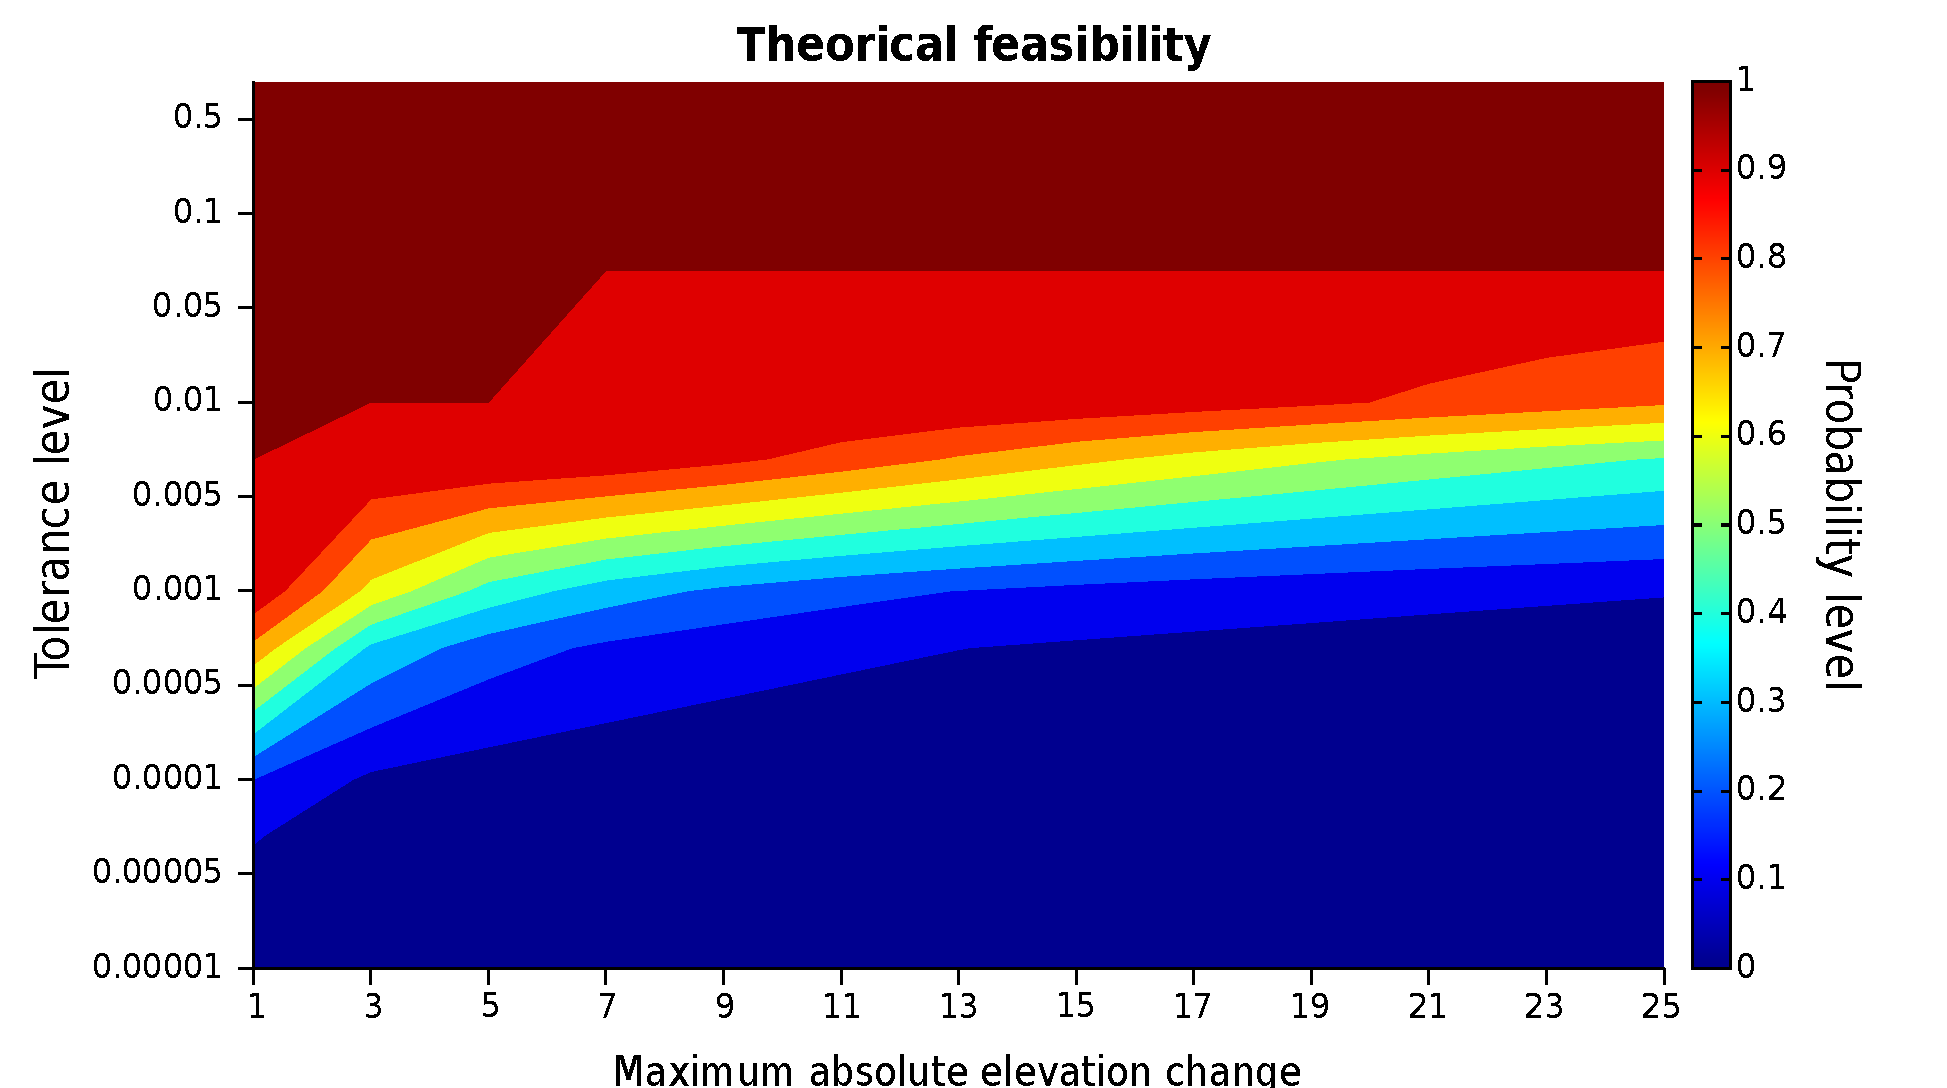
\includegraphics[width=\columnwidth]{Images/Technicalities/feasibilityNR51.pdf}  
\caption[Thing taken from our master thesis]{Thing taken from our master thesis whose meaning have been completely forgotten.}
\label{fig:massConstraintFeasibility}
\end{figure}

\begin{table}
\footnotesize
\centering
\begin{tabularx}{0.8\textwidth}{llrcl}
\toprule
\tableheadline{l}{Algorithm} &
\tableheadline{l}{Parameter} &
\tableheadlineMore{3}{c}{Suggested Values} \\
\midrule
\tablefirstcol{l}{Any}	& NFE	 		& $10\,000 $ 	& $ \div $ 	& $ 200\,000$ \\
				& Population Size 	&  $10 $ 		& $ \div $ 	& $ 1000$ \\
\midrule
\tablefirstcol{l}{GDE3} & DE step size 		& $0.0 $ 	& $\div $ 	& $ 1.0$ \\
				& Crossover rate 	& $0.0$ 	& $ \div $ 	& $ 1.0$ \\
\bottomrule
\end{tabularx}
\caption[Parameters needed for things]{Parameters needed for things that are not needed anymore themselves.}
\label{tab:MOEAandParameters}
\end{table}

\section{Contributing to this template}
Suggestion and improvements are welcome at \url{https://github.com/Lordmzn/ClassicThesis-at-DEIB} or via email at \url{emanuele.mason@polimi.it}, \url{andrea.cominola@polimi.it} or \url{daniela.anghileri@polimi.it}.
 
	\chapter{Stochastic Variance Reduced Policy Gradient} \label{chap:algorithm}
\vspace{-0.05in}
In online \acs{RL} problems, the usual approach is to manually tune the batch size of \acs{SG} to find the optimal trade-off between variance and speed.
Recall that, compared to \acs{SL}, the samples are not fixed in advance but we need to collect them at each policy update.
Since this operation may be costly, we would like to minimize the number of interactions with the environment.
For these reasons, we would like to apply \acs{SVRG} to \acs{RL} problems in order to limit the variance introduced by sampling trajectories, which would ultimately lead to faster convergence.
However, as previously introduced, a direct application of \acs{SVRG} to \acs{RL} is not possible due to the following issues:
% In on-line policy gradient problems, SG is not really a choice, but is dictated by the necessity of interacting with an unknown environment.\todopir{I do not understand the meaning of this sentence. I would say that SG is not a choice by referring to papers that use batches}
% We would like to apply SVRG to the policy gradient framework in order to limit the variance introduced by sampling trajectories, which would ultimately lead to faster convergence. In this scenario, the function $f(\vtheta)$ to optimize is $J(\vtheta)$ and the (implicit) dataset $\mathcal{D}$ is the set of all possible trajectories $\mathcal{T}$. Compared to the typical finite sum optimization scenario, we have the following additional challenges:
\begin{description}
	\item[\textbf{\MakeUppercase{N}on-concavity}:] the objective function $J(\vtheta)$ is typically non-concave for instance, in swimmer, a snake-like robot immersed in a fluid which must move forward we have: a 13-dimensional state space, 3 links velocities ($v_x$ and $v_y$ of center of masses) and 2 actuated joints angles. 2-dimensional action space which are the two momentums applied on the actuated joints. Therefore, the objective function will be:
	\[
	\ \int p_{\theta}(\tau)\mathcal{R}(\tau)d\tau
	\]
	with 
	\[
	\ \mathcal{R}(\tau) = \sum_{t=0}^{\infty}\gamma^t\mathcal{R}(s_t,a_t)
	\]
	and 
	\[
	\ \mathcal{R}(s_t,a_t)=v^t_x - 10^{-4}\norm[2]{a_t}^2
	\]
	\item[\textbf{\MakeUppercase{I}nfinite dataset}:] in continuous \acs{RL} tasks the \acs{RL} optimization cannot be expressed as a finite-sum problem. The objective function is an expected value over the trajectory density $p_{\vtheta}(\tau)$ of the total discounted reward, for which we would need an infinite dataset. Whereas in discrete \acs{RL} tasks, even though we can express the optimization problem as a finite-sum we can't handle it anyway because, due to combinatorial reasons, the number of addends appearing in the sum itself becomes easily intractable.
	%    \item[Approximation:] the dataset $\mathcal{T}$ can be infinite, but we can only sample a finite number of trajectories;
	\item[\textbf{\MakeUppercase{N}on-stationarity}:] the distribution of the samples changes over time. In particular, the value of the policy parameter $\vtheta$ influences the sampling process. More precisely, we need to resample after any update of the policy itself, which implies using different distributions to colect samples between different updates of the policy.
\end{description}
To deal with non-concavity, we require $J(\vtheta)$ to be $L$-smooth, which is a reasonable assumption for common policy classes such as Gaussian\footnote{See Section \ref{sec:gaussianassumption} in \hyperref[chap:convergence]{Chapter 4} for more details on the Gaussian policy case.} and softmax~\citep[\eg][]{Furmston2012unifying,pirotta2015lipschitz}.
Because of the infinite dataset, we can only rely on an estimate of the full gradient.
\citet{harikandeh2015stopwasting} analysed this scenario under the assumptions of $h$ being concave, showing that \acs{SVRG} is robust to an inexact computation of the full gradient. In particular, it is still possible to recover the original convergence rate if the error decreases at an appropriate speed. In \hyperref[chap:convergence]{Chapter 4} we will show how the estimation accuracy impacts on the convergence results with a non-concave objective.
Finally, the non-stationarity of the optimization problem introduces a bias into the \acs{SVRG} estimator in Eq.~\eqref{E:svrg.gradient.correction}.
To overcome the latter issue we employ importance weighting~\citep[\eg][]{rubinstein1981simulation,precup2000eligibility} to correct the distribution shift.
%Finally, we employ importance weighting~\citep[\eg]{rubinstein1981simulation,precup2000eligibility} to guarantee proper sampling of trajectories.


\begin{algorithm}[h]
	\caption{SVRPG}
	\label{alg:svrpg}
	\begin{algorithmic}[1]
		\STATE {\bfseries Input:} number of epochs $S$, epoch size $m$, step size $\alpha$, batch size $N$, mini-batch size $B$, gradient estimator $g$, initial parameter $\vtheta_{m}^0 := \wt{\vtheta}^0$
		\FOR{$s=0$ {\bfseries to} $S-1$}
		\STATE $\vtheta_0^{s+1} := \wt{\vtheta}^{s} = \vtheta_{m}^s$
		\STATE Sample $N$ trajectories $\{\tau_j\}$ from $p(\cdot\vert\wt{\vtheta}^{s})$
		\STATE $ \wt{\mu} = \gradApp{\wt{\vtheta}^{s}}{N}$ (see Eq.~\eqref{E:policygradient.estimate})% = \frac{1}{N}\sum_{j=0}^{N-1}g(\tau_j | \wt{\vtheta}^s)$
		\FOR{$t=0$ {\bfseries to} $m-1$}
		\STATE Sample $B$ trajectories $\{\tau_i\}$ from $p(\cdot\vert\vtheta_t^{s+1})$
		%        \STATE $c^{s+1}_t = \frac{1}{B} \sum\limits_{i=0}^{B-1} \left( g(\tau_i|\vtheta_t^{s+1}) - \omega(\tau_i|\vtheta^{s+1}_t, \wt{\vtheta}^s) g(\tau_i| \wt{\vtheta}^s) \right)$
		\STATE $c^{s+1}_t = \frac{1}{B} \sum\limits_{i=0}^{B-1}
		\begin{aligned}[t]
		\Big( & g(\tau_i|\vtheta_t^{s+1})\\ 
		& \quad{} - \omega(\tau_i|\vtheta^{s+1}_t, \wt{\vtheta}^s) g(\tau_i| \wt{\vtheta}^s) \Big)
		\end{aligned}$
		%        \STATE $\begin{aligned}[t]
		%                &v^{s+1}_t = \wt{\mu}\\ 
		%                & +\frac{1}{B} \sum\limits_{i=0}^{B-1} \left( g(\tau_i|\vtheta_t^{s+1}) - \omega(\tau_i|\vtheta^{s+1}_t, \wt{\vtheta}^s) g(\tau_i| \wt{\vtheta}^s) \right)
		%                \end{aligned}$
		\STATE $v^{s+1}_t = \wt{\mu} + c^{s+1}_t$ % \gradApp{\wt{\vtheta}^{s}}{N} + c^{s}_t$
		%%		\begin{align*}
		%%		\blacktriangledown J(\vtheta_t^{s+1}) = 
		%%		&\gradApp{\wt{\vtheta}^s}{N} \\
		%%		&+\frac{1}{B}\sum_{i=0}^{B-1}\left[ 
		%%		\score{}{\tau_i\vert\vtheta_t^{s+1}}\Reward(\tau_i)\right. \\
		%%		&\left. - \omega(\tau_i)\score{}{\tau_i \vert \wt{\vtheta}^{s}}\Reward(\tau_i)\right]
		%%		\end{align*}
		\STATE $\vtheta_{t+1}^{s+1} = \vtheta_t^{s+1} + \alpha v^{s+1}_t$
		\ENDFOR
		\ENDFOR
		\STATE {\bfseries return} $\vtheta_A\coloneqq\vtheta_t^{s+1}$ with $(s,t)$ picked uniformly at random from $\{[0,S-1]\times[0,m-1]\}$
	\end{algorithmic}
\end{algorithm} 

We can now introduce \acs{SVRPG} for a generic policy gradient estimator $g$ (\eg REINFORCE or G(PO)MDP). Pseudo-code is provided in Algorithm \ref{alg:svrpg}.
The overall structure is the same as Algorithm \ref{alg:svrg}, 
but the snapshot gradient is not exact and the gradient estimate used between snapshots is corrected using importance weighting:\footnote{Note that $g$ can be any unbiased estimator, with or without baseline. The unbiasedness is required for theoretical results.}
\begin{align*}
\blacktriangledown J(\vtheta_{t}) &= \wh{\nabla}_N J(\wt{\vtheta}) + g(\tau|\vtheta_t) - \omega(\tau|\vtheta_t, \wt{\vtheta}) g(\tau|\wt{\vtheta})
\end{align*}
for any $t \in \{0,\ldots,m-1\}$,
where $\wh{\nabla}_N J(\wt{\vtheta})$ is as in Eq.~\eqref{E:policygradient.estimate} where $\mathcal{D}_N$ is sampled using the snapshot policy $\pi_{\wt{\vtheta}}$, $\tau$ is sampled from the current policy $\pi_{\vtheta_t}$, and $\omega(\tau|\vtheta_t, \wt{\vtheta}) = \frac{p(\tau|\wt{\vtheta})}{p(\tau|\vtheta_t)}$ is an importance weight from $\pi_{\vtheta_t}$ to the snapshot policy $\pi_{\wt{\vtheta}}$. 
Similarly to \acs{SVRG}, we have that $\vtheta_0 := \wt{\vtheta}$, and the update is a \acs{FG} step.
Our update is still fundamentally on-policy since the weighting concerns only the correction term. However, this partial ``off-policyness'' represents an additional source of variance. This is a well-known issue of importance sampling~\citep[\eg][]{thomas2015high}. To mitigate it, we use mini-batches of trajectories of size $B \ll N$ to average the correction, \ie
\begin{align}\label{E:svrpg.estimate.batch}
\blacktriangledown J(\vtheta_{t}) &:= v_t= \wh{\nabla}_N J(\wt{\vtheta})\\ \notag
& \quad{} + 
\underbracket{
	\frac{1}{B} \sum_{i=0}^{B-1} \left[
	g(\tau_i|\vtheta_t) - \omega(\tau_i|\vtheta_t, \wt{\vtheta}) g(\tau_i|\wt{\vtheta})
	\right]}_{c_t}.
\end{align}
This gradient estimator is computed in Algorithm \ref{alg:svrpg} at lines 5, 7, 8 and 9.\newline
It is worth noting that the full gradient and the correction term have the same expected value:
\[
\ \EVV[\tau_i \sim p(\cdot|\vtheta_t)]{\frac{1}{B} \sum_{i=0}^{B-1} \omega(\tau_i|\vtheta_t, \wt{\vtheta}) g(\tau_i|\wt{\vtheta})} = \nabla J(\wt{\vtheta}).
\]
This property will be used to prove Lemma~\ref{L:svrpg.properties}. The reader can refer to \hyperref[chap:art]{Chapter 2} for off-policy gradients and variants of REINFORCE and G(PO)MDP.
%\begin{align*}
%&\blacktriangledown J(\vtheta) = \frac{1}{N}\sum_{j=0}^{N-1}\nabla\log\pi(\tau_j \vert \wt{\vtheta})\Reward(\tau_j) +\\
%&\quad\frac{1}{B}\left[\sum_{i=0}^{B-1}
%\nabla\log\pi(\tau_i \vert \vtheta)\Reward(\tau_i) 
%- \omega(\tau_i)\nabla\log\pi(\tau_i \vert \wt{\vtheta})\Reward(\tau_i)\right].
%\end{align*}
The use of mini-batches is also common practice in \acs{SVRG} since it can yield a performance improvement even in the supervised case~\citep{harikandeh2015stopwasting,konevcny2016mini}. It is easy to show that the \acs{SVRPG} estimator has the following, desirable properties:
\begin{lemma}\label{L:svrpg.properties}
	Let $\wh{\nabla}_N J(\vtheta)$ be an unbiased estimator of~\eqref{E:policygradient}
	%Denote by $\wh{\nabla}_N^{\textsc{RF}} J(\vtheta)$ the REINFORCE estimator in~\eqref{E:policygradient.estimate} 
	and let $\vtheta^* \in \argmin_{\vtheta} \{J(\vtheta)\}$. Then, the \acs{SVRG} estimate in~\eqref{E:svrpg.estimate.batch} is \emph{unbiased}
	\begin{equation}\label{eq:unbiased}
	\mathop{\mathbb{E}}
	\left[\blacktriangledown J(\vtheta)\right] = \gradJ{\vtheta}.
	\end{equation}
	and regardless of the mini-batch size $B$:
	\begin{equation}\label{eq:zerovar}
	\Var\left[\gradBlack{\vtheta^*}\right] = 
	\Var\left[\wh{\nabla}_N J(\vtheta^*)\right].
	\end{equation}
	For any vector $\mathbf{x}$, we use $\Var[\mathbf{x}]$ to denote the trace of the covariance matrix, \ie $\Tr\EVV[]{(\mathbf{x}-\EVV[]{\mathbf{x}})(\mathbf{x}-\EVV[]{\mathbf{x}})^T}$.
\end{lemma}
%\begin{proof}
%Claim (\ref{eq:unbiased}) is from the unbiasedness of the estimators:
%\begin{align*}
%\EVV[]{\gradBlack{\vtheta}} &= \EVV[]{\gradApp{\wt{\vtheta}}{N}}  + \EVV[]{\gradApp{\vtheta}{B}} \\
%&\qquad- \EVV[]{\frac{1}{B}\sum_{i=0}^{B-1}\omega(\tau_i|\vtheta, \wt{\vtheta}) g(\tau_i|\wt{\vtheta})} \\
%&= \gradJ{\wt{\vtheta}} + \gradJ{\vtheta} - \gradJ{\wt{\vtheta}} = \gradJ{\vtheta}.
%\end{align*}
%As for claim (\ref{eq:zerovar}), note that as $\vtheta\to\vtheta^*$, also $\wt{\vtheta}\to\vtheta^*$. Hence, by continuity of $J(\vtheta)$:
%\begin{align*}
%\Var\left[\gradBlack{\vtheta}\right] &\to \Var\left[\gradApp{\vtheta^*}{N}\right] + \frac{1}{B}\Var\left[g(\tau|\vtheta^*)\right. \\
%&\left.- \cancel{\omega(\tau|\vtheta^*,\vtheta^*)}g(\tau|\vtheta^*)\right]
%= \Var\left[\gradApp{\vtheta^*}{N}\right].
%\end{align*}
%Note that it is essential that the trajectories used in the second and the third term are the same for the variance to vanish.
%\end{proof}
Previous results hold for both REINFORCE and G(PO)MDP.
In particular, the latter result suggests that an \acs{SVRG}-like algorithm using $\gradBlack{\vtheta}$ can achieve faster convergence, by performing much more parameter updates with the same data without introducing additional variance (at least asymptotically).
Note that the randomized return value of Algorithm \ref{alg:svrpg} does not affect online learning at all, but will be used as a theoretical tool in the next chapter.

\vspace{-0.05in}
 
	\chapter{Convergence Guarantees of SVRPG} \label{chap:convergence}
In this chapter, we state the convergence guarantees for \acs{SVRPG}  with REINFORCE or G(PO)MDP gradient estimator.
We mainly leverage on the recent analysis of non-concave \acs{SVRG} (\cite{reddi2016stochastic,allen2016variance}).
As reported in Chapter \ref{chap:algorithm}, the direct application of \acs{SVRG} to \acs{RL} is not trivial due to the following issues: non-concavity, infinite dataset and non-stationarity.
Each of these challenges presented can potentially prevent convergence, so we need additional assumptions that we present in Section \ref{sec:assumption}. In Section \ref{sec:gaussianassumption} we show how Gaussian policies satisfy these assumptions. In Section \ref{sec:definition} we give some additional definitions which will be useful in the proofs. In Section \ref{sec:ancillarylemmas} we provide the ancillary lemmas for the convergence proof. In Section \ref{sec:maintheorem} we provide the statement and the proof of the convergence theorem. Finally in Section \ref{sec:consequence} we discuss the consequences of the convergence theorem.\newline
We state now the convergence guarantees for \acs{SVRPG}:

\begin{theorem}\label{theo:convergence}
	Assume the REINFORCE or the G(PO)MDP gradient estimator is used in SVRPG:
	\begin{align}
	\blacktriangledown J(\vtheta_{t}) &:= v_t= \wh{\nabla}_N J(\wt{\vtheta})\\ \notag
	& \quad{} + 
	\frac{1}{B} \sum_{i=0}^{B-1} \left[
	g(\tau_i|\vtheta_t) - \omega(\tau_i|\vtheta_t, \wt{\vtheta}) g(\tau_i|\wt{\vtheta})
	\right].
	\end{align}.
	Under Assumptions~\ref{ass:bounded_score}, \ref{ass:REINFORCE} and \ref{ass:M2}, the parameter vector $\vtheta_A$ returned by Algorithm~\ref{alg:svrpg} after $T=m\times S$ iterations has, for some positive constants $\psi,\zeta, \xi$ and for proper choice of the step size $\alpha$ and the epoch size $m$, the following property:
	\begin{align*}
	&\EVV[]
	{\norm[2]{\nabla J(\vtheta_A)}^2} 
	\leq
	\frac{J(\vtheta^*)-J(\vtheta_0)}{\psi T} +
	\frac{\zeta}{N}
	+\frac{\xi}{B},
	\end{align*}
	where $\psi,\zeta,\xi$ depend only on $\GRADLOG,\HESSLOG,\VARRF,\VARIS,\alpha$ and $m$.
\end{theorem}

\section{Assumptions}\label{sec:assumption}

As reported before we need additional assumptions for addressing the three issues of \acs{SVRG} applied to \acs{RL}:

\textit{1) Non-concavity.} A common assumption, in this case, is to assume the objective function to be $L$-smooth (\cite{reddi2016stochastic,allen2016variance}).
However, in \acs{RL} we can consider the following assumption which is sufficient for the $L$-smoothness of the objective (see Lemma~\ref{lemma:lsmooth}).

%assumtion
\begin{assumption}\label{ass:bounded_score}
	For each state-action pair $(s,a)$, any value of $\vtheta$, and all parameter components $i,j$ there exist constants $0 \leq G,F<\infty$ such that:
	\[
	\left|\nabla_{\theta_i}\log\pi_{\vtheta}(a\vert s)\right| \leq \GRADLOG, \qquad
	\left|\frac{\partial^2}{\partial\theta_i\partial\theta_j}\log\pi_{\vtheta}(a \vert s)\right| \leq \HESSLOG.
	\]
\end{assumption}

\textit{2) \acs{FG} Approximation.}
Since we cannot compute an exact full gradient due to the infinite dataset, we require the variance of the gradient estimator to be bounded.
This assumption is similar in spirit to the one in ~\cite{harikandeh2015stopwasting}.
\begin{assumption}\label{ass:REINFORCE}
	There is a constant $V<\infty$ such that, for any policy $\pol$:
	\[
	\Var\left[g(\cdot\vert\vtheta)\right] \leq \VARRF.
	\]
\end{assumption}

\textit{3) Non-stationarity.} 
Similarly to what done in \acs{SL} literature ~\citep{cortes2010learning}, we require the variance of the importance weight to be bounded.
\begin{assumption}\label{ass:M2}
	There is a constant $W<\infty$ such that, for each pair of policies encountered in Algorithm~\ref{alg:svrpg} and for each trajectory,
	\[
	\mathbb{V}ar\left[\omega(\tau| \vtheta_1, \vtheta_2)\right] \leq \VARIS, \quad \forall \vtheta_1,\vtheta_2 \in \realspace^d , \tau \sim p(\cdot|\vtheta_1).
	\]
\end{assumption}
Differently from Assumptions~\ref{ass:bounded_score} and ~\ref{ass:REINFORCE}, Assumption~\ref{ass:M2} must be enforced by a proper handling of the epoch size $m$.\newline
Given this assumptions, as shown in the next sections, we can handle the challenges and prove convergence guaranties of \acs{SVRPG}. Before that we need to give some definition and some lemma for a better  understanding of the final proof.

\section{Validity of assumptions for gaussian policies}\label{sec:gaussianassumption}
We can now provide more details on the applicability of convergence guarantees on the case of Gaussian policies. Gaussian policies are the most commonly policies in continuous RL applications, an example can be founded in \cite{kober2013reinforcement}. Gaussian policies are also used in our experiments, reported in Chapter \ref{chap:experiments}. We start by analyzing the case of one-dimensional bounded action space $\mathcal{A}\subset\mathbb{R}$, linear mean $\mu(s) = \vtheta^T\vphi(s)$ and fixed standard deviation $\sigma$, which corresponds to the following probability density function::
\[
\pi_{\vtheta}(a\vert s) = \frac{1}{\sqrt{2\pi}\sigma}\exp\left\{
-\frac{(\vtheta^T\vphi(s) - a)^2}{2\sigma^2}\right\},
\]
where $\vphi(s)\leq M_{\phi}$ is a bounded feature vector, and we see under which conditions the three assumptions of Section \ref{sec:assumption} hold.

For the Gaussian policy defined above, it's easy to show that:
\begin{align*}
&\nabla_{\theta_i}\log\pi_{\vtheta}(\tau) =  \phi_i(s)\frac{a-\vtheta^T\phi(s)}{\sigma^2},\\
&\frac{\partial^2}{\partial\theta_i\partial\theta_j}\log\pi_{\vtheta}(\tau) = \frac{\phi_i(s)\phi_j(s)}{\sigma^2}.
\end{align*}
Hence, Assumption \ref{ass:bounded_score} is automatically satisfied \footnote{This relies on the fact that $\vtheta^T\phi(s)$ lies in bounded $\Aspace$. In practice, this is usually enforced by clipping the action selected by $\pi_{\vtheta}$. A more rigorous way would be to employ the truncated Gaussian distribution or a squashing function.} by taking $\GRADLOG = \frac{M_{\phi}|\Aspace|}{\sigma^2}$ and $\HESSLOG = \frac{M_{\phi}^2}{\sigma^2}$.
\par

As mentioned, the work of \cite{pirotta2013adaptive} provides a bound on the variance of the REINFORCE estimator, adapted from \cite{zhao2011analysis}, which does not depend on $\vtheta$:
\begin{align*}
\Var\left[\gradApp{\theta_i}{N}\right] \leq \frac{R^2M_{\phi}^2H(1-\gamma^H)^2}{N\sigma^2(1-\gamma)^2}.
\end{align*}
The same authors provide a similar bound for G(PO)MDP:
\begin{align*}
\Var\left[\gradApp{\theta_i}{N}\right] \leq \frac{R^2M_{\phi}^2}{N\sigma^2(1-\gamma)^2}\left[
 \frac{1-\gamma^{2H}}{1-\gamma^2} + H\gamma^{2H} - 2\gamma^{2H}\frac{1-\gamma^{H}}{1-\gamma} \right].
\end{align*}
 So we can considered Assumption \ref{ass:REINFORCE} satisfied.


It is noted in \cite{cortes2010learning} that, for any two Gaussian distributions $\mathcal{N}(\mu_1,\sigma_1)$ and $\mathcal{N}(\mu_2,\sigma_2)$, the variance of the importance weights from the latter to the former is bounded whenever $\sigma_2 > \frac{\sqrt{2}}{2}\sigma_1$. This is automatically satisfied by our fixed-variance Gaussian policies, since $\sigma_2=\sigma_1=\sigma$.
We have demonstrated that the variance of importance weight is not infinite, by enforcing also that
$\mathbb{V}ar\left[\omega(\tau| \vtheta_1, \vtheta_2)\right] \leq \VARIS$ we need a proper handling of the epoch size $m$.
So, also Assumption \ref{ass:M2}, with proper handling of epoch size $m$, is been satisfied.


We now briefly examine some generalizations of the simple Gaussian policy defined above that can be found in applications. Note that all this variants are employed in our experiments and in particular are used almost always in real applications:

\paragraph{Multi-dimensional actions.}
When actions are \newline multi-dimensional, factored Gaussian policies are typically employed, so the results extend trivially from the one-dimensional case. 
Given an bounded action space $\mathcal{A}\subset\mathbb{R}^n$ such that each dimension is bounded: $a_i\leq|\Aspace|$, a state space $\mathcal{S}\subset\mathbb{R}^m$, linear mean $\mu(s) = \Theta\vphi(s)$, where $\Theta$  is an $mxn$ matrix, and fixed covariance matrix $\Sigma$, the multivariate normal distribution is:

\[
\pi_{\Theta}(a\vert s) = \frac{1}{\sqrt{2\pi\mid\Sigma\mid}}\exp\left\{
-\frac{1}{2}(a - \Theta\vphi(s))^T\Sigma^{-1}(a - \Theta\vphi(s))\right\},
\]

we show that:

\begin{align*}
&\nabla_{\Theta_{i,k}}\log\pi_{\Theta}(\tau) =  \phi_{i,k}(s)(a-\Theta\phi(s))\Sigma^{-1},\\
&\frac{\partial^2}{\partial\Theta_{i,k}\partial\Theta_{j,z}}\log\pi_{\Theta}(\tau) = \phi_{i,k}(s)\phi_{j,z}(s)\Sigma^{-1}.
\end{align*}

by taking $\GRADLOG = nM_{\phi}|\Aspace|\Sigma^{-1}$ and $\HESSLOG = M_{\phi}^2\Sigma^{-1}$ the assumption is satisfied.

\paragraph{Non-linear mean.}
In complex continuous tasks, $\mu(s)$ often represents a deep neural network, or multi-layer perceptron, where $\vtheta$ are the weights of the network. The analysis of first and second order log-derivatives in such a scenario is beyond the scope of this thesis.

\paragraph{Adaptive variance.}
It is a common practice to learn also the variance of the policy in order to adapt the degree of exploration. The variance (or diagonal covariance matrix in the multi-dimensional case) can be learned as a separate parameter or be state-dependent like the mean. In any case, adaptive variance must be carefully employed since it can clearly undermine all the three assumptions reported in Section  \ref{sec:assumption}.

\section{Definitions}\label{sec:definition}

We give some additional definitions which will be useful in the proofs.

\begin{definition}
	For a random variable X:
	\[
	\Es{X} = \EVV[\tau_j\sim\pi(\cdot\vert\wt{\vtheta}^s)
	\forall j\in\mathbf{N}]{X\vert\wt{\vtheta}^s},
	\]
	where $\wt{\vtheta}^s$ is defined in Algorithm \ref{alg:svrpg} and $\mathbf{N} = [0,\dots,N)$.
\end{definition}

We use the notation $\tau_{i,h}$ to denote the $h$-th trajectory collected using policy $\vtheta^{s+1}_i$ where $s$ is clear from the context.

\begin{definition}
	For a random variable $X$:
	\begin{align*}
	&\mathbb{E}_{t\vert s}\left[X\right] \coloneqq 
	\mathop{\mathbb{E}}_{\substack{\tau_j\sim\pi(\cdot\vert\wt{\vtheta}^s)\forall j \in N \\ \tau_{i,h}\sim\pi(\cdot\vert\vtheta^{s+1}_i) \forall h \in B, \text{ for $i=0,\dots,t$}}}{\left[X \vert \wt{\vtheta^s}\right]} \\
	&\coloneqq \EVV[\tau_j\sim\pi(\cdot\vert\wt{\vtheta}^s)\forall j \in N]{
		\EVV[\tau_{0,h}\sim\pi(\cdot\vert\vtheta_0^{s+1}) \forall h \in B]
		{\dots
			\EVV[\tau_{t,h}\sim\pi(\cdot\vert\vtheta_t^{s+1})\forall h \in B]
			{X\vert\vtheta_t^{s+1}}
			\dots
			\vert\vtheta_0^{s+1}}
		\vert\wt{\vtheta}^s}\\
	&= \EVV[t-1|s]{\EVV[\tau_{t,h}\sim \pi(\cdot|\vtheta^{s+1}_t)]{X|\vtheta^{s+1}_t}}
	\end{align*}
	where the sequence $\wt{\vtheta}^s,\vtheta_0^{s+1},\dots,\vtheta_t^{s+1}$ is defined in Algorithm \ref{alg:svrpg}, $\mathbf{N} = [0,\dots,N)$, and $\mathbf{B} = [0,\dots,B)$. To avoid inconsistencies, we also define $\Ets[(-1)]{X} \coloneqq \Es{X}$.
	
\end{definition}

Intuitively, the $\Ets{\cdot}$ operator computes the expected value with respect to the sampling of trajectories from the snapshot policy $\wt{\vtheta}^s$ up to the $t$-th iteration included. Note that the order in which expected values are taken is important since each $\vtheta_{t}^{s+1}$ is function of previously sampled trajectories and is used to sample new ones.
We want to point up that this is exactly the non-stationarity of the \acs{RL} problems: the trajectories sampled in a point have influence in all the point distributions of the future.

\begin{definition}\label{def:var}
	For random vectors X, Y:
	\begin{align*}
	\Covs{X}{Y} &\coloneqq \Tr\left(\Ets{(X-\Ets{X})(Y-\Ets{Y})^T}\right), \\
	\Vars{X} &\coloneqq \Covs{X}{Y},
	\end{align*}
	where $\Tr(\cdot)$ denotes the trace of a matrix. From the linearity of expected value we have the following:
	\begin{equation}\label{neweq:1}
	\Vars{X} = \Es{\norm[]{X-\Es{X}}^2}
	\end{equation}
	$\Covts[t]{X}{Y}$ and $\Varts[t]{X}$ are defined in the same way from $\Ets[t]{X}$.
\end{definition}
Note that we had to define the variance of vectors because there are a lot of vector variance definitions, this definition is that we  believe it is better for our calculations. 
\begin{definition}
	The full gradient estimation error is:
	\[
	e_s \coloneqq \gradApp{\wt{\vtheta}^s}{N} - \gradJ{\wt{\vtheta}^s} 
	\]
	and represent the difference between our estimate of gradient and the real gradient.
\end{definition}

\begin{definition}\label{def:ideal}
	The ideal \acs{SVRPG} gradient estimate is:
	\begin{align*}
	\gradIdeal{\vtheta_t^{s+1}} &\coloneqq 
	\gradJ{\wt{\vtheta}^s}
	%	+ \nabla\log\pi(\tau_i \vert \vtheta_t^{s+1})\Reward(\tau_i) 
	+ g(\tau_i|\vtheta^{s+1}_t)
	%	- \omega(\tau_i)\nabla\log\pi(\tau_i \vert \wt{\vtheta}^s)\Reward(\tau_i) 
	- \omega(\tau_i|\vtheta^{s+1}_t, \wt{\vtheta}^s) g(\tau_i|\wt{\vtheta}^s)
	\\
	&= \gradBlack{\vtheta_t^{s+1}} - \gradApp{\wt{\vtheta}^s}{N} + \gradJ{\wt{\vtheta}^s} \\
	&= \gradBlack{\vtheta_t^{s+1}} - e_s,
	\end{align*} and is the SVRPG gradient that we would use if the true value of the gradient was available.
\end{definition}


\section{Ancillary Lemmas}\label{sec:ancillarylemmas}

Before addressing the main convergence theorem, we prove some useful lemmas.


\begin{lemma}\label{lemma:lsmooth}
	Under Assumption \ref{ass:bounded_score}, $J(\vtheta)$ is L-smooth for some positive Lipschitz constant $L_J$.
\end{lemma}
\begin{proof}
	By definition of $J(\vtheta)$:
	\begin{align}
	\Dij{J(\vtheta)}{\theta} 
	&= \int_{\Tspace}\Dij{}{\theta}p(\tau|\vtheta)\Reward(\tau)\de \tau
	\nonumber\\ 
	&= \int_{\Tspace}p(\tau|\vtheta)\score{\vtheta}{\tau}\score{\vtheta}{\tau}^T\Reward(\tau)\de \tau\\ 
	&\qquad+ \int_{\Tspace}\pol(\tau)\Dij{}{\theta}\log p(\tau|\vtheta)\Reward(\tau)\de \tau \nonumber\\
	&\leq \sup_{\tau \in \mathcal{T}} \left\{\left|\Reward(\tau)\right|\right\} \left(H^2\GRADLOG^2+H\HESSLOG\right) \label{eq:0}\\
	&= \frac{1-\gamma^H}{1-\gamma}RH\left(H\GRADLOG^2+\HESSLOG\right),\nonumber
	\end{align}
	where Equation \ref{eq:0} is from Assumption \ref{ass:bounded_score} ($H$ represent the trajectories length: $\log p(\tau|\vtheta) = \sum_{t=0}^{M-1}\log\pi_{\vtheta}(a_t\vert s_t)$).
	Since the Hessian is bounded, $J(\vtheta)$ is Lipschitz-smooth.
\end{proof}

\begin{lemma}\label{lemma:gsmooth}
	Under Assumption \ref{ass:bounded_score}, whether we use the REINFORCE or the G(PO)MDP gradient estimator, $g(\tau\vert\vtheta)$ is Lipschitz continuous with Lipschitz constant $L_g$, \ie for any trajectory $\tau\in\Tspace$:
	\[
	\norm[2]{g(\tau\vert\vtheta)-g(\tau\vert\vtheta')}^2 \leq L_g\norm[2]{\vtheta-\vtheta'}^2.
	\]
\end{lemma}
\begin{proof}
	For both REINFORCE and G(PO)MDP, $g(\tau\vert\vtheta)$ is a linear combination of terms of the kind $\nabla \log \pi_{\vtheta}(a_t\vert s_t)\gamma^t r_t$ \citep{peters2008reinforcement}. These terms have bounded gradient from the second inequality of Assumption \ref{ass:bounded_score} and the fact that $|r_t|\leq R$. If a baseline is used in REINFORCE or G(PO)MDP, we only need the additional assumption that said baseline is bounded, which can always be assumed without compromising the correctness of the gradient estimatorm, since the choice of baseline is arbitrary.
	Bounded gradient implies Lipschitz continuity. Finally, the linear combination of Lipschitz continuous functions is Lipschitz continuous.
\end{proof}

\begin{lemma}\label{lemma:gbound}
	Under Assumption \ref{ass:bounded_score}, whether we use the REINFORCE or the G(PO)MDP gradient estimator, for every $\tau\in\Tspace$ and $\vtheta\in\Theta$, there is a positive constant $\Gamma<\infty$ such that:
	\[
	\norm[2]{g(\tau\vert\vtheta)}^2 \leq \Gamma.
	\]
\end{lemma}
\begin{proof}
	For REINFORCE we have, from Assumption \ref{ass:bounded_score}:
	\begin{align*}
	\norm[2]{g(\tau\vert\vtheta)}^2 &=
	\norm[2]{\score{\vtheta}{\tau}R(\tau)}^2 \\
	&=\norm[2]{\left(\sum_{t=0}^{H-1}\score{\vtheta}{a_t\vert s_t}\right)\left(\sum_{t=0}^{H-1}\gamma^t r_t\right)}^2 \\
	&\leq H^2G^2\frac{(1-\gamma^H)^2}{(1-\gamma)^2}R^2\dim(\vTheta) \coloneqq \Gamma
	\end{align*}
	For G(PO)MDP, we do not have a compact expression for $g$, but since it is derived from REINFORCE by neglecting some terms of the kind $\nabla \log \pi_{\vtheta}(a_t | s_t)\gamma^t r_t$ \citep{baxter2001infinite,peters2008reinforcement}, the above bound still holds.
	If a baseline is used in REINFORCE or G(PO)MDP, we only need the additional assumption that said baseline is bounded as reported before.
\end{proof}

%New Lemma on Variance
\begin{lemma}\label{lemma:varineq}
	For any random vector X, the variance (as defined in Definition \ref{def:var}), can be bounded as follows:
	\[
	\Vars{X} \leq \Es{\norm[]{X}^2}.
	\]
\end{lemma}
\begin{proof}
	By using basic properties of expected value and scalar variance:
	\begin{align*}
	\Vars{X} &= \Es{\norm[]{X-\Es{X}}^2} = \Es{\sum_{i=1}^{\dim(X)}\left(X_i-\Es{X_i}\right)^2}\\
	& = \sum_{i=1}^{\dim(X)}\Es{\left(X_i-\Es{X_i}\right)^2} \\
	&\leq \sum_{i=1}^{\dim(X)}\Es{X_i^2} = \Es{\sum_{i=1}^{\dim(X)}X_i^2} = \Es{\norm[]{X}^2}.
	\end{align*}
\end{proof}

%Lemma 2
\begin{lemma}\label{lemma:aux2}
	Under Assumption \ref{ass:bounded_score}
	, the expected squared norm of the \acs{SVRPG} gradient can be bounded as follows:
  \begin{align*}
	\Ets{\norm[2]{\gradBlack{\vtheta_t^{s+1}}}^2} \leq
	\Ets[t-1]{\norm[2]{\gradJ{\vtheta_t^{s+1}}}^2} 
	&+\frac{L_g^2}{B}\Ets[t-1]{\norm[2]{\vtheta_t^{s+1}-\wt{\vtheta}^s}^2}\\
	&+\frac{1}{N}\Vars{g(\cdot\vert\wt{\vtheta}^s)}
	\nonumber 
	+\frac{\Gamma\VARIS}{B}
	\end{align*}
\end{lemma}
\begin{proof}
	For ease of notation denote $\omega(\tau_i) := \omega(\tau_i|\vtheta^{s+1}_t, \wt{\vtheta}^{s})$. Then,
	\begingroup
	\allowdisplaybreaks
	\newgeometry{left=1cm,layouthoffset=-0.5cm,right=3cm,bottom=2cm,head=2cm}
	\begin{align}
	%            \Ets{\norm[2]{\gradBlack{\vtheta_t^{s+1}}}^2}
	&\mathbb{E}_{t|s}\big[\norm[2]{\gradBlack{\vtheta_t^{s+1}}}^2\big] = \Ets{\norm[]{\gradApp{\wt{\vtheta}^s}{N}
			+\frac{1}{B}\sum_{i=0}^{B-1} g(\tau_i\vert\vtheta_t^{s+1})
			-\frac{1}{B}\sum_{i=0}^{B-1}
			\omega(\tau_i)g(\tau_i\vert\wt{\vtheta}^s)}^2} \nonumber\\
	%
	&= \mathbb{E}_{t\vert s}\left[\left\|\gradApp{\wt{\vtheta}^s}{N}
	+\frac{1}{B}\sum_{i=0}^{B-1}\left( 
	g(\tau_i\vert\vtheta_t^{s+1}) -
	\omega(\tau_i)g(\tau_i\vert\wt{\vtheta}^s)\right)
	%\right.\right.\nonumber
	%\\&\qquad\left.\left.
	\pm \gradJ{\vtheta_t^{s+1}} \pm \gradJ{\wt{\vtheta}^s} 
	% -\gradJ{\vtheta_t^{s+1}} + \gradJ{\wt{\vtheta}^s}
	% +\gradJ{\vtheta_t^{s+1}} - \gradJ{\wt{\vtheta}^s}
	\right\|^2\right] \nonumber\\
	%
	&\leq \Ets[t-1]{\norm[]{\gradJ{\vtheta_t^{s+1}}}^2}
	+\Es{\norm[]{\gradApp{\wt{\vtheta}^s}{N} - \Es{\gradApp{\wt{\vtheta}^s}{N}}}^2} \nonumber\\
	&\qquad+ 
	\mathbb{E}_{t\vert s}\left[\left\|
	\frac{1}{B}\sum_{i=0}^{B-1}\left(
	g(\tau_i\vert\vtheta_t^{s+1}) -
	\omega(\tau_i)g(\tau_i\vert\wt{\vtheta}^s)\right)
	%	\right.\right.\nonumber\\&\qquad\left.\left.
	- \Ets{
		\frac{1}{B}\sum_{i=0}^{B-1}\left(
		g(\tau_i\vert\vtheta_t^{s+1}) -
		\omega(\tau_i)g(\tau_i\vert\wt{\vtheta}^s)\right)}\right\|^2\right] 
	\nonumber\\
	%
	&= \Ets[t-1]{\norm[]{\gradJ{\vtheta_t^{s+1}}}^2}
	+\Vars{\gradApp{\wt{\vtheta}^s}{N}} \nonumber\\
	&+ 
	\mathbb{E}_{t\vert s}\left[\left\|
	\frac{1}{B}\sum_{i=0}^{B-1}\left(
	g(\tau_i\vert\vtheta_t^{s+1}) -
	\omega(\tau_i)g(\tau_i\vert\wt{\vtheta}^s)\right)
	%	\right.\right.\nonumber\\&\qquad\left.\left.
	- \Ets{
		\frac{1}{B}\sum_{i=0}^{B-1}\left(
		g(\tau_i\vert\vtheta_t^{s+1}) -
		\omega(\tau_i)g(\tau_i\vert\wt{\vtheta}^s)\right)}\right\|^2\right] 
	\label{neweq:2}\\
	%
	&= \Ets[t-1]{\norm[]{\gradJ{\vtheta_t^{s+1}}}^2} 
	+\frac{1}{N}\Vars{g(\cdot\vert\wt{\vtheta}^s)}
	\nonumber\\
	&+ 
	\mathbb{E}_{t\vert s}\left[\left\|
	\frac{1}{B}\sum_{i=0}^{B-1}\left(
	g(\tau_i\vert\vtheta_t^{s+1}) -
	\omega(\tau_i)g(\tau_i\vert\wt{\vtheta}^s)\right)
%	 \right.\right.\nonumber\\&\qquad\left.\left.
	- \Ets{
		\frac{1}{B}\sum_{i=0}^{B-1}\left(
		g(\tau_i\vert\vtheta_t^{s+1}) -
		\omega(\tau_i)g(\tau_i\vert\wt{\vtheta}^s)\right)}\right\|^2\right] 
	\label{eq:1}\\%
	&\leq \Ets[t-1]{\norm[2]{\gradJ{\vtheta_t^{s+1}}}^2} 
	+\frac{1}{N}\Vars{g(\cdot\vert\wt{\vtheta}^s)} 
	+\Ets{\norm[2]{
			\frac{1}{B}\sum_{i=0}^{B-1}\left(
			g(\tau_i\vert\vtheta_t^{s+1}) -
			\omega(\tau_i)g(\tau_i\vert\wt{\vtheta}^s)\right)}^2} \label{eq:2}\\
	%
	&\leq \Ets[t-1]{\norm[2]{\gradJ{\vtheta_t^{s+1}}}^2} 
	+\frac{1}{N}\Vars{g(\cdot\vert\wt{\vtheta}^s)}
     \nonumber\\ 	&\qquad
	+ \frac{1}{B^2}\sum_{i=0}^{B-1}
	\Ets{\norm[2]{
			g(\tau_i\vert\vtheta_t^{s+1}) -
			\omega(\tau_i)g(\tau_i\vert\wt{\vtheta}^s) \pm g(\tau_i|\wt{\vtheta}^s) }^2} \nonumber\\
	&\leq \Ets[t-1]{\norm[]{\gradJ{\vtheta_t^{s+1}}}^2} 
	+\frac{1}{N}\Vars{g(\cdot\vert\wt{\vtheta}^s)}
	\nonumber\\
	&\qquad+
	\frac{1}{B^2}\sum_{i=0}^{B-1}
	\Ets{\norm[]{g(\tau_i\vert\vtheta_t^{s+1})
			-g(\tau_i\vert\wt{\vtheta}^s)}^2} 
%         \nonumber\\ 	&\qquad
	+\frac{1}{B^2}\sum_{i=0}^{B-1}
	\Ets{\norm[]{g(\tau_i\vert\wt{\vtheta}^s) 
			-\omega(\tau_i)g(\tau_i\vert\wt{\vtheta}^s)}^2} \nonumber\\
	%
	&\leq \Ets[t-1]{\norm[]{\gradJ{\vtheta_t^{s+1}}}^2} 
	+\frac{1}{N}\Vars{g(\cdot\vert\wt{\vtheta}^s)}
	\nonumber\\
	&\qquad
	+\frac{L_g^2}{B}\Ets[t-1]{\norm[]{\vtheta_t^{s+1}-\wt{\vtheta}^s}^2}
	+
	\frac{1}{B^2}\sum_{i=0}^{B-1}
	\Ets{\norm[]{(1 
			-\omega(\tau_i))g(\tau_i\vert\wt{\vtheta}^s)}^2} \label{eq:3}\\
	% ...
	%\end{align*}
	%\begin{align}
	% ...
	&\leq \Ets[t-1]{\norm[]{\gradJ{\vtheta_t^{s+1}}}^2} 
	+\frac{1}{N}\Vars{g(\cdot\vert\wt{\vtheta}^s)}
	\nonumber\\
	&\qquad+\frac{L_g^2}{B}\Ets[t-1]{\norm[]{\vtheta_t^{s+1}-\wt{\vtheta}^s}^2}
	+\Gamma\frac{1}{B^2}\sum_{i=0}^{B-1}\Ets{(\omega(\tau_i)-1)^2} \label{eq:4}\\
	%
	&= \Ets[t-1]{\norm[]{\gradJ{\vtheta_t^{s+1}}}^2} 
	+\frac{1}{N}\Vars{g(\cdot\vert\wt{\vtheta}^s)}
	\nonumber\\&\qquad
	+\frac{L_g^2}{B}\Ets[t-1]{\norm[]{\vtheta_t^{s+1}-\wt{\vtheta}^s}^2}
	+\frac{\Gamma}{B^2}\sum_{i=0}^{B-1}\Varts{\omega(\tau_i)} \nonumber\\
	%
	&\leq \Ets[t-1]{\norm[]{\gradJ{\vtheta_t^{s+1}}}^2} 
	+\frac{1}{N}\Vars{g(\cdot\vert\wt{\vtheta}^s)}
%	\nonumber\\ &\qquad
	+\frac{L_g^2}{B}\Ets[t-1]{\norm[]{\vtheta_t^{s+1}-\wt{\vtheta}^s}^2}
	+\frac{\Gamma\VARIS}{B}, \label{eq:5}
	\end{align}
	\restoregeometry
	\endgroup
	where (\ref{neweq:2}) is from (\ref{neweq:1}), (\ref{eq:1}) is from the definition of $\gradApp{\vtheta}{N}$, (\ref{eq:2}) is from Lemma \ref{lemma:varineq}, (\ref{eq:3}) is from Lemma \ref{lemma:gsmooth}, 
	(\ref{eq:4}) is from Lemma \ref{lemma:gbound}, and (\ref{eq:5}) is from Assumption \ref{ass:M2}.
\end{proof}

%Lemma 0
\begin{lemma}\label{lemma:aux0}
	Under Assumption \ref{ass:bounded_score}, for any function $\varphi(\vtheta_t^{s+1})$ which is deterministic for a fixed $\vtheta_t^{s+1}$:
	\begin{align*}
	\left|\Ets[t]{\dotprod{\gradBlack{\vtheta_t^{s+1}}}{\varphi(\vtheta_t^{s+1})}}
	-\Ets{\dotprod{\gradJ{\vtheta_t^{s+1}}}{\varphi(\vtheta_t^{s+1})}}
	\right| \\
	\leq
	\frac{1}{2N}\Vars{g(\cdot\vert\wt{\vtheta}^s)} +\frac{1}{2}\Ets[t-1]{\norm[]{\varphi(\vtheta_t^{s+1})}^2}
	\end{align*}
\end{lemma}
\begin{proof}
	\begin{align}
	&\Ets{\dotprod{\gradBlack{\vtheta_t^{s+1}}}{\varphi(\vtheta_t^{s+1})}}\\
	&=\Ets{\dotprod{\gradIdeal{\vtheta_t^{s+1}}}{\varphi(\vtheta_t^{s+1})}} 
	+ \Ets[t-1]{\dotprod{e_s}{\varphi(\vtheta_t^{s+1})}} \label{eq:6}\\
	&=\Ets{\dotprod{\gradJ{\vtheta_t^{s+1}}}{\varphi(\vtheta_t^{s+1})}} 
	+ \Ets[t-1]{\dotprod{e_s}{\varphi(\vtheta_t^{s+1})}} \label{eq:7}\\
	&= \Ets{\dotprod{\gradJ{\vtheta_t^{s+1}}}{\varphi(\vtheta_t^{s+1})}} 
	+\dotprod{\Ets{e_s}}{\Ets{\varphi(\vtheta_t^{s+1})}}\nonumber\\
	&\qquad+\Covts[t-1]{\gradApp{\wt{\vtheta}^s}{N}}{\varphi(\vtheta_t^{s+1})}  \label{eq:new1}\\
	&= 
	\Ets{\dotprod{\gradJ{\vtheta_t^{s+1}}}{\varphi(\vtheta_t^{s+1})}} +
	\Covts[t-1]{\gradApp{\wt{\vtheta}^s}{N}}{\varphi(\vtheta_t^{s+1})} \label{eq:8}
	\end{align}
	where~\eqref{eq:6} is from Definition~\ref{def:ideal};~\eqref{eq:7} is from the fact that $\gradIdeal{\vtheta_t^{s+1}}$ is both unbiased and independent from $\varphi(\vtheta_t^{s+1})$ \wrt the sampling at time $t$ alone, which is not true for $\gradBlack{\vtheta_t^{s+1}}$;~\eqref{eq:new1} is from the fact that $\gradJ{\wt{\vtheta}^s}$ is constant \wrt $\Vars{\cdot}$;~\eqref{eq:8} is from $\Ets{e_s}=0$.
	Hence:
	\begin{align}
	\left|\Ets{\dotprod{\gradBlack{\vtheta_t^{s+1}}}{\varphi(\vtheta_t^{s+1})}}
	\right.&-\left.\Ets{\dotprod{\gradJ{\vtheta_t^{s+1}}}{\varphi(\vtheta_t^{s+1})}}\right|  \\
	&=
	\left|\Covts[t-1]{\gradApp{\wt{\vtheta}^s}{N}}{\varphi(\vtheta_t^{s+1})}\right|  
	\nonumber\\
	&\leq
	\sqrt{\Vars{\gradApp{\wt{\vtheta}^s}{N}}} \cdot \sqrt{\Varts[t-1]{\varphi(\vtheta_t^{s+1})}} \label{eq:9a}\\
	%
	&\leq	
	\frac{1}{2}\Vars{\gradApp{\wt{\vtheta}^s}{N}} +\frac{1}{2}\Varts[t-1]{\varphi(\vtheta_t^{s+1})}\label{eq:9}\\
	%
	&=
	\frac{1}{2N}\Vars{g(\cdot\vert\wt{\vtheta}^s)} +\frac{1}{2}\Varts[t-1]{\varphi(\vtheta_t^{s+1})} \label{eq:10}\\
	%
	&\leq
	\frac{1}{2N}\Vars{g(\cdot\vert\wt{\vtheta}^s)} +\frac{1}{2}\Ets[t-1]{\norm[]{\varphi(\vtheta_t^{s+1})}^2},
	\label{neweq:3}
	\end{align}
	where~\eqref{eq:9a} comes from Cauchy-Schwarz inequality
	\begin{align}
	|\Cov(X,Y)| = |\EVV[]{(X-\mu_X)\transpose{(Y-\mu_Y)}}|.& \leq \EVV[]{(X-\mu_X)^2}^{1/2}\EVV[]{(Y-\mu_Y)^2}^{1/2}  \\
	& = \sqrt{\Var(X) \Var(Y)},
	\end{align}
	\eqref{eq:9} is from Young's inequality,~\eqref{eq:10} is from the definition of $\gradApp{\vtheta}{N}$, and \eqref{neweq:3} is from Lemma \ref{lemma:varineq}.
\end{proof}

%Lemma 1
\begin{lemma}\label{lemma:aux1}
	Under Assumptions \ref{ass:bounded_score} ans \ref{ass:M2}, the expected squared norm of the true gradient $\gradJ{\vtheta_t^{s+1}}$, for appropriate choices of $\alpha_t\geq0$ and $\beta_t>0$, can be bounded as follows:
	\[
	\Ets[t-1]{\norm[]{\gradJ{\vtheta_t^{s+1}}}^2} \leq
	\frac{R_{t+1}^{s+1} - R_t^{s+1}}{\Psi_t} + \frac{d_tV}{N\Psi_t}
	+\frac{f_tW}{B\Psi_t},
	\]
	where
	\begin{align*}
	&R_t^{s+1}\coloneqq \Ets[t-1]{J(\vtheta_t^{s+1}) - c_t\norm[]{\vtheta_t^{s+1}-\wt{\vtheta}^s}^2}, \\
	&c_{m} = 0, \\
	&c_t = c_{t+1}\left(1+\alpha_t\beta_t+\alpha_t+\frac{\alpha_t^2L^2}{B}\right)+\frac{\alpha_t^2L^3}{2B}, \\
	&\Psi_t = \alpha_t\left(\frac{1}{2}-\frac{c_{t+1}}{\beta_t}-\frac{\alpha_tL}{2}-\alpha_tc_{t+1}\right), \\
	&d_t = \frac{\alpha_t}{2}\left(1+2c_{t+1}+\alpha_tL+2\alpha_tc_{t+1}\right), \\
	&f_t = \alpha_t^2\frac{\Gamma(L+2c_{t+1})}{2},
	\end{align*}
	where $L=\max\left\{L_J,L_g\right\}$, \ie the greater of the Lipschitz constants from Lemmas \ref{lemma:lsmooth} and \ref{lemma:gsmooth}.
	
	In particular, the following constraints on $\alpha_t$ and $\beta_t$ are sufficient:
	\begin{align*}
	&0\leq\alpha_t < \frac{1-\nicefrac{2c_{t+1}}{\beta_t}}{L+2c_{t+1}} \\
	&\beta_t > 2c_{t+1}.
	\end{align*}
\end{lemma}
\begin{proof}
	We have:
	\begin{align}
	\Ets{J(\vtheta_{t+1}^{s+1})} 
	&\geq \Ets{J(\vtheta_t^{s+1})+\dotprod{\gradJ{\vtheta_t^{s+1}}}{\vtheta_{t+1}^{s+1}-\vtheta_t^{s+1}} - \frac{L}{2}\norm[]{\vtheta_{t+1}^{s+1}-\vtheta_t^{s+1}}^2} \label{eq:11}\\
	&= \Ets{J(\vtheta_t^{s+1})+\alpha_t\dotprod{\gradJ{\vtheta_t^{s+1}}}{\gradBlack{\vtheta_t^{s+1}}} - \frac{\alpha_t^2L}{2}\norm[]{\gradBlack{\vtheta_t^{s+1}}}^2} \label{eq:12}\\
	&\geq
	\Ets{J(\vtheta_t^{s+1})+\alpha_t\norm[]{\gradJ{\vtheta_t^{s+1}}}^2 - \frac{\alpha_t^2L}{2}\norm[]{\gradBlack{\vtheta_t^{s+1}}}^2} \nonumber\\
	&\qquad-
	\frac{\alpha_t}{2N}\Vars{g(\cdot\vert\wt{\vtheta}^s)} -\frac{\alpha_t}{2}\Ets[t-1]{\norm[]{\gradJ{\vtheta_t^{s+1}}}^2}, \label{eq:13}
	\end{align}
	where~\eqref{eq:11} is from the L-smoothness of $J(\vtheta)$ \citep{nesterov2013introductory} and \eqref{eq:12} is from the \acs{SVRPG} update.
	Inequality~\ref{eq:13} follows from Lemma~\ref{lemma:aux0} by noticing that $\nabla J(\vtheta^{s+1}_t)$ is a deterministic function given $\vtheta^{s+1}_t$. As a consequence, we can directly apply Lemma~\ref{lemma:aux0} with $\vphi(\vtheta_t^{s+1})\coloneqq\gradJ{\vtheta_t^{s+1}}$.
	
	Next, we have:
	\begingroup
	\allowdisplaybreaks
	\begin{align}
	\mathbb{E}_{t|s}\bigg[ & \norm[]{\vtheta_{t+1}^{s+1}-\wt{\vtheta}^s}^2 \bigg]
	= \Ets{\norm[]{\vtheta_{t+1}^{s+1}- \vtheta_t^{s+1} + \vtheta_t^{s+1}-\wt{\vtheta}^s}^2} \nonumber\\
	&=\Ets{\norm[]{\vtheta_{t+1}^{s+1}-\vtheta_{t}^{s+1}}^2+\norm[]{\vtheta_t^{s+1}-\wt{\vtheta}^s}^2+2\dotprod{\vtheta_{t+1}^{s+1}-\vtheta_{t}^{s+1}}{\vtheta_t^{s+1}-\wt{\vtheta}^s}} \label{eq:14a} \\
	&= \Ets{\alpha_t^2\norm[]{\gradBlack{\vtheta_t^{s+1}}}^2+\norm[]{\vtheta_t^{s+1}-\wt{\vtheta}^s}^2+2\alpha_t\dotprod{\gradBlack{\vtheta_t^{s+1}}}{\vtheta_t^{s+1}-\wt{\vtheta}^s}} \label{eq:14}\\
	&\leq \Ets{\alpha_t^2\norm[]{\gradBlack{\vtheta_t^{s+1}}}^2+\norm[]{\vtheta_t^{s+1}-\wt{\vtheta}^s}^2+2\alpha_t\dotprod{\gradJ{\vtheta_t^{s+1}}}{\vtheta_t^{s+1}-\wt{\vtheta}^s}} \nonumber\\ 
	&\qquad+
	\frac{\alpha_t}{N}\Vars{g(\cdot\vert\wt{\vtheta}^s)} +\alpha_t\Ets[t-1]{\norm[]{\vtheta_t^{s+1}-\wt{\vtheta}^s}^2} \label{eq:15}\\
	%
	&\leq \Ets{\alpha_t^2\norm[]{\gradBlack{\vtheta_t^{s+1}}}^2+\norm[]{\vtheta_t^{s+1}-\wt{\vtheta}^s}^2}\nonumber\\
	&\qquad+2\alpha_t\Ets[t-1]{\left|\dotprod{\gradJ{\vtheta_t^{s+1}}}{\vtheta_t^{s+1}-\wt{\vtheta}^s}\right|} \nonumber\\ 
	&\qquad+
	\frac{\alpha_t}{N}\Vars{g(\cdot\vert\wt{\vtheta}^s)} +\alpha_t\Ets[t-1]{\norm[]{\vtheta_t^{s+1}-\wt{\vtheta}^s}^2} \nonumber\\
	%
	&\leq \Ets{\alpha_t^2\norm[]{\gradBlack{\vtheta_t^{s+1}}}^2+\norm[]{\vtheta_t^{s+1}-\wt{\vtheta}^s}^2}\nonumber\\
	&\qquad+2\alpha_t\Ets[t-1]{\norm[]{\gradJ{\vtheta_t^{s+1}}}\norm[]{\vtheta_t^{s+1}-\wt{\vtheta}^s}} \nonumber\\ 
	&\qquad+
	\frac{\alpha_t}{N}\Vars{g(\cdot\vert\wt{\vtheta}^s)} +\alpha_t\Ets[t-1]{\norm[]{\vtheta_t^{s+1}-\wt{\vtheta}^s}^2} \nonumber\\
	%
	&\leq \Ets{\alpha_t^2\norm[]{\gradBlack{\vtheta_t^{s+1}}}^2+\norm[]{\vtheta_t^{s+1}-\wt{\vtheta}^s}^2}\nonumber\\ 
	&+2\alpha_t\Ets[t-1]{\frac{1}{2\beta_t}\norm[]{\gradJ{\vtheta_t^{s+1}}}^2+\frac{\beta_t}{2}\norm[]{\vtheta_t^{s+1}-\wt{\vtheta}^s}^2} \label{eq:16a}\\ 
	&\qquad
	+\frac{\alpha_t}{N}\Vars{g(\cdot\vert\wt{\vtheta}^s)} +\alpha_t\Ets[t-1]{\norm[]{\vtheta_t^{s+1}-\wt{\vtheta}^s}^2}, \label{eq:16}
	\end{align}
	\endgroup
	where~\eqref{eq:14a} is obtained using the triangular inequality,~\eqref{eq:14} is from the \acs{SVRPG} update,~\eqref{eq:15} is from Lemma~\ref{lemma:aux0} with\newline $\vphi(\vtheta_t^{s+1})\coloneqq\vtheta_t^{s+1}-\tilde{\vtheta}^s$,~\eqref{eq:16a} is from Cauchy-Schwarz inequality, and~\eqref{eq:16} is from Young's inequality in the `Peter-Paul' variant.
	Let us consider the following function:
	\begin{equation}\label{E:lyapunov.function}
	R_{t+1}^{s+1} \coloneqq \Ets{J(\vtheta_{t+1}^{s+1}) - c_{t+1}\norm[]{\vtheta_{t+1}^{s+1}-\tilde{\vtheta}^s}^2}. 
	\end{equation}
	The objective is now to provide a lower bound to it.
	\begingroup
	\allowdisplaybreaks
	\begin{align}
	&R_{t+1}^{s+1} 
	\geq	\Ets{J(\vtheta_t^{s+1}) - \frac{\alpha_t^2L}{2}\norm[]{\gradBlack{\vtheta_t^{s+1}}}^2}
	+ \EVV[t-1|s]{\frac{\alpha_t}{2}\norm[]{\gradJ{\vtheta_t^{s+1}}}^2}
	\nonumber\\
	&\qquad-
	\frac{\alpha_t}{2N}\Vars{g(\cdot\vert\tilde{\vtheta}^s)}
	-c_{t+1}\Ets{\norm[]{\vtheta_{t+1}^{s+1}-\tilde{\vtheta}^s}^2} \label{eq:17}\\
	%
	&\geq \Ets{J(\vtheta_t^{s+1}) - \frac{\alpha_t^2L}{2}\norm[]{\gradBlack{\vtheta_t^{s+1}}}^2}\\
	&\qquad+ \Ets[t-1]{\frac{\alpha_t}{2}\norm[]{\gradJ{\vtheta_t^{s+1}}}^2 }
	-\frac{\alpha_t}{2N}\Vars{g(\cdot\vert\tilde{\vtheta}^s)} \nonumber\\
	&\qquad -c_{t+1}\Ets{\alpha_t^2\norm[]{\gradBlack{\vtheta_t^{s+1}}}^2+\norm[]{\vtheta_t^{s+1}-\tilde{\vtheta}^s}^2}
	\nonumber\\
	&\qquad-2c_{t+1}\alpha_t\Ets[t-1]{\frac{1}{2\beta_t}\norm[]{\gradJ{\vtheta_t^{s+1}}}^2+\frac{\beta_t}{2}\norm[]{\vtheta_t^{s+1}-\tilde{\vtheta}^s}^2} \nonumber\\ 
	&\qquad
	-c_{t+1}\frac{\alpha_t}{N}\Vars{g(\cdot\vert\tilde{\vtheta}^s)} -c_{t+1}\alpha_t\Ets[t-1]{\norm[]{\vtheta_t^{s+1}-\tilde{\vtheta}^s}^2} \label{eq:18}\\
	%
	&= \Ets[t-1]{J(\vtheta_t^{s+1})} - c_{t+1}\left(1+\alpha_t\beta_t+\alpha_t\right)\Ets[t-1]{\norm[]{\vtheta_{t}^{s+1}-\tilde{\vtheta}}^2} \nonumber\\
	&\qquad-\alpha_t^2\left(\frac{L}{2}+c_{t+1}\right)\Ets{\norm[]{\gradBlack{\vtheta_t^{s+1}}}^2}\nonumber\\ &\qquad+\frac{\alpha_t}{2}\left(1-\frac{2c_{t+1}}{\beta_t}\right)\Ets[t-1]{\norm[]{\gradJ{\vtheta_t^{s+1}}}^2} \nonumber\\
	&\qquad-\frac{\alpha_t}{2N}\left(1+2c_{t+1}\right)\Vars{g(\cdot\vert\tilde{\vtheta}^s)} \nonumber\\
	%
	&\geq  \Ets[t-1]{J(\vtheta_t^{s+1})} - c_{t+1}\left(1+\alpha_t\beta_t+\alpha_t\right)\Ets[t-1]{\norm[]{\vtheta_{t}^{s+1}-\tilde{\vtheta}}^2} \nonumber\\
	&\qquad
	-\alpha_t^2\left(\frac{L}{2}+c_{t+1}\right)\left(\Ets[t-1]{\norm[]{\gradJ{\vtheta_t^{s+1}}}^2} 
	+\frac{1}{N}\Vars{g(\cdot\vert\tilde{\vtheta}^s)}
	\right.\nonumber\\
	&\left.\qquad+\frac{L^2}{B}\Ets[t-1]{\norm[]{\vtheta_t^{s+1}-\tilde{\vtheta}^s}^2}
	+\frac{\Gamma W}{B}\right)\nonumber\\
	&\qquad+\frac{\alpha_t}{2}\left(1-2\frac{c_{t+1}}{\beta_t}\right)\Ets[t-1]{\norm[]{\gradJ{\vtheta_t^{s+1}}}^2} -\frac{\alpha_t}{2N}\left(1+2c_{t+1}\right)\Vars{g(\cdot\vert\tilde{\vtheta}^s)} \label{eq:19}\\
	%
	& = \Ets[t-1]{J(\vtheta_t^{s+1}) - \left(c_{t+1}\left(1+\alpha_t\beta_t+\alpha_t+\frac{\alpha_t^2L^2}{B}\right)+\frac{\alpha_t^2L^3}{2B}\right)\norm[]{\vtheta_{t}^{s+1}-\tilde{\vtheta}}^2} \nonumber\\
	&\qquad
	+\alpha_t\left(\frac{1}{2}-\frac{c_{t+1}}{\beta_t}-\frac{\alpha_tL}{2}-\alpha_tc_{t+1}\right)\Ets[t-1]{\norm[]{\gradJ{\vtheta_t^{s+1}}}^2} \nonumber\\
	&\qquad-\frac{\alpha_t}{2N}\left(1+2c_{t+1}+\alpha_tL+2\alpha_tc_{t+1}\right)\Vars{g(\cdot\vert\tilde{\vtheta}^s)} 
	%    \nonumber\\ &\qquad
	-\alpha_t^2\frac{(L+2c_{t+1})\Gamma\VARIS}{2B} \nonumber\\
	%
	&= R_t^{s+1}
	+\Psi_t\Ets[t-1]{\norm[]{\gradJ{\vtheta_t^{s+1}}}^2}
	-\frac{d_t}{N}\Vars{g(\cdot\vert\tilde{\vtheta}^s)}
	-\frac{f_t}{B}\VARIS,\nonumber\\
	&\geq R_t^{s+1}
	+\Psi_t\Ets[t-1]{\norm[]{\gradJ{\vtheta_t^{s+1}}}^2}
	-\frac{d_t}{N}\VARRF
	-\frac{f_t}{B}\VARIS, \label{eq:20}
	\end{align}
	\endgroup
	where~\eqref{eq:17} is from~\eqref{eq:13} noticing that \newline $\EVV[t|s]{\norm[]{\nabla J(\vtheta^{s+1}_t)}^2} = \EVV[t-1|s]{\norm[]{\nabla J(\vtheta^{s+1}_t)}^2}$,~\eqref{eq:18} is from~\eqref{eq:16},~\eqref{eq:19} is from Lemma~\ref{lemma:aux2}, and (\ref{eq:20}) is from Assumption \ref{ass:REINFORCE}.
	To complete the proof, besides rearranging terms, we have to ensure that $\Psi_t>0$ for each $t$. This gives the constraints on $\alpha_t$ and $\beta_t$.
\end{proof}


\section{Main theorem}\label{sec:maintheorem}

We finally provide the proof of the convergence theorem:

\begin{theorem}\label{theo:convergence2}
	Assume the REINFORCE or the G(PO)MDP gradient estimator is used in SVRPG:
	\begin{align}
	\blacktriangledown J(\vtheta_{t}) &:= v_t= \wh{\nabla}_N J(\wt{\vtheta})\\ \notag
	& \quad{} + 
		\frac{1}{B} \sum_{i=0}^{B-1} \left[
		g(\tau_i|\vtheta_t) - \omega(\tau_i|\vtheta_t, \wt{\vtheta}) g(\tau_i|\wt{\vtheta})
		\right].
	\end{align}
	then, under Assumptions~\ref{ass:bounded_score}, \ref{ass:REINFORCE} and \ref{ass:M2}, the parameter vector $\vtheta_A$ returned by Algorithm~\ref{alg:svrpg} after $T=m\times S$ iterations has, for some positive constants $\psi,\zeta, \xi$ and for proper choice of the step size $\alpha$ and the epoch size $m$, the following property:
	\begin{align*}
	&\EVV[]
	{\norm[2]{\nabla J(\vtheta_A)}^2} 
	\leq
	\frac{J(\vtheta^*)-J(\vtheta_0)}{\psi T} +
	\frac{\zeta}{N}
	+\frac{\xi}{B},
	\end{align*}
	where $\psi,\zeta,\xi$ depend only on $\GRADLOG,\HESSLOG,\VARRF,\VARIS,\alpha$ and $m$.
\end{theorem}
\begin{proof}
	We prove the theorem for the following values of the constants:
	\begin{align*}
	& \psi \coloneqq \min_t\{\Psi_t\}, 
	& \zeta \coloneqq \frac{\max_t\{d_t\}V}{\psi}, 
	&& \xi \coloneqq \frac{\max_t\{f_t\}W}{\psi},
	\end{align*}
	where $\Psi$, $d_t$ and $f_t$ are defined in Lemma~\ref{lemma:aux1}.
	% The values of all other constants and the constraints on the step size are provided in Lemma \ref{lemma:aux1}.
	Starting from Lemma \ref{lemma:aux1}, summing over iterations of an epoch $s$ and using telescopic sum we obtain
	\begin{align*}
	\sum_{t=0}^{m-1}\Ets{\norm[]{\gradJ{(\vtheta_t^{s+1})}^2}}&\leq
	\frac{\sum_{t=0}^{m-1}\left(R_{t+1}^{s+1} - R_t^{s+1}\right)}{\psi} + \frac{m\zeta}{N} + \frac{m\xi}{B} \nonumber\\
	& = \frac{R^{s+1}_m - R^{s+1}_0}{\psi}  + \frac{m\zeta}{N} + \frac{m\xi}{B}
	\end{align*}
	By using the definition of $R^s_t$ in~\eqref{E:lyapunov.function}, the fact that $c_m = 0$ and $\vtheta^{s+1}_0 = \wt{\vtheta}^s = \vtheta^s_m$, we can state that:
	\begin{align*}
	R^{s+1}_m - &R^{s+1}_0 \\
	& = \EVV[m|s]{J(\vtheta^{s+1}_{m})- c_m \norm[]{\vtheta^{s+1}_{m} - \wt{\vtheta}^s}^2 } - \EVV[0|s]{J(\vtheta^{s+1}_{0}) - c_0 \norm[]{\vtheta^{s+1}_0 - \wt{\vtheta}^s}^2}\\
	&= \EVV[m|s]{J(\vtheta^{s+1}_{m})} - \EVV[0|s]{J(\wt{\vtheta}^s)}
	= \EVV[m|s]{J(\wt{\vtheta}^{s+1}) - J(\wt{\vtheta}^s)}
	\end{align*}
	Next, summing over epochs:
	\begin{align}
	\sum_{s=0}^{S-1}\sum_{t=0}^{m-1}\Ets{\norm[]{\gradJ{(\vtheta_t^{s+1})}^2}}&\leq
	\frac{\sum_{s=0}^{S-1}\Ets[m]{J(\tilde{\vtheta}^{s+1}) - J(\tilde{\vtheta}^{s})}}{\psi} + \frac{T\zeta}{N} + \frac{T\xi}{B} \nonumber\\
	%
	&\leq
	\frac{\EVV[]{J(\tilde{\vtheta}^{S}) - J(\tilde{\vtheta}^{0})}}{\psi} + \frac{T\zeta}{N} + \frac{T\xi}{B}
	\label{eq:23}\\
	%
	&\leq
	\frac{J(\vtheta^*) - J(\vtheta^0)}{\psi} + \frac{T\zeta}{N} + \frac{T\xi}{B}, \label{eq:24}
	\end{align}
	where the expectation in~\eqref{eq:23} is \wrt all the trajectories sampled in a run of Algorithm~\ref{alg:svrpg} and~\eqref{eq:24} is from the definition of $\vtheta^*$ (\ie the policy performance maximizer).
	Finally, we consider the expectation \wrt all sources of randomness, including the uniform sampling of the output parameter:
	\begin{align*}
	\EVV[]{\norm[]{\gradJ{(\vtheta_t^{s+1})}}^2} 
	&=\frac{1}{T}\sum_{s=0}^{S-1}\sum_{t=0}^{m-1}\Ets{\norm[]{\gradJ{(\vtheta_t^{s+1})}}^2} \\
	&\leq
	\frac{J(\vtheta^*) - J(\vtheta^0)}{\psi T} + \frac{\zeta}{N} + \frac{\xi}{B}.
	\end{align*}
 \end{proof}

\section{Consequences}\label{sec:consequence}

By analysing the upper-bound in Theorem~\ref{theo:convergence}:
	\begin{align*}
&\EVV[]
{\norm[2]{\nabla J(\vtheta_A)}^2} 
\leq
\frac{J(\vtheta^*)-J(\vtheta_0)}{\psi T} +
\frac{\zeta}{N}
+\frac{\xi}{B},
\end{align*}
 we observe that:
 \begin{enumerate}
 	\item  the $\mathcal{O}(\nicefrac{1}{T})$ term is coherent with results on non-concave SVRG~\citep[\eg][]{reddi2016stochastic}; T is the number of iterations.
 	\item the $\mathcal{O}(\nicefrac{1}{N})$ term is due to the \acs{FG} approximation and is analogous to the one in~\citep{harikandeh2015stopwasting}; This term can be made vanish by increasing of $N$
 	\item the $\mathcal{O}(\nicefrac{1}{B})$ term is due to the variance of importance weighting. The variance of importance weighting can counteract our main objective, which is variance reduction.
 \end{enumerate}
To achieve asymptotic convergence, the batch size $N$ and the mini-batch size $B$ should increase over time.
 We would like to highlight that our algorithm makes sense if  $B << N$.\newline
In practice, it is enough to choose $N$ and $B$ large enough to make the second and the third term negligible, \ie to mitigate the variance introduced by \acs{FG} approximation and importance sampling, respectively.
Once the last two terms can be neglected, the number of trajectories needed to achieve $\norm[2]{\gradJ{\vtheta}}^2\leq\epsilon$ is $O(\frac{B+\nicefrac{N}{m}}{\epsilon})$ compared to $O(\frac{N}{\epsilon^2})$ for \acs{SG}. In this sense, an advantage over batch gradient ascent can be achieved with properly selected meta-parameters. 
	\chapter{Experiments} \label{chap:experiments}
\vspace{-0.05in}
The convergence guarantees presented in the previous chapter comes with requirements on the meta-parameters (\ie $\alpha$ and $m$) that may be too conservative for practical applications.
Here we provide a practical and automatic way to choose the step size $\alpha$ and the number of sub-iterations $m$ performed between snapshots.
Additionally, we exploit a variance-reduction technique for importance weighting.
Despite lacking theoretical guarantees for the variant proposed in this chapter, we will show that this method can outperform the baseline \acs{SVRPG} (Algorithm~\ref{alg:svrpg}) over deep \acs{RL} tasks coming from the literature.

\vspace{-0.05in}
\section{Full Gradient Update}
\vspace{-0.05in}
As noted in \hyperref[chap:algorithm]{Chapter 3}, the update performed at the beginning of each epoch is equivalent to a full-gradient update. In our setting, where collecting samples is particularly expensive, the additional $B$ trajectories collected using the snapshot trajectory $\pi_{\wt{\vtheta}^s}$ feels like a waste of data (the term $\sum_i g(\tau_i) - \omega(\tau_i) g(\tau_i) =0$ since $\vtheta_0 = \wt{\vtheta}$).
In practice, we just perform an approximate full gradient update using the $N$ trajectories sampled to compute $\gradApp{\wt{\vtheta}^s}{N}$, \ie
\begin{align*}
&\vtheta_{1}^{s+1} = \wt{\vtheta}^s + \alpha\gradApp{\wt{\vtheta}^s}{N} \\
&\vtheta_{t+1}^{s+1} = \vtheta_t^{s+1} + \alpha 
%        v_t^{s+1}
\blacktriangledown J(\vtheta^{s+1}_t)
\text{ for $t=1,\dots,m-1$}.
\end{align*}
In the following, we will always use this practical variant.

\vspace{-0.05in}
\section{Meta-Parameter Selection}\label{sec:stopping}
\vspace{-0.05in}
% In section \ref{sec:conv}, we introduced the practical need to properly choose $\alpha$ and $m$, which are, respectively, the step size and the number of sub-iterations to perform after a snapshot.
% At this point, the open question is how to properly select the step size $\alpha$ and the sub-iteration number $m$ in practical applications.
The step size $\alpha$ is crucial to balance variance reduction and efficiency, as well as
% The first parameter is crucial to balance the variance introduced by estimations within sub-iterations with respect to the variance introduced by estimations associated to the snapshots.
the epoch length $m$. The latter is able to control the variance introduced by the importance weights and to handle efficiency \wrt the number of updates. In the first case, low values of $m$ are associated with small variance, but increase the frequency of snapshot points (which means many \acs{FG} computations). High values of $m$ may move policy $\pi_{\vtheta_t}$ far away from the snapshot policy $\pi_{\wt{\vtheta}}$, causing large variance in the importance weights. Whereas, in the second case, the number of updates performed will directly increase \wrt $m$ itself. We will jointly set the two meta-parameters.
% the farther the distance between the snapshot policy and the current one, the higher the variance of the importance weights.

\textbf{Adaptive step size.}
A standard way to deal with noisy gradients is to use adaptive strategies to compute the step size.
 \ac{ADAM}~\citep{kingma2014adam} stabilizes the parameter update by computing learning rates for each parameter based on an incremental estimate of the gradient variance.
Due to this feature, we would like to incorporate \acs{ADAM} in the structure of the \acs{SVRPG} update.
Recall that \acs{SVRPG} performs two different updates of the parameters $\vtheta$: I) \acs{FG} update in the snapshot; II) corrected gradient update in the sub-iterations.
Given this structure, we use two separate \acs{ADAM} estimators:
\begin{align*}
\vtheta^{s+1}_1 &= \wt{\vtheta}^s + \alpha^{\textsc{FG}}_s\left(\wh{\nabla}_N J(\wt{\vtheta}^s) \right)\\
\vtheta^{s+1}_{t+1} &= \vtheta^{s+1}_t + \alpha^{\textsc{SI}}_{s+1,t}\left( 
%        v_t^{s+1}
\blacktriangledown J(\vtheta^{s+1}_t)\right)
\text{ for $t=1,\dots,m-1$},
\end{align*}
where $\alpha^{\textsc{FG}}_{s}$ is associated with the snapshot and $\alpha^{\textsc{SI}}_{s+1,t}$ with the sub-iterations.
\begin{algorithm}[h]
	\begin{algorithmic}
		\STATE \textbf{Input:} A gradient estimate $g_t$ and parameters $\beta_1$, $\beta_2$, $\epsilon$ and $\alpha$.
		\STATE $\kappa_t = \beta_1 \kappa_{t-1} + (1 - \beta_1) g_t$
		\STATE $\nu_t = \beta_2 \nu_{t-1} + (1 - \beta_2) g_t \circ g_t$ ($\circ$ is the Hadamard (component-wise) product)
		\STATE $\hat{\kappa}_t = \dfrac{\kappa_t}{1 - \beta^t_1}$
		\STATE $\hat{\nu}_t = \dfrac{\nu_t}{1 - \beta^t_2}$
		\STATE $\Delta(g_t) = \dfrac{\alpha}{\sqrt{\hat{\nu}_t} + \epsilon} \hat{\kappa}_t$
		\STATE \textbf{Return:} The increment $\Delta(g_t)$  of the parameters.
	\end{algorithmic}
	\caption{
		\label{A:adam}
		Adam}
\end{algorithm}
We report pseudo-code of the original \acs{ADAM} \citep{kingma2014adam} in Algorithm \ref{A:adam}. As mentioned, we use two distinct instances of \acs{ADAM} to manage different sources of variance: one related to the snapshots, and one to the sub-iterations. In this way the \acs{ADAM} associated to the snapshots takes into account only the history of gradient moments at the snapshots. By using Algorithm \ref{A:adam} as a subroutine $\textbf{ADAM}(g,\alpha,\beta)$, we can explicitly define our gradient updates:

\begin{align*}
\vtheta^{s+1}_1 &= \wt{\vtheta}^s + \textbf{ADAM}\left(\wh{\nabla}_N J(\wt{\vtheta}^s),\beta_1,\beta_2,\alpha\right),\\
\vtheta^{s+1}_{t+1} &= \vtheta^{s+1}_t + \textbf{ADAM}\Big( 
%        v_t^{s+1}
\blacktriangledown J(\vtheta^{s+1}_t),\beta_1,\beta_2,\frac{\alpha}{2}\Big)
\text{ for $t=1,\dots,m-1$},
\end{align*}

where separate histories are kept for estimated first moments $\kappa_{FG},\kappa_{IS}$ and estimated second moments $\nu_{FG},\nu_{IS}$.
The meta-parameters $\alpha,\beta_1,\beta_2$ are constant and set to default values or with minor manual tuning (see table \ref{table:metaparams}). Note that we double the learning rate for the snapshot \acs{ADAM} since we can rely on a larger number of trajectories ($N$ instead of $B$) to control the variance and the estimator in the snapshot does not require importance weights. With the approach above described, we managed to decouple the contribution of the variance due to the approximate \acs{FG} from the one introduced by the sub-iterations.\newline

\textbf{Adaptive epoch length.}
It is easy to imagine that a predefined schedule (\eg $m$ fixed in advance or changed with a policy-independent process) may poorly perform due to the high variability of the updates.
In particular, given a fixed number of sub-iterations $m$, the variance of the updates in the sub-iterations depends on the snapshot policy, the sampled trajectories and the learning rate.
Since the \acs{ADAM} estimate partially captures such variability,  we propose to take a new snapshot (\ie interrupt the sub-iterations) whenever the step size $\alpha^{\textsc{SI}}$ proposed by \acs{ADAM} for the sub-iterations is smaller than the one for the \acs{FG} (\ie $\alpha^{\textsc{FG}}$).
If the latter condition is verified, it amounts to say that the noise in the corrected gradient has overcome the information of the \acs{FG}. More precisely, this holds true because \acs{ADAM} wheights the learning rate \wrt the variance it is experiencing over the data it receive in input.
Formally, the stopping condition, which implies our algorithm becoming adaptive \wrt $m$, is as follows
\[
\textbf{If }        \frac{\alpha^{\textsc{FG}}}{N} > \frac{\alpha^{\textsc{SI}}}{B} \textbf{ then } \text{take snapshot,}
\]
where we have introduced $N$ and $B$ to take into account the trajectory efficiency (\ie weighted advantage).
The less the number of trajectories used to update the policy, the better.
Including the batch sizes in the stopping condition allows us to optimize the trade-off between the quality of the updates and the cost of performing them.
% This weighted approach comes from the fact that, as mentioned above, there is no advantage in having $m$ too small.
% Thus, we aim to facilitate sub-iterations rather than snapshots.

\vspace{-0.05in}
\section{Normalized Importance Sampling}\label{sec:prac}
\vspace{-0.05in}
As mentioned in Section~\ref{sec:stopping}, importance weights are an additional source of variance. A standard way to cope with this issue is self-normalization~\citep[\eg][]{precup2000eligibility,owenmcbook}.
This technique can reduce the variance of the importance weights at the cost of introducing some bias~\citep[][Chapter 9]{owenmcbook}.
Whether the trade-off is advantageous depends on the specific task.  
To introduce self-normalization in the context of our algorithm, we switch from Eq.~\eqref{E:svrpg.estimate.batch} to:
\begin{align*}
\blacktriangledown J(\vtheta_{t}) &= \wh{\nabla}_N J(\wt{\vtheta}) + \frac{1}{B} \sum_{i=0}^{B-1} \left[g(\tau_i|\vtheta_t)\right]\\ 
&\qquad{} - \frac{1}{\Omega} \sum_{i=0}^{B-1} \left[ \omega(\tau_i|\vtheta_t, \wt{\vtheta}) g(\tau_i|\wt{\vtheta})
\right].
\end{align*}
where $\Omega = \sum_{i=0}^{B-1}\omega(\tau_i|\vtheta_t, \wt{\vtheta})$.
\newline
In the experiments we use the per-decision importance weights, as reported by \cite[\eg][]{precup2000eligibility} that extends the normalized importance sampling idea in the G(PO)MDP context. 
The weighted per-decision importance sampling estimator is defined as:
\[
Q^{PDW} = \frac{\sum_{h=0}^H  \left(\gamma^h r_h^n - b(z_h^n)\right) \omega(z_{0:h}|\pi^B,\pi^T)}{\sum_{h=0}^H \gamma^h \omega(z_{0:h}|\pi^B,\pi^T)}.
\]
Therefore, we can define the G(PO)MDP estimator as:
\[
\nabla J(\pi^T) = \sum_{n=1}^{N} Q^{PDW}_n
	\sum_{h=0}^H \left(\sum_{k=0}^h \nabla \log\pi^T(z_k^n)\right) .
\]
\newline
In the next section we also show empirically that self-normalization can provide a performance improvement.


\vspace{-0.05in}
\section{Experimental Results}\label{sec:exp}
\vspace{-0.05in}
In this section, we evaluate the performance of \acs{SVRPG} and compare it with policy gradient on well known continuous \acs{RL} tasks: Cart-pole balancing and Swimmer~\citep[\eg][]{duan2016benchmarking}.
We consider G(PO)MDP since it has a smaller variance than REINFORCE \citep{zhao2011analysis}.
% This comparison is performed using G(PO)MDP as an estimator of $\score{\vtheta}{\tau}\Reward(\tau)$ in both cases. 
For our algorithm, we use a batch size $N=100$, a mini-batch size $B=10$, and the jointly adaptive step size $\alpha$ and epoch length $m$ proposed in Section \ref{sec:stopping}. Since the aim of this comparison is to show the improvement that \acs{SVRG}-flavored variance reduction brings to \acs{SG} in the policy gradient framework, we set the batch size of the baseline policy gradient algorithm to $B$, however, for completeness, we also report the results for a batch size equivalent to $N$ because it is the most used in the literature. In this sense, we measure the improvement yielded by computing snapshot gradients and using them to adjust parameter updates. Since we evaluate on-line performance over the number of sampled trajectories, the cost of computing such snapshot gradients is automatically taken into consideration. To make the comparison fair, we also use \acs{ADAM} in the baseline policy gradient algorithm, which we will denote simply as G(PO)MDP in the following.
In all the experiments we used deep Gaussian policies with adaptive standard deviation.
The swimmer experiment is run $20$ times with a random policy initialization and seed, but this initialization is shared among the algorithms under comparison. Cart-pole and half-cheetah are performed in the same way except for the number of times each experiment is run: $10$ times for the former and $5$ times for the latter. The length of the experiment, \ie the total number of trajectories, is fixed for each task. Performance is evaluated by using test-trajectories on a subset of the policies considered during the learning process. We provide average performance with 90\% bootstrap confidence intervals.  
Task implementations are from the \textit{rllab} library \citep{duan2016benchmarking}, on which our agents are also based.\footnote{rllab can be found at \url{https://github.com/rll/rllab}}

More details on meta-parameters and exhaustive task descriptions are now provided before reporting the actual results of our work:
\begin{enumerate}
	\item \emph{Cart-Pole Balancing} : an inverted pendulum mounted on a cart must be kept standing by moving the cart backward or forward (see figure \ref{fig:cartpoletask});4-dimensional state space: cart position x, pole angle $\theta$, cart velocity $\dot{x}$ and pole velocity $\dot{\theta}$; 1-dimensional action space: the horizontal force applied to the cart body. Reward function  is defined as $r(s, a) := 10 - (1 - cos(\theta)) - 10^{-5}\norm[] a^2$. The episodes terminate when $|x|>2.4$ or $|\theta|>0.2$ or the number of time steps T is greater than 100. This is a continuous variant of the Cart-Pole task of \cite{sutton1998reinforcement}.
	\item \emph{Mujoco Swimmer}: a snake-like robot immersed in a fluid must move forward (see figure \ref{fig:swimmertask}); 13-dimensional state space: 3 links velocities ($v_x$ and $v_y$ of center of masses) and 2 actuated joints angles. 2-dimensional action space: the two momentums applied on actuated joints.  The reward function is defined as $r(s, a) := v_x - 10^{-4}\norm[2]{a}^2$. The episodes terminate when the number of time steps T is greater than 500.
	\item \emph{Mujoco Half Cheetah}: a planar biped robot must move forward (see figure \ref{fig:halfcheetahtask}); 20-dimensional state space: 9 links and 6 actuated joints angles. 6-dimensional action space: the 6 momentums applied on actuated joints.  The reward function is defined as $r(s, a) := v_x - 0.05\norm[2]{a}^2$. The episodes terminate when the number of time steps T is greater than 500.
\end{enumerate}
\begin{figure*}[h]
	\begin{minipage}[t]{0.32\textwidth}
		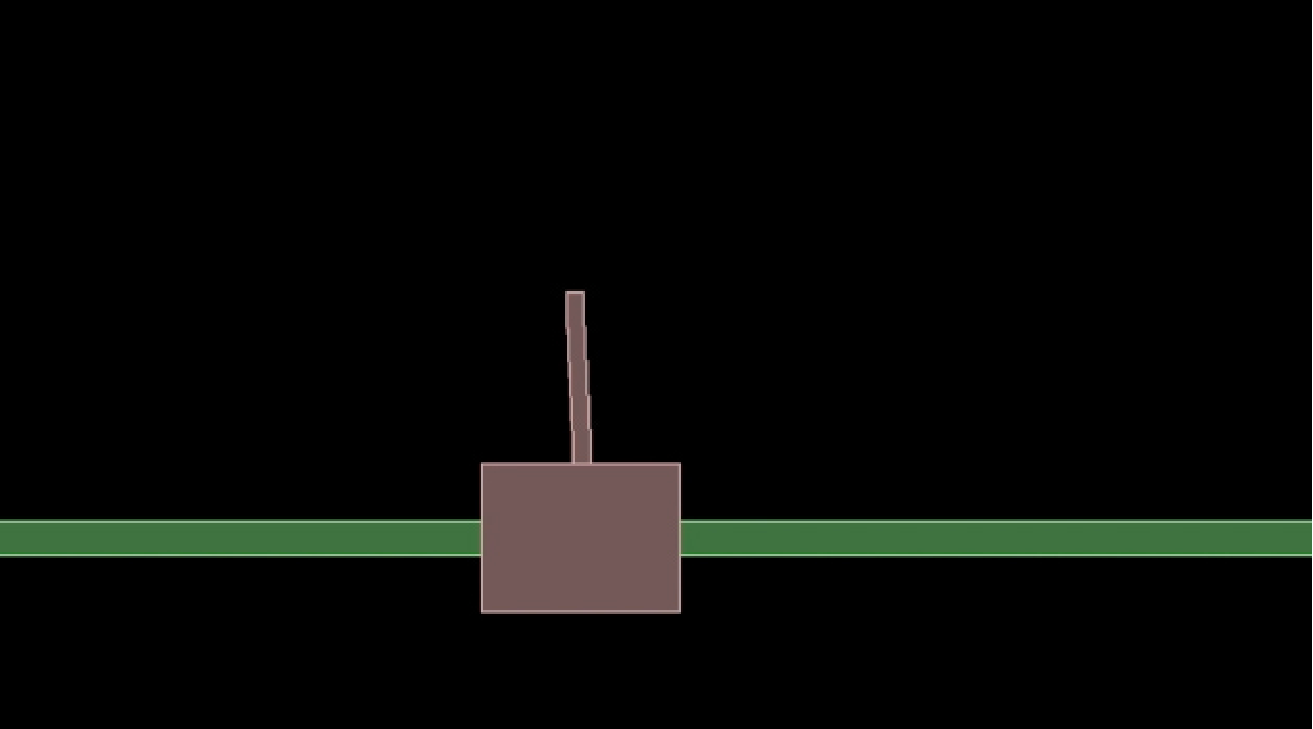
\includegraphics[width=1\textwidth]{Images/Experiments/cart.pdf}
		\vspace{-0.1in}
		\caption{Cart-Pole}
		\label{fig:cartpoletask}
	\end{minipage}
	\begin{minipage}[t]{0.32\textwidth}
		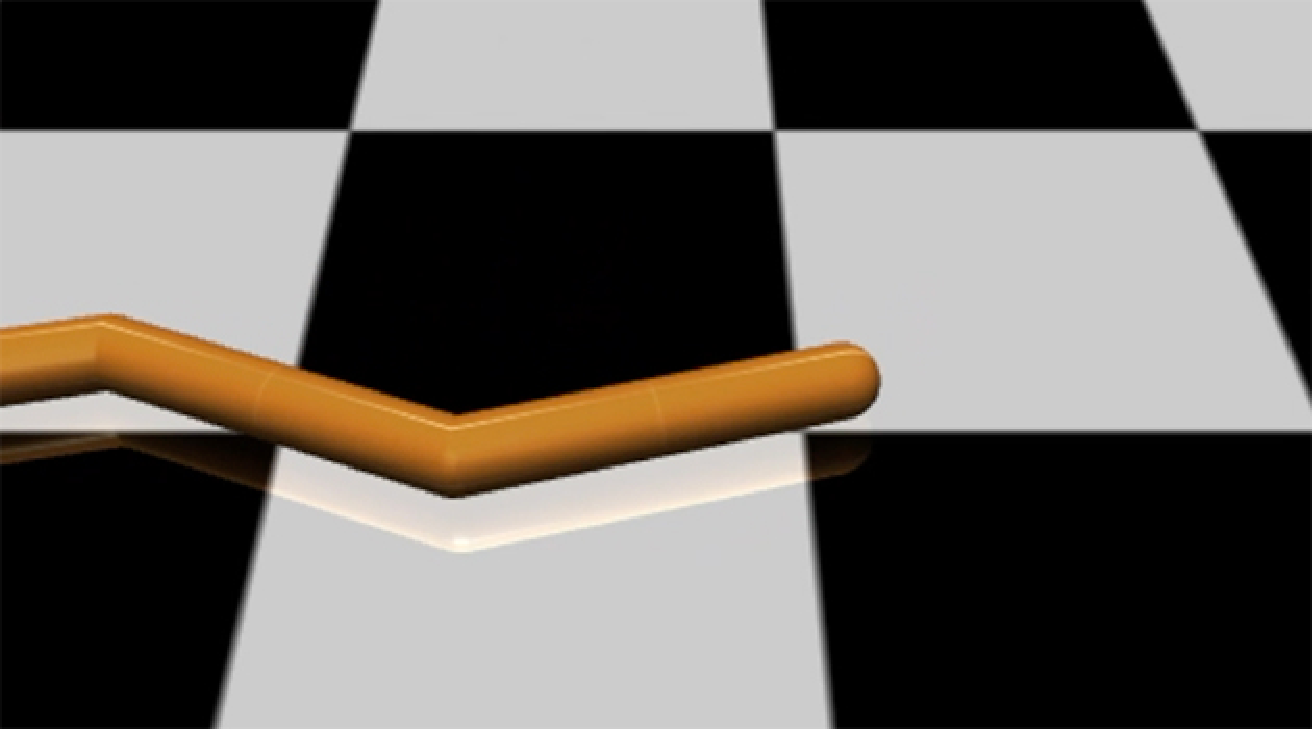
\includegraphics[width=1\textwidth]{Images/Experiments/swimmer.pdf}
		\vspace{-0.1in}
		\caption{Swimmer}
		\label{fig:swimmertask}
	\end{minipage}
	\begin{minipage}[t]{.34\textwidth}
		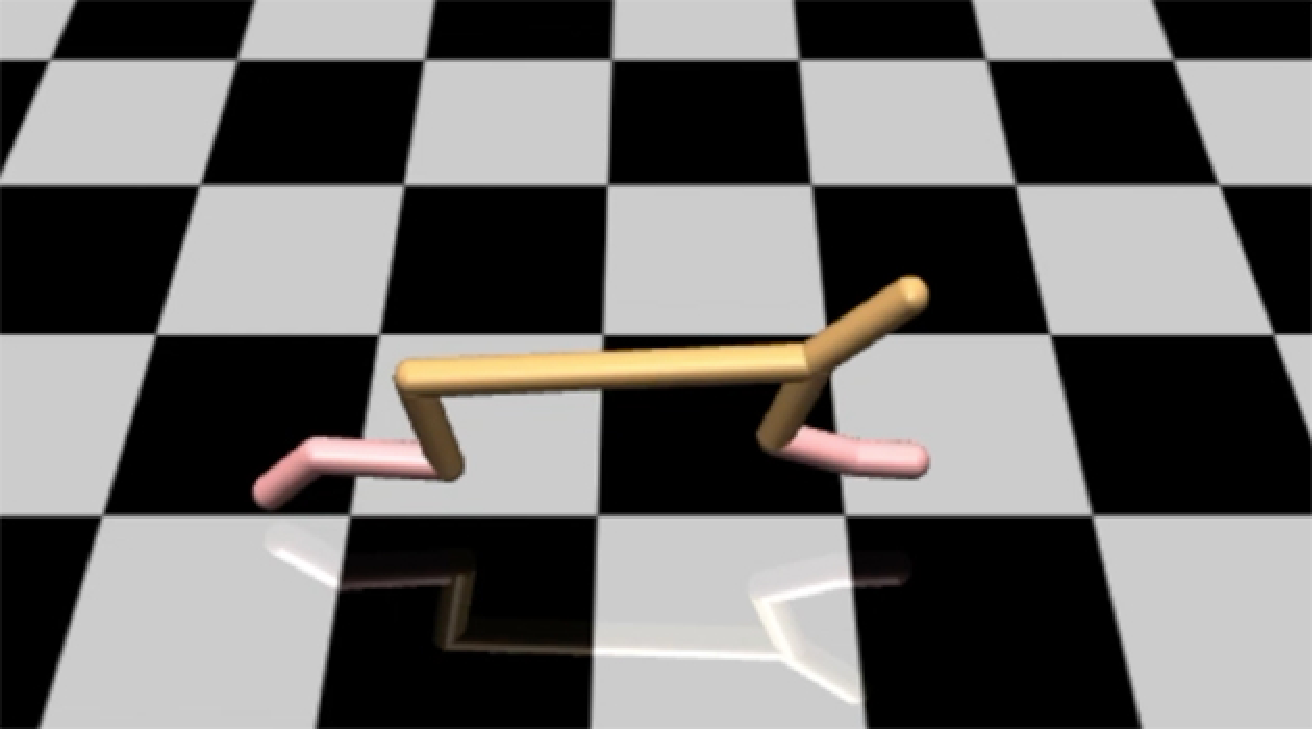
\includegraphics[height=60,width=1\textwidth]{Images/Experiments/half.pdf}
		\vspace{-0.1in}
		\caption{Half-Cheetah}
		\label{fig:halfcheetahtask}
	\end{minipage}
	\vspace{-0.15in}
\end{figure*}

All the parameters used in the experiments, including neural network architectures, are reported in the following table:

\begin{table}[H]\caption{Parameters used in the experiments. Where not specified, meta-parameters are shared among G(PO)MDP and SVRPG.}\label{table:metaparams}
	\centering
	\resizebox{\columnwidth}{1.4in}{
	\begin{tabular}{| l | c  c  c |}
		\hline	
		& Cart-Pole & Swimmer & Half Cheetah \\
		\hline
		NN hidden weights & 8 & 32x32 & 100x50x25 \\
		NN activation & tanh & tanh & tanh \\
		Adam $\alpha$ (SVRPG) & $5\cdotp10^{-2}$ & $10^{-3}$ & $10^{-3}$ \\
		Adam $\alpha$ (GPOMDP 10) & $10^{-2}$ & $10^{-3}$ & $10^{-3}$ \\ 
		Adam $\alpha$ (GPOMDP 100) & $10^{-2}$ & $10^{-2}$ & $10^{-2}$ \\ 
		Adam $\beta_1$ & 0.9 & 0.9 & 0.9 \\
		Adam $\beta_2$ & 0.99 & 0.99 & 0.99 \\ 
		Snapshot batch size $N$ (SVRPG) & 100 & 100 & 100 \\
		Mini-batch size $B$ (SVRPG) & 10 & 10 & 10 \\
		Batch size (GPOMDP) & 10 or 100 & 10 or 100 & 10 or 100\\
		Max number of sub-iterations & 50 & 20 & 20 \\
		Task horizon& 100 & 500 & 500 \\
		Baseline& No & No & Yes \\
		Discount factor $\gamma$& 0.99 & 0.995 & 0.99 \\
		Total number of trajectories& 10000 & 20000 & 50000 \\
		\hline  
	\end{tabular}
	}
\end{table}
Let us be a little bit more precise about the neural network role: given an observation it will predict mean and standard deviation of the gaussian distribution from which we will need to sample our action. Refer to \cite{duan2016benchmarking} for more details about G(PO)MDP (REINFORCE in the paper) on the Half Cheetah task.


Now we can properly anddress the main results of our work. Figure \ref{fig:cartpole} compares \acs{SVRPG} versus G(PO)MDP with batch size set to $10$ on a continuous variant of the classical Cart-pole task, which is a 2D balancing task. Despite using more trajectories on average for each parameter update, our algorithm shows faster convergence, which can be ascribed to the better quality of updates due to variance reduction. The same can be said \wrt figure \ref{fig:cartpole100}.
\begin{figure*}[h]
	\begin{minipage}[h]{1\textwidth}
		\centering
		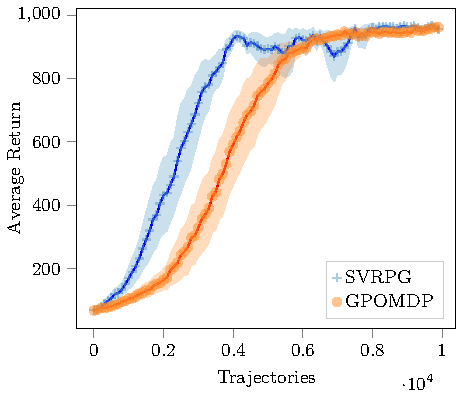
\includegraphics[width=0.65\textwidth]{Images/Experiments/cart_pole_SVRPG_vs_GPOMDP_tex.pdf}
		\vspace{-0.1in}
		\caption{On-line performance over sampled trajectories of \acs{SVRPG} vs G(PO)MDP (batch size set to 10) in the Cart-pole task, with 90\% confidence intervals.}
		\label{fig:cartpole}
	\end{minipage}
	\vspace{-0.15in}
\end{figure*}
\begin{figure*}[h]
	\begin{minipage}[h]{1\textwidth}
		\centering
		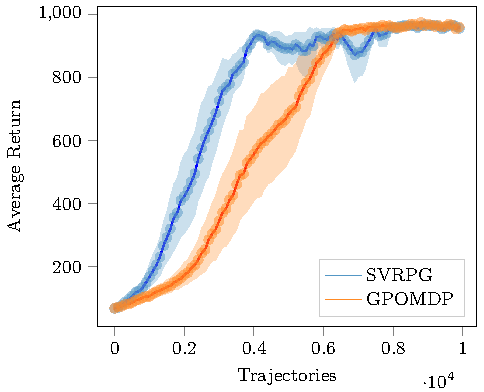
\includegraphics[width=0.65\textwidth]{Images/Experiments/cart_pole_GPOMDP_100_vs_SVRPG.pdf}
		\vspace{-0.1in}
		\caption{On-line performance over sampled trajectories of \acs{SVRPG} vs G(PO)MDP (batch size set to 100) in the Cart-pole task, with 90\% confidence intervals.}
		\label{fig:cartpole100}
	\end{minipage}
	\vspace{-0.15in}
\end{figure*}
\newpage
The Swimmer task is a 3D continuous-control locomotion task over a plane. This task is more difficult than cart-pole. In particular, the longer horizon and the more complex dynamics can have a dangerous impact on the variance of importance weights.

\begin{figure*}[h]
	\begin{minipage}[h]{1\textwidth}
		\centering
		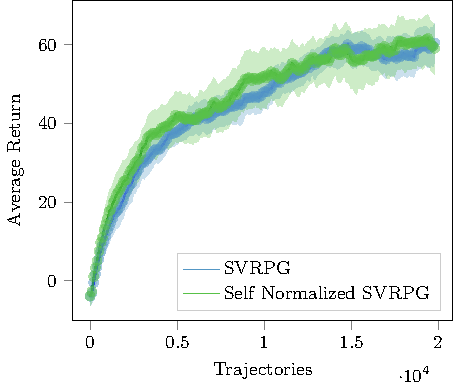
\includegraphics[width=0.65\textwidth]{Images/Experiments/swimmer_self_normalized_SVRPG_vs_SVRPG_tex.pdf}
		\vspace{-0.1in}
		\caption{On-line performance over sampled trajectories of self-Normalized \acs{SVRPG} vs unbiased \acs{SVRPG} in the Swimmer task, with 90\% confidence intervals.}
		\label{fig:swimmertwo}
	\end{minipage}
	\vspace{-0.15in}
\end{figure*}

 In this case, the self-normalization technique proposed in Section \ref{sec:prac} brings an improvement (even if not statistically significant), as shown in Figure \ref{fig:swimmertwo}.
\begin{figure*}[h]
	\begin{minipage}[h]{1\textwidth}
		\centering
		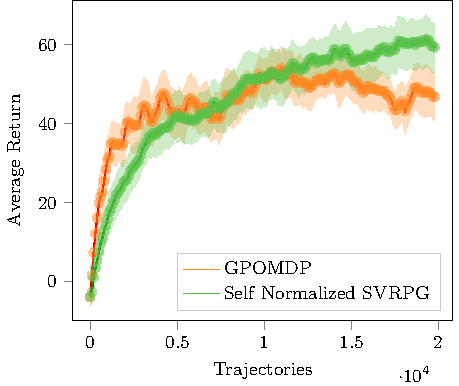
\includegraphics[width=0.65\textwidth]{Images/Experiments/swimmer_self_normalized_SVRPG_vs_GPOMDP_tex.pdf}
		\vspace{-0.1in}
		\caption{On-line performance over sampled trajectories of self-Normalized \acs{SVRPG} vs G(PO)MDP (batch size set to 10) in the Swimmer task, with 90\% confidence intervals}
		\label{fig:swimmerone}
	\end{minipage}
	\vspace{-0.15in}
\end{figure*}
\begin{figure*}[h]
	\begin{minipage}[h]{1\textwidth}
		\centering
		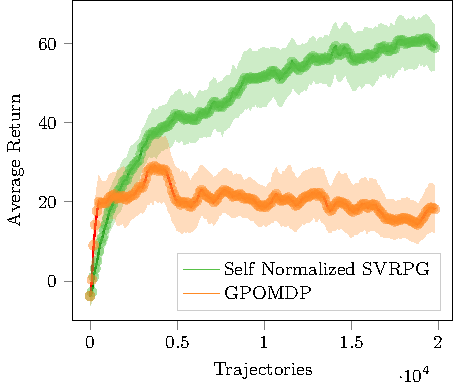
\includegraphics[width=0.65\textwidth]{Images/Experiments/swimmer_GPOMDP_100_vs_SN_SVRPG.pdf}
		\vspace{-0.1in}
		\caption{On-line performance over sampled trajectories of self-Normalized \acs{SVRPG} vs G(PO)MDP (batch size set to 100) in the Swimmer task, with 90\% confidence intervals}
		\label{fig:swimmer100}
	\end{minipage}
	\vspace{-0.15in}
\end{figure*}
% Although the confidence intervals are never disjoint, the average of the self-normalized version is always higher, which we consider enough to employ the variant in the next comparison. 
Figure \ref{fig:swimmerone} shows self-normalized \acs{SVRPG} against G(PO)MDP with batch size set to $10$. Our algorithm outperforms G(PO)MDP for almost the entire learning process. Here, toward the end of the learning process, we note that the improvement becomes statistically significant.

For what concern figure \ref{fig:swimmer100}, where we have self-normalized \acs{SVRPG} versus G(PO)MDP with batch size set to $100$, we can see that our algorithm totally outperforms G(PO)MDP and the difference in performaces is also statistically significant.

Table \ref{tab:1} compares G(PO)MDP and \acs{SVRPG} in terms of the average return computed on the whole learning process, which is a common metric for online learning since it is related to an average regret~\citep[\eg][]{duan2016benchmarking}. This metric can be visualized as the area below the curves. Note that the convergence result in Theorem \ref{theo:convergence} is precisely about the average return. We also report normalized standard deviations and 90\% $t$-confidence intervals.
In both tasks, our algorithm has higher average return and lower normalized standard deviation.
In Cart-pole, disjoint confidence intervals show that the advantage is statistically significant.

\begin{table*}[h]
	\caption{
		\label{tab:1}
		Comparison between G(PO)MDP and \acs{SVRPG} on different tasks. Average return over the whole learning process is reported, together with normalized standard deviation and 90\% confidence intervals.}
	\centering
	\begin{tabular}{@{}lccccccc@{}} 
		\toprule
		\phantom{abc} & \multicolumn{3}{c}{G(PO)MDP $10$} \\
		\cmidrule{2-4}
		\phantom{abc} & Avg Return & Norm. Std & C.I.
		\\\cmidrule{2-4}
		Cart-pole & $618.49$ & $21.09$ & $[579.82, 657.16]$\\
		Swimmer & $45.10$ & $2.37$ & $[40.13, 50.07]$\\
		Half-cheetah & $1263.59$ & $212.73$ & $[810.09, 1717.09]$\\
		\\\cmidrule{2-4}
		\phantom{abc} & \multicolumn{3}{c}{G(PO)MDP $100$} \\
		\cmidrule{2-4}
		\phantom{abc} & Avg Return & Norm. Std & C.I.
		\\\cmidrule{2-4}
		Cart-pole & $608.78$ & $28.66$ & $[556.23, 661.33]$\\
		Swimmer & $20.03$ & $2.56$ & $[15.61, 24.46]$\\
		Half-cheetah & $966.59$ & $173.14$ & $[597.49, 1335.69]$\\
		\\\cmidrule{2-4}
		\phantom{abc} & \multicolumn{3}{c}{SVRPG}
		\\\cmidrule{2-4}
		\phantom{abc} & Avg Return & Norm. Std & C.I.
		\\\cmidrule{2-4}
		Cart-pole & $736.31$ & $16.51$ & $[706.04, 766.57]$\\
		Swimmer & $46.48$ & $2.86$ & $[40.49, 52.46]$\\
		Half-Cheetah & $1397.07$ & $66.74$ & $[1254.78, 1539.36]$\\
		\bottomrule
	\end{tabular}
	\vspace{-0.05in}
\end{table*}

\subsection{Preliminary Results on Actor-Critic.}\label{subsec:actorcritic} %As mentioned, 
Another variance-reduction technique in policy gradient consists in using baselines or \textit{critics}. This tool is orthogonal to the methods described in this composition, and the theoretical results of \hyperref[chap:convergence]{Chapter 4} are general in this sense. In the experiments described so far, we compared against the so-called \textit{actor-only} G(PO)MDP, \ie without the baseline. To move towards a more general understanding of the variance issue in policy gradient, we also test \acs{SVRPG} in an \textit{actor-critic} scenario. To do so, we consider the more challenging MuJoCo~\citep{todorov2012mujoco} Half-cheetah task, a 3D locomotion task that has a larger state-action space than Swimmer. Table \ref{tab:1} also reports the comparison between \acs{SVRPG} and G(PO)MDP\footnote{\citet{duan2016benchmarking} report results on REINFORCE. However, inspection on \textit{rllab} code and documentation reveals that it is actually \ac{PGT} \citep{sutton2000policy}, which is equivalent to G(PO)MDP \citep[shown by][]{peters2008reinforcement}. Using the name REINFORCE in a general way is inaccurate, but widespread.} on Half-cheetah using the critic suggested in \cite{duan2016benchmarking} for both algorithms. More precisely, this critic is a linear state-value function estimator. 
The (time-varying) feature encoding for the linear baseline is:
\begin{align*}
\vphi(s,t)=[s, s \odot s, 0.01t, (0.01t)^2, (0.01t)^3,1],
\end{align*}
where $s\in\mathbb{R}^d$ is the state vector and $\odot$ is the element-wise product. The baseline is then:
\[
b(s_t,a_t) = \boldsymbol{\lambda}^T\vphi(s_t,t).
\]
The baseline is fitted from scratch at each policy gradient iteration, with least squares, to match state-value function $V^{\pi}(s)$.
When used with \acs{SVRPG}, the critic parameter $\boldsymbol{\lambda}$ is updated only at the snapshot. Table \ref{tab:1} shows promising results, meaning that a combination of the baseline usage and \acs{SVRG}-like variance reduction can yield an improvement that the two techniques alone are not able to achieve. For a more thorough evaluation on Half-Cheetah, together with table \ref{tab:1}, also see figure \ref{fig:hcone} and figure \ref{fig:hctwo}. In the former figure we see how our algorithm has a lot less variance and a higher mean even though the confidence intervals are not disjoint. Whereas in the latter figure we can clearly see how the self-normalization can improve the performance of our algorithm. Furthermore, for completeness, we also show in figure \ref{fig:hc100} G(PO)MPD with batch size set to $100$ against \acs{SVRPG}. Here our algorithm has a better performance accross all the learning process. More over this difference becomes statistically significant after half of the learning process itself. 
\begin{figure*}[h]
	\begin{minipage}[h]{1\textwidth}
		\centering
		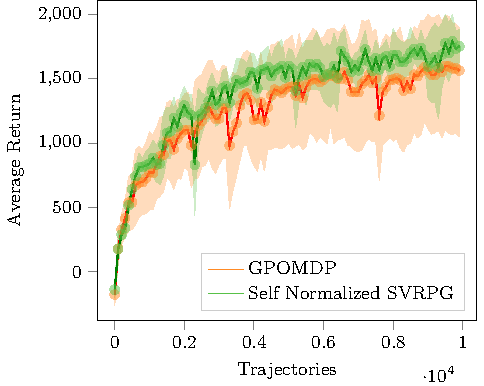
\includegraphics[width=0.65\textwidth]{Images/Experiments/half_cheetah_Self_Normalized_SVRPG_vs_GPOMDP.pdf}
		\vspace{-0.1in}
		\caption{On-line performance over sampled trajectories of self-Normalized \acs{SVRPG} vs G(PO)MDP (batch size set to 10) in the Half-Cheetah task, with 90\% confidence intervals}
		\label{fig:hcone}
	\end{minipage}
	\vspace{-0.15in}
\end{figure*}
\begin{figure*}[h]
	\begin{minipage}[h]{1\textwidth}
		\centering
		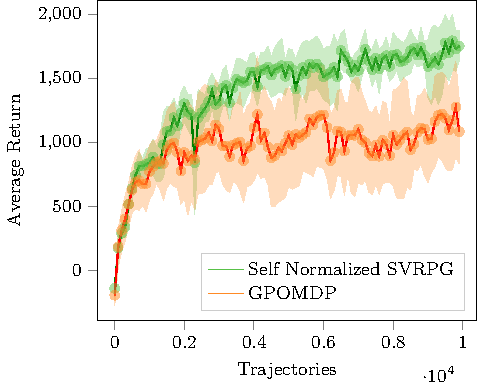
\includegraphics[width=0.65\textwidth]{Images/Experiments/half_cheetah_GPOMDP_100_vs_SN_SVRPG.pdf}
		\vspace{-0.1in}
		\caption{On-line performance over sampled trajectories of self-Normalized \acs{SVRPG} vs G(PO)MDP (batch size set to 100) in the Half-Cheetah task, with 90\% confidence intervals}
		\label{fig:hc100}
	\end{minipage}
	\vspace{-0.15in}
\end{figure*}
\begin{figure*}[t]
	\begin{minipage}[t]{1\textwidth}
		\centering
		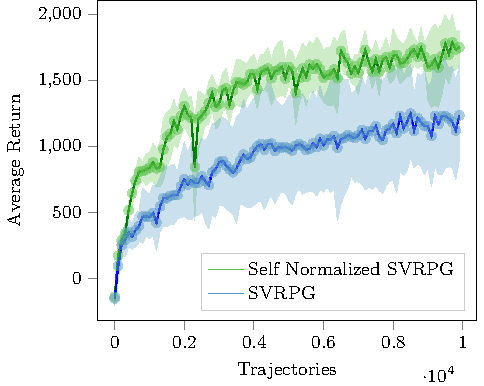
\includegraphics[width=0.65\textwidth]{Images/Experiments/half_cheetah_SVRPG_vs_SN_SVRPG.pdf}
		\vspace{-0.1in}
		\caption{On-line performance over sampled trajectories of self-Normalized \acs{SVRPG} vs unbiased \acs{SVRPG} in the Half-Cheetah task, with 90\% confidence intervals.}
		\label{fig:hctwo}
	\end{minipage}
	\vspace{-0.15in}
\end{figure*}
\newpage
\subsection{Exploratory Results on Other Gradient Estimators}\label{subsec:oge}
Another preliminary attempt was made using different gradient estimators in our algorithm. Therefore equation \eqref{E:svrpg.estimate.batch} has been rearranged in order to get new gradient estimators. Here we report the obtained expressions:

\begin{align}\label{E:svrpg.b.version}
	\blacktriangledown J(\vtheta_{t}) &:= v_t= \wh{\nabla}_N J(\wt{\vtheta})\\ \notag
	& \quad{} + 
		\frac{1}{B} \sum_{i=0}^{B-1} \left[
		\omega(\tau_i|\wt{\vtheta}, \vtheta_t)g(\tau_i|\wt{\vtheta}) - g(\tau_i|\wt{\vtheta})
		\right]
\end{align}
where the sampling distribution is $\pi_{\wt{\vtheta}}$ for the mini-batch terms.
\begin{align}\label{E:svrpg.c.version}
	\blacktriangledown J(\vtheta_{t}) &:= v_t= \frac{1}{N}\sum_{i=1}^{N} \omega(\tau_i|\wt{\vtheta}, \vtheta_t)g(\tau_i|\wt{\vtheta})\\\notag & \quad{} + 
		\frac{1}{B} \sum_{i=0}^{B-1} \left[
		g(\tau_i|\vtheta_t) - g(\tau_i|\wt{\vtheta})
		\right]
\end{align}
where the sampling distribution is $\pi_{\vtheta_t}$ for the mini-batch terms.\newline
Since equation \ref{E:svrpg.b.version} has $\pi_{\wt{\vtheta}}$ as sampling distribution in the sub-iterations, we can avoid sampling from the environment randomly picking $B$ trajectories from those ones obtained for the snapshot, hence saving a lot of data. Note that in this way we have introduced a bias which, however, is legitimated by the huge data saving. Furthermore, being this version off policy, we have the importance weights exactly on the term we want an estimate of. This latter feature could be dangerous in tasks with a lot of stochasticity, because the variance on the importance weights could dramatically ruin the quantity we want to estimate. Whereas equation \ref{E:svrpg.c.version} has the importance weights binded to the term with $N$ trajectories, which better shrinks the variance contribution of the weights themselves \wrt when they were binded to the term with $B$ trajectories. Notice that the two terms that cancel in expected value do not mean anything when considered alone. From now on we refer to our algorithm based on equation \ref{E:svrpg.b.version} as \acs{SVRPG} B version if it does not reuse the trajectories of the snapshot and \acs{SVRPG} BR if it does, whereas we refer to our algorithm based on equation \ref{E:svrpg.c.version} as \acs{SVRPG} C version.\newline
The results coming from the usage of these new estimators within our algorithm are not satisfying except for the equation \ref{E:svrpg.b.version} version in cart-pole (see \hyperref[chap:appendix]{Appendix A} for the experimental results). These outcomes are due to the fact that the work performed in these directions is currently at an early stage and would need a more thoughtful approach in order to have a chance to make them properly work in practice.

\vspace{-0.05in}
	
	% ************************************************************
	% Backmatter
	%*************************************************************
	\cleardoublepage%********************************************************************
% Bibliography
%*******************************************************
% work-around to have small caps also here in the headline
\manualmark
\markboth{\spacedlowsmallcaps{\bibname}}{\spacedlowsmallcaps{\bibname}}
%\phantomsection 
\refstepcounter{dummy} 
% to have the bib a bit from the rest in the toc
\addtocontents{toc}{\protect\vspace{\beforebibskip}}
\addcontentsline{toc}{chapter}{\tocEntry{\bibname}}
\label{app:bibliography} 
\printbibliography
	\appendix
	% \cleardoublepage\part{Appendix}
	%********************************************************************
% Appendix
%*******************************************************
% If problems with the headers: get headings in appendix etc. right
\markboth{\spacedlowsmallcaps{Appendix}}{\spacedlowsmallcaps{Appendix}}
%************************************************
\chapter{Appendix example: code listings}

\begin{flushright}{\slshape    
    We have seen that computer programming is an art, \\ 
    because it applies accumulated knowledge to the world, \\ 
    because it requires skill and ingenuity, and especially \\
    because it produces objects of beauty.} \\ \medskip
    --- \citeauthor{knuth:1974}, \citetitle{knuth:1974},
\citeyear{knuth:1974} 
\end{flushright}

\section{The \texttt{listings} package to include source code}
Source code is usually not part of the text of a thesis, but if it is an original contribution it makes sense to le the code speak by itself instead of describing it. The package \verb!listings! provide the proper layout tools. Refer to its manual if you need to use it, an example is given in listing \ref{lst:probCounter}.

\lstinputlisting[
	firstline=1,
	lastline=47,
	float=tb,
	language=C++,
	tabsize=2,
	numbers=left,
	numberstyle=\tiny,
	stepnumber=2,
	numbersep=5pt,
	caption={Code snippet with the recursive function to evaluate the pdf of the sum $Z_N$ of $N$ random variables equal to $X$.}, 
	captionpos=t,
	label=lst:probCounter
	]{CodeFiles/probabilityCounter.cpp}

\end{document}
% ****************************************************************